% Opciones empleadas:
%
%	a4paper -> indica el tama�o del papel, en este caso A4.
%	11pt -> tama�o de la fuente 11 puntos.
%	oneside -> s�lo escribimos en una cara del folio.
% 
% Otras opciones interesantes:
%
%	twoside -> escribimos a doble cara.
%	openbib -> para que las referencias bibliogr�ficas tengan un salto de l�nea entre cada campo de la referencia.
%
\documentclass[a4paper,11pt,oneside]{book}

% codificaci�n latin1 y s�mbolos del idioma espa�ol (�, acentos, ...)
\usepackage[spanish]{babel}
\usepackage[latin1]{inputenc}
\usepackage{float}

% puede que queramos usar el s�mbolo del euro.
\usepackage{eurosym}

% El paquete fancybox nos permite crear cajas de diferentes estilos con facilidad.
% http://www.ctan.org/get/macros/latex/contrib/fancybox/fancybox.pdf
% http://www.mackichan.com/index.html?techtalk/487.htm~mainFrame
\usepackage{fancybox}
\usepackage{multicol}
\usepackage{amsmath}

% Para incluir subfiguras.
\usepackage{subcaption}

% Para incluir gr�ficos en JPG => compilar con pdflatex.
% \usepackage[pdftex]{graphicx}

% Para incluir gr�ficos EPS => compilar con latex.
\usepackage[pdftex]{graphicx}
\usepackage[outdir=./]{epstopdf}

% Para escribir en color...
%
% ... cuando compilamos con el comando ``latex''
\usepackage[pdftex,usenames,dvipsnames]{color}
% ... uando compilamos con el comando ``pdflatex''
% \usepackage[pdftex,usenames,dvipsnames]{color}

% Espaciado y ajuste de m�rgenes
\usepackage{setspace}
\onehalfspacing
% \doublespacing
\setlength{\textwidth}{15cm}
\setlength{\textheight}{22cm}
\setlength{\oddsidemargin}{1cm}
\setlength{\evensidemargin}{1cm}

\usepackage{listings}
%Landscape figures.
\usepackage{lscape}
\usepackage{wrapfig}

% Paquete fancyhdr -> Para modificar la cabecera y pie de p�ginas.
% http://tug.ctan.org/tex-archive/macros/latex/contrib/fancyhdr/
\usepackage{fancyhdr}
\pagestyle{fancy}
\fancyhf{}
\fancyhf[HR]{\thepage}
\fancyhf[HL]{\nouppercase\rightmark}

% Package booktabs -> Para mejorar el aspecto de las tablas o cuadros.
% http://www.ctan.org/tex-archive/macros/latex/contrib/booktabs/
\usepackage{booktabs}

% Package rotating -> Para poder girar las tablas y dibujarlas a lo largo
% del folio en vez de a lo ancho.
\usepackage{rotating}

% Packages multicol y multirow, para manejar tablas de filas y columnas m�ltiples.
\usepackage{multicol}
\usepackage{multirow}

% Personalizamos la separaci�n entre p�rrafos...
\parskip=6pt

% Personalizamos el identado en la primera l�nea del nuevo p�rrafo...
\parindent=10pt

% Establecemos el n�mero m�ximo de niveles de profundidad en las secciones.
\setcounter{secnumdepth}{3}

% T�tulo
\title{Visualizaci�n avanzada de nubes de puntos con OpenGL}
% Autor
\author{David Ant�nez Gonz�lez}
% Fecha
\date{\today}


\begin{document}

	% \maketitle sirve para generar autom�tica una portada predefinida, pero para un proyecto fin de carrera
	%	de FIC no sirvir�a porque no cumple las normas de presentaci�n. Podemos hacer dos cosas:
	% 1. Usarla e ignorar las normas (y asumir las consecuencias que pueda tener)
	% 2. Hacernos una portada en LaTeX que cumpla las normas (menos arriesgado)
	%
        %
% Portada.
%

% Nota: Ser�a m�s c�modo emplear el comando \maketitle que genera una portada de forma autom�tica, pero 
% no incluye toda la informaci�n que es necesario incluir en la memoria de un proyecto de fin de carrera
% de la Facultad de Inform�tica de A Coru�a.
%

\begin{titlepage}

	\begin{center}

		% Logotipo de la universidad.
		
\includegraphics[width=6cm]{../figures/anagrama.png}
		\vspace{2cm}

		% Nombre de la facultad, de la universidad y del departamento en que se realiza el PFC.
		{\Large{\textbf{Facultad de Inform�tica de la Universidad de A Coru�a}}}
		\\
		{\it \large{\textbf{Electr�nica y Sistemas}}}
		\vspace{1cm}

		% Indicamos el nombre de la titulaci�n oficial que hemos cursado con tanto esfuerzo.
		{\large PROYECTO DE FIN DE CARRERA\\INGENIERIA T�CNICA EN INFORM�TICA DE SISTEMAS}
		\vspace{1cm}

		% T�tulo
		\textbf{\Large Visualizaci�n avanzada de nubes de puntos con OpenGL}
		\vspace{7cm}
	\end{center}

	\begin{flushright}
		\begin{tabular}{ll}
			% Nombre del alumno.
			\large{\textbf{Alumno:}}	&
			\large{Ant�nez Gonz�lez, David} \\

			% Nombre del director/tutor del proyecto.
			\large{\textbf{Director:}}	&
			\large{�lvarez Mures, Luis Omar} \\

			% Nombre del director/tutor del proyecto.
			\large{\textbf{Tutor y Director:}}	&
			\large{Padr�n Gonz�lez, Emilio Jos�} \\
			
			% Fecha.
			\large{\textbf{Fecha:}}	&
			\large{\today} \\
		\end{tabular}
	\end{flushright}

\end{titlepage}


	% FRONTMATTER: TOC, LOF, LOT y descripci�n/organizaci�n de la memoria.
        \frontmatter

	% Los proyectos de fin de carrera de FIC han de ir acompa�ados de una serie de documentos adicionales, algunos
	% 	de ellos obligatorios (certificado, resumen, lista de palabras clave) y otros opcionales (dedicatoria
	%	y agradecimientos).
	%
        \thispagestyle{empty}     % No number page, headings...
        %
% Certificado
%

\begin{center}
	\begin{minipage}[t][6cm][l]{.8\textwidth}
		\begin{center}
			% Nombre del director del proyecto
			D. {\sc Nombre Del Director del Proyecto}

			% A los profesores les gusta que se indique su grado o posici�n en la estructura de la universidad :-P
			Profesor de Escuela o Facultad Universitaria

			% Departamento al que pertenece el director y en el que se realiza el proyecto.
			Departamento de lo que sea

			Universidad de A Coru�a
		\end{center}
	\end{minipage}
\end{center}

% El director certifica que el proyecto obra de su proyectando constituye su Proyecto de Fin de Carrera en la titulaci�n indicada.
CERTIFICA:
Que la memoria titulada {\it ``Lorem ipsum dolor sit amet, consectetuer adipiscing elit vestibulum a pede sit amet augue pellentesque''} ha sido realizada por {\sc Mauro Silvosa Rivera} bajo mi direcci�n y constituye su Proyecto de Fin de Carrera de Nombre de la Titulaci�n Que Corresponda.

\vspace{5cm}

En A Coru�a, a \today

% Espacio para que pueda firmar el certificado que debe acompa�ar al proyecto.
\vspace{3cm}

\begin{center}
	\begin{minipage}[t][4cm][l]{.5\textwidth}
	% Nombre del director del proyecto
	D. {\sc Nombre Del Director del Proyecto}
	\\
	Director del proyecto
	\end{minipage}
\end{center}

        \thispagestyle{empty}     % No number page, headings...

        %
% Resumen del proyecto de fin de carrera
%

\section*{Resumen:}

El render de nubes de puntos adquiri� un renovado inter�s en los �ltimos a�os con la popularizaci�n y proliferaci�n de nuevos sistemas de adquisici�n de datos de de datos de alto/medio coste, habitualmente basados en un esc�ner l�ser basado en la tecnolog�a conocida como LiDAR, o de bajo coste, basados en fotogametr�a o c�maras infrarrojas.

Estos dispositivos obtienen una nube de puntos 3D (posici�n geom�trica), con informaci�n adicional arbitraria asociada, normalmente el color como m�nimo, aunque tambi�n son habituales otros datos como normales, temperatura, etc. Por las propias caracter�sticas que tiene el punto como primitiva gr�fica, respecto por ejemplo de los tradicionales pol�gonos habitualmente empleados en inform�tica gr�fica (no tienen �rea, no tienen orientaci�n, no est�n conectados, etc.), el render o visualizaci�n de nubes de puntos presenta una serie de retos si queremos obtener una visualizaci�n realista y de calidad. 

Este proyecto se centra en la visualizaci�n avanzada de nubes de puntos, aplicando algunas de las mas novedosas t�cnicas de render y haciendo uso de las caracter�sticas avanzadas de la API gr�fica multiplataforma OpenGL, lo que nos permite explotar el hardware de las tarjetas gr�ficas modernas. El resultado del proyecto ser� la implementaci�n de una herramienta multiplataforma para la visualizaci�n avanzada de nubes de puntos 3D.

        \thispagestyle{empty}     % No number page, headings...

        %
% Palabras clave
%

\section*{Lista de palabras clave:}

Lorem ipsum, dolor sit amet, consectetuer, adipiscing elit, vestibulum a pede, sit amet augue, pellentesque ,vehicula, donec pretium.



        \thispagestyle{empty}     % No number page, headings...

        %
% Dedicatoria
%
\section*{}

\begin{flushright}
	{\it Knight Rider, a shadowy flight into the dangerous world of a man who does not exist. Michael Knight, a young loner on a crusade to champion the cause of the innocent, the helpless in a world of criminals who operate above the law.}
\end{flushright}

        \thispagestyle{empty}     % No number page, headings...

        %
% Agradecimientos
%

\section*{Agradecimientos}

A �ngela la persona a la que le dedico y dedicar� siempre.

A mi familia que me acompa�� y pag� mis matr�culas todos estos a�os y con las que se podr�an haber comprado un piso en Marbella pero prefirieron que su hijo estudiara.

A Emilio y Omar, a los que considero amigos y que sin su ayuda quiz�s este instante de escribir dedicatorias no hubiese existido jam�s. Gracias :)


        \thispagestyle{empty}     % No number page, headings...

        \tableofcontents
        \listoffigures
        \listoftables

        %
% Frontmatter - Introducci�n. Los miembros del tribunal que juzgan los PFC's tienen muchas m�s memorias que leer, por lo que
%	agradecer�n cualquier detalle que permita facilitarles la vida. En este sentido, realizar una peque�a introducci�n,
%	comentar la organizaci�n y estructura de la memoria y resumir brevemente cada cap�tulo puede ser una buena pr�ctica
%	que permita al lector centrarse f�cilmente en la parte que m�s le interesa.
%

\chapter[Introducci�n]{
	Introducci�n
}

One for all and all for one, Muskehounds are always ready. One for all and all for one, helping everybody. One for all and all for one, it's a pretty story. Sharing everything with fun, that's the way to be. One for all and all for one, Muskehounds are always ready. One for all and all for one, helping everybody. One for all and all for one, can sound pretty corny. If you've got a problem chum, think how it could be.

Hong Kong Phooey, number one super guy. Hong Kong Phooey, quicker than the human eye. He's got style, a groovy style, and a car that just won't stop. When the going gets tough, he's really rough, with a Hong Kong Phooey chop (Hi-Ya!). Hong Kong Phooey, number one super guy. Hong Kong Phooey, quicker than the human eye. Hong Kong Phooey, he's fan-riffic!

Ten years ago a crack commando unit was sent to prison by a military court for a crime they didn't commit. These men promptly escaped from a maximum security stockade to the Los Angeles underground. Today, still wanted by the government, they survive as soldiers of fortune. If you have a problem and no one else can help, and if you can find them, maybe you can hire the A-team.

This is my boss, Jonathan Hart, a self-made millionaire, he's quite a guy. This is Mrs H., she's gorgeous, she's one lady who knows how to take care of herself. By the way, my name is Max. I take care of both of them, which ain't easy, 'cause when they met it was MURDER!

Top Cat! The most effectual Top Cat! Who's intellectual close friends get to call him T.C., providing it's with dignity. Top Cat! The indisputable leader of the gang. He's the boss, he's a pip, he's the championship. He's the most tip top, Top Cat.


%
% SECCION
%
\subsection*{Contexto y Objetivos}

Los objetivos concretos que cubre la elaboraci�n de este proyecto fin de carrera son:
\begin{enumerate}
	\item Aprendizaje de la API gr�fica OpenGL, que permite un render interactivo multiplataforma.
	\item Visualizaci�n b�sica: Desarrollo de un visualizador multiplataforma de nubes de puntos 3D. Se har� una primera versi�n b�sica que ir� evolucionando durante todo el proyecto, incorporando las distintas t�cnicas que se vayan estudiando e implementando.
	\item Implementaci�n de t�cnicas avanzadas de visualizaci�n de nubes de puntos
	 \begin{enumerate}
	 	\item Basadas en rasterizaci�n: discos orientados, correci�n de perspectiva
		 \item Basadas en blending
	 \end{enumerate}
	\item Propuesta de un algoritmo novedoso para la visualizaci�n de puntos con blending en un �nico pase.
	\item Integraci�n del visualizador con la libter�a PCL, especializada en la gesti�n de nubes de puntos. Esto nos permitir� acceder a un importante abanico de m�todos y estructuras para el trabajo eficiente con grandes conjuntos de datos.
\end{enumerate}


%
% SECCION
%
\subsection*{Estructura de la memoria}

La memoria est� constituida por un total de 6 cap�tulos, en los que ser ir�n desarrollando diferentes git
In a dolor sed odio eleifend varius. Nam ullamcorper. Curabitur ut erat vulputate nisi molestie tempus. Sed aliquam rutrum odio. In mollis. Fusce consectetuer lorem nec diam. Sed mollis lacinia purus. Curabitur feugiat hendrerit neque. Quisque auctor laoreet diam. Curabitur sit amet nisi. Fusce velit massa, dignissim quis, bibendum eget, vehicula mattis, leo. Morbi auctor leo sit amet nibh. Lorem ipsum dolor sit amet, consectetuer adipiscing elit. Nullam enim. Pellentesque hendrerit, augue non vulputate semper, sem lorem pharetra nibh, sit amet egestas massa diam ac augue. In dui nulla, egestas nec, pulvinar suscipit, tincidunt ornare, nisi. Duis tristique tortor quis magna. Vestibulum faucibus lorem nec neque. Sed nec nibh. Nunc condimentum. Maecenas neque. Nullam pretium est non risus. Etiam gravida. Maecenas nisl. Fusce pharetra odio in tortor. Integer orci turpis, interdum eget, vulputate sed, tristique a, metus. Duis vitae dui quis lectus pretium aliquam. Praesent quam.

Aliquam sed orci. Cras adipiscing nisl quis pede. Ut rhoncus. Donec viverra laoreet purus. Phasellus nulla. Vivamus eget eros. In mollis aliquam orci. Proin ullamcorper. Nullam sollicitudin vestibulum lorem. Nunc malesuada sagittis augue. Donec tellus velit, dapibus a, aliquam ac, tincidunt id, lectus. 


\paragraph*{Cap�tulo 1.}
Phasellus tempor velit nec velit. Proin vitae dui a sapien commodo blandit. Etiam aliquam, sapien vitae fringilla venenatis, lectus sem accumsan orci, eget blandit orci odio et magna. Quisque malesuada, eros vel tempus eleifend, velit enim porttitor sem, eget consequat nulla neque et sapien. Morbi leo. Sed vestibulum lacus. Fusce ut lacus. Phasellus pellentesque pede eu eros. Duis turpis felis, eleifend ut, semper ac, porta nec, sem. Praesent odio. Sed laoreet mollis purus. Praesent vestibulum, velit ut mollis aliquam, quam lectus varius urna, sed ultricies erat nisl ac tortor. Vivamus tempor mauris sit amet nulla. Integer venenatis. Integer sagittis euismod ante. Suspendisse at elit. Duis eget purus nec pede adipiscing auctor. Proin ac est.

\paragraph*{Cap�tulo 2.}
Proin condimentum. Maecenas sodales. In ornare nunc a leo. Nam sit amet ligula. Nunc quis urna ac metus imperdiet lobortis. Sed quis ligula. Maecenas blandit pede. Donec lacinia rutrum ligula. Vivamus in metus vel elit pharetra molestie.

\paragraph*{Cap�tulo 3.}
Nullam ante lorem, placerat et, egestas nec, pellentesque non, sapien. Donec semper, felis id posuere faucibus, nibh ipsum tincidunt quam, et varius ipsum odio ac neque. In tincidunt dignissim diam. Sed lacus lorem, ornare ut, eleifend vel, pellentesque tempus, augue. Duis eu magna. Mauris libero ante, porttitor vel, lobortis a, mollis ac, sem. Nunc at lectus. Integer ac libero a nisl dignissim mollis. Donec velit neque, vestibulum eget, pulvinar vel, malesuada ut, nisi. Praesent congue tempus quam. Cum sociis natoque penatibus et magnis dis parturient montes, nascetur ridiculus mus.

\paragraph*{Cap�tulo 4.}
Mauris ut odio. Nulla accumsan. Morbi condimentum fermentum purus. Pellentesque habitant morbi tristique senectus et netus et malesuada fames ac turpis egestas. Nunc dignissim, neque eget convallis pretium, diam tortor fringilla lacus, a laoreet nisl metus eu magna. Cras ut lectus. Etiam accumsan feugiat elit.

\paragraph*{Cap�tulo ...}
Donec a pede. Proin dolor. Ut nunc ligula, tempor id, ornare sit amet, aliquam et, nibh. In mollis iaculis pede. Vivamus gravida orci eu nisl. Sed nibh sem, consequat at, iaculis non, placerat in, ligula. Praesent id nisi. Nunc pellentesque justo non libero. Sed quis est sit amet purus lobortis blandit. Sed arcu justo, rhoncus condimentum, ullamcorper iaculis, viverra et, nisl.

\paragraph*{Cap�tulo N.}
Fusce luctus gravida leo. Nullam dignissim arcu ac risus hendrerit rhoncus. Aliquam erat volutpat. Ut mollis, mauris non aliquam luctus, nulla sem aliquam tellus, in consequat augue odio in urna.







	% MAINMATTER: El contenido, cap�tulo a cap�tulo, de la memoria del PFC.
        \mainmatter

	%
% PLANIFICACI�N Y METODOLOG�A
%
\chapter{
	Planificaci�n y metodolog�a
	\label{nombre_referencia_al_capitulo}
}

Este cap�tulo explica el m�todo escogido para el desarrollo de este proyecto. Ya que fundamentalmente tiene una base de car�cter investigativa, se pens� que encajar�a perfectamente un sistema �gil como el que a continuaci�n se comentar� para el desarrollo del proyecto. Seguidamente de la exposici�n de un diagrama de \textit{Gantt} con los plazos e hitos que se siguieron en este caso concreto.


\section{Desarrollo �gil de software}

El desarrollo �gil de software refiere a m�todos de ingenier�a del software basados en el desarrollo iterativo e incremental, donde los requisitos y soluciones evolucionan mediante la colaboraci�n de grupos auto organizados y multidisciplinarios. Existen muchos m�todos de desarrollo �gil; la mayor�a minimiza riesgos desarrollando software en lapsos cortos. El software desarrollado en una unidad de tiempo es llamado una iteraci�n, la cual debe durar de una a cuatro semanas. Cada iteraci�n del ciclo de vida incluye: planificaci�n, an�lisis de requisitos, dise�o, codificaci�n, revisi�n y documentaci�n. Una iteraci�n no debe agregar demasiada funcionalidad para justificar el lanzamiento del producto al mercado, sino que la meta es tener una �demo� (sin errores) al final de cada iteraci�n. Al final de cada iteraci�n el equipo vuelve a evaluar las prioridades del proyecto.

Los m�todos �giles enfatizan las comunicaciones cara a cara en vez de la documentaci�n. La mayor�a de los equipos �giles est�n localizados en una simple oficina abierta, a veces llamadas "plataformas de lanzamiento" (bullpen en ingl�s). La oficina debe incluir revisores, escritores de documentaci�n y ayuda, dise�adores de iteraci�n y directores de proyecto. Los m�todos �giles tambi�n enfatizan que el software funcional es la primera medida del progreso. Combinado con la preferencia por las comunicaciones cara a cara, generalmente los m�todos �giles son criticados y tratados como "indisciplinados" por la falta de documentaci�n t�cnica.

Los m�todos de desarrollo �giles e iterativos pueden ser vistos como un retroceso a las pr�cticas observadas en los primeros a�os del desarrollo de software (aunque en ese tiempo no hab�a metodolog�as formales). Inicialmente, los m�todos �giles fueron llamados m�todos de "peso liviano".

\subsection[Agile Manifesto]{Agile Manifesto}
En el a�o 2001, miembros prominentes de la comunidad se reunieron en Snowbird, Utah, para discutir m�todos de desarrollo ligero, publicando lo que denominaron \textit{Manifesto for Agile Software Development} con motivo de sentar las bases de lo que ahora se conoce como Desarrollo �gil de software.

Siendo sus ideas principales:
\begin{itemize}
	\item \textbf{Individuos e interacciones} auto-organizaci�n y la motivaci�n son importantes. Otros valores promovidos son la co-ubicaci�n y la programaci�n en parejas.
	\item \textbf{Software funcionando} priorizando el tener \textit{demos} funcionales frente a documentaci�n. 
	\item \textbf{Colaboraci�n con el cliente} los requerimientos t�cnicos muchas veces no pueden ser definidos al principio del ciclo de desarrollo, por lo que la continua participaci�n con el cliente es muy importante
	\item \textbf{Respuesta ante el cambio} centr�ndose en respuestas r�pidas a los cambios y el desarrollo continuo.
\end{itemize}

\subsection[Principios �giles]{Principios �giles}

Este manifesto est� basado en los siguientes 12 principios:

\begin{itemize}
	\item Nuestra mayor prioridad es satisfacer al cliente
	mediante la entrega temprana y continua de software
	con valor.
	
	\item Aceptamos que los requisitos cambien, incluso en etapas 
	tard�as del desarrollo. Los procesos �giles aprovechan
	el cambio para proporcionar ventaja competitiva al 
	cliente.
	
	\item Entregamos software funcional frecuentemente, entre dos
	semanas y dos meses, con preferencia al periodo de 
	tiempo m�s corto posible.
	
	\item Los responsables de negocio y los desarrolladores
	trabajamos juntos de forma cotidiana durante todo
	el proyecto.
	
	\item Los proyectos se desarrollan en torno a individuos 
	motivados. Hay que darles el entorno y el apoyo que 
	necesitan, y confiarles la ejecuci�n del trabajo. 
	
	\item El m�todo m�s eficiente y efectivo de comunicar 
	informaci�n al equipo de desarrollo y entre sus 
	miembros es la conversaci�n cara a cara.
	
	\item El software funcionando es la medida principal de 
	progreso.
	
	\item Los procesos �giles promueven el desarrollo 
	sostenible. Los promotores, desarrolladores y usuarios
	debemos ser capaces de mantener un ritmo constante 
	de forma indefinida.
	
	\item La atenci�n continua a la excelencia t�cnica y al 
	buen dise�o mejora la Agilidad.
	
	\item La simplicidad, o el arte de maximizar la cantidad de
	trabajo no realizado, es esencial.
	
	\item Las mejores arquitecturas, requisitos y dise�os
	emergen de equipos auto-organizados.
	
	\item A intervalos regulares el equipo reflexiona sobre
	c�mo ser m�s efectivo para a continuaci�n ajustar y
	perfeccionar su comportamiento en consecuencia.
\end{itemize}

\subsection[Aplicaci�n]{Aplicaci�n}

En gran parte del proyecto, fueron aplicadas premisas e ideas propuestas en este \textit{Agile Manifesto}. Se hicieron reuniones semanales en las que se discut�an las siguientes tareas a llevar a cabo, dividiendo objetivos principales en tareas simples que no supusiesen m�s de 2 semanas de desarrollo. El trabajo en cada iteraci�n era constante, centr�ndose siempre en completar la tarea y no asumiendo cambios si no eran profundamente necesario.

El dise�o incremental fu� presente, puesto que en cada momento el dise�o era revisado para adaptarlo a los nuevos requerimientos.

Las revisiones con mis dos directores fueron siempre cara a cara mientras fue posible. En cada reuni�n se comentaba que objetivos hab�an sido cumplidos desde la �ltima vez, y que objetivos se intentar�an abordar en la siguiente iteraci�n. Cuando estas reuniones no eran posibles, sistemas como el correo electr�nico o plataformas de \textit{chat} como \textit{Hangouts} o \textit{Telegram} fueron utilizados.

Para mantener el c�digo accesible en todo el momento, desde el comienzo del desarrollo se utilizaron sistemas de control de versiones como \textit{Git}. Que es un sistema libre de administraci�n de c�digo fuente y distribuci�n. De modo que adem�s de servir como un sistema de \textit{backup} era f�cil llevar el seguimiento del desarrollo, facilitando la creaci�n de nuevas ramas paralelas a la versi�n estable, con motivo de prueba para nuevos algoritmos.

A pesar de que el evidente componente de investigaci�n que tiene este
proyecto, en el que se van a emplear t�cnicas que son ahora mismo
estado del arte en computaci�n gr�fica, imposibilita en gran medida
una adecuada estimaci�n de tiempo por cada iteraci�n, el diagrama de
\textit{Gantt} de las {\figurename}s~\ref{figure_gantt_part1} y
\ref{figure_gantt_part2} viene a resumir los tiempos que llev� cada
iteraci�n. La tabla del \tablename~\ref{tab:tareas} muestra las
principales tareas llevadas a cabo en esas interaciones.

\begin{table}
\centering
\begin{tabular}{l c c}
	\toprule
	\textbf{Tarea} & \textbf{Fecha de inicio} & \textbf{Fecha de fin}\\\midrule
	\textbf{Creaci�n de prototipo} & \textbf{1/05/15} & \textbf{5/05/15} \\ 
	\indent Configuraci�n del entorno de trabajo + CMake & 1/05/15 & 1/05/15 \\ 
	\indent Inicializaci�n de contexto & 4/05/15 & 4/05/15 \\ 
	\indent Test de OpenGL + Shader b�sico & 5/05/15 & 5/05/15 \\[0.15cm]
	\textbf{Inclusi�n de una c�mara orbital} & \textbf{6/05/15}  & \textbf{7/05/15} \\ 
	\indent Instalaci�n de GLM & 6/05/15 & 6/05/15 \\ 
	\indent Implementaci�n de la c�mara & 7/05/15 & 7/05/15 \\ [0.15cm]
	\textbf{Sized-Fixed Point} & \textbf{8/05/15} & \textbf{11/05/15} \\
	\indent Generaci�n de buffers en la GPU & 8/05/15  & 8/05/15 \\ 
	\indent Clase VAO + Shader Sized-Fixed Point & 11/05/15 & 11/05/15 \\ [0.15cm]
	\textbf{Port de GLUT a GLFW} & \textbf{12/05/15} & \textbf{12/05/15} \\ [0.15cm]
	\textbf{Image-aligned Squares Shader} & \textbf{13/05/15} & \textbf{19/05/15} \\ [0.15cm]
	\textbf{Sistema de cambio de Shader} & \textbf{20/05/15} & \textbf{20/05/15} \\ [0.15cm]
	\textbf{Affinely Projected Point Sprites Shader} & \textbf{21/05/15}  & \textbf{25/05/15} \\ [0.15cm]
	\textbf{Soporte con PCL} & \textbf{26/05/15} & \textbf{27/05/15} \\
	\indent Carga de formatos .PLY y .PCD & 26/05/15 & 26/05/15 \\ 
	\indent Refactorizaci�n hacia estructura cloud de PCL  & 26/05/15 &  27/05/15\\ [0.15cm]
	\textbf{Perspectively Correct Rasterization Shader} & \textbf{28/05/15} & \textbf{10/06/15} \\ [0.15cm]
	\textbf{Radio del splat variable seg�n vecindad} & \textbf{11/06/15} & \textbf{12/06/15} \\ [0.15cm]
	\textbf{Gouraud Shading} & \textbf{15/06/15} & \textbf{2/07/15}  \\ 
	\indent A�adir al pipeline opci�n a sistema MultiPass & 15/06/15 & 18/06/15 \\ 
	\indent Gouraud Shading Shader & 19/06/15 & 2/07/15 \\ [0.1cm]
	\textbf{Implementaci�n de FXAA} & \textbf{15/06/15} & \textbf{2/07/15}  \\ [0.15cm]
	\textbf{Gouraud Shading} & \textbf{3/07/15} & \textbf{6/07/15}  \\ [0.15cm]
	\textbf{Phong Shading Shader} & \textbf{7/07/15} & \textbf{13/07/15}  \\ [0.15cm]
	\textbf{Deferred Shading Shader} & \textbf{14/07/15} & \textbf{22/07/15}  \\[0.15cm]
	\textbf{Luz orbital} & \textbf{23/07/15} & \textbf{23/07/15} \\
	\bottomrule
\end{tabular}
\caption{Principales tareas llevadas a cabo en el proyecto.}
\label{tab:tareas}
\end{table}

En el siguiente diagrama de \textit{Gantt} (ver Figuras \ref{figure_gantt_part1} y \ref{figure_gantt_part2}) se pueden ver las tareas que fueron definidas en cada una de las iteraciones, siendo las m�s importantes las que hacen referencia a la implementaci�n del algoritmo \textit{Perspective Correct} y \textit{Gouraud Shading} en el que hubo que hacer modificaciones en el visualizador bastante cr�ticas para poderlo adaptarlo a los requisitos de estos algoritmos.

\begin{figure}
	\centering
	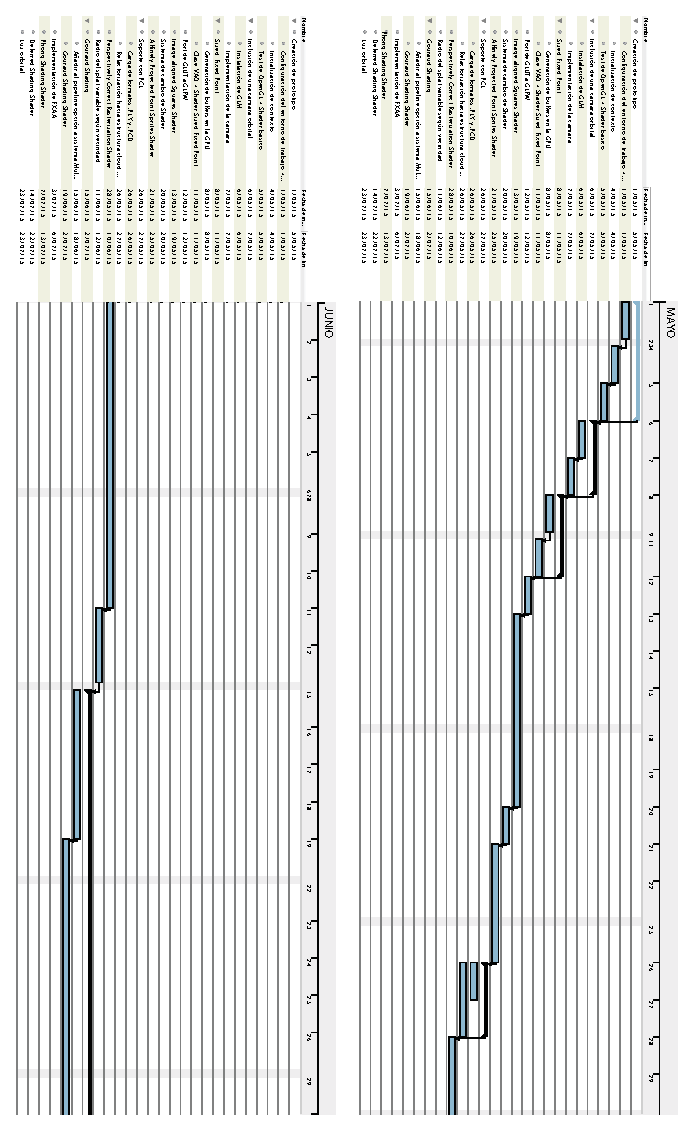
\includegraphics[width=14cm]{../figures/gantt_part1.eps}
        \caption{Diagrama de Gant (I).}
	\label{figure_gantt_part1}
\end{figure}

\begin{figure}
	\centering
	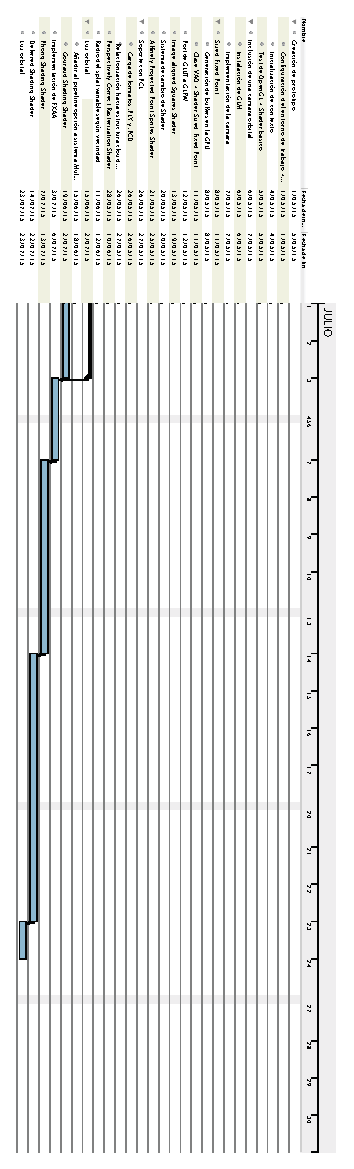
\includegraphics[width=6.72cm]{../figures/gantt_part2.eps}
        \caption{Diagrama de Gant (II).}
	\label{figure_gantt_part2}
\end{figure}

Se tiene adem�s un presupuesto (ver Tabla \ref{presupuesto}) para un proyecto como este. Incluyendo �nicamente costes humanos y \textit{hardware}, ya que el \textit{software} fue siempre gratuito. El precio por hora del ordenador fue calculado pensando en una amortizaci�n de 5 a�os fiscales para el equipo. \\

\begin{table}
\centering
\begin{tabular}{l c c c c}
	\toprule
	\textbf{Recurso} & \textbf{Cantidad} & \textbf{Horas} & \textbf{Coste por hora} & \textbf{Total} \\\midrule
	Software & & & & 0\officialeuro \\
	Ordenador & 1 & 480 & 0,1372\officialeuro & 65,86\officialeuro \\
	Analista-Programador & 1 & 480 & 15\officialeuro & 7200\officialeuro \\\cmidrule(lr){5-5}
	& & & & 7265,86\officialeuro \\
	\bottomrule
\end{tabular}
\caption{Estimaci�n de coste.}
\label{presupuesto}
\end{table}


%
% FIN DEL CAP�TULO
%

	%
% FUNDAMENTOS TECNOL�GICOS
%
\chapter[Fundamentos tecnol�gicos]{
	Fundamentos tecnol�gicos
	\label{nombre_referencia_al_capitulo_020}
}

En este cap�tulo se explicar�n los fundamentos tecnol�gicos necesarios para la comprensi�n de este proyecto. Empezando por la explicaci�n de las Nubes de puntos (ver \ref{s_nubes}), OpenGL (ver \ref{s_opengl}) y la librer�a PCL (ver \ref{s_pcl}).


%
% SECCION - Render de puntos
%
\section[Nubes de puntos]{
	Nubes de puntos
	\label{s_nubes}
}

Una nube de puntos es un conjunto de puntos en un sistema de coordenadas tridimensional. Estos puntos se identifican habitualmente como coordenadas X, Y, y Z y son representaciones de la superficie externa de un objeto.

Las nubes de puntos tienen m�ltiples aplicaciones, entre las que se incluyen la elaboraci�n de modelos tridimensionales en CAD de piezas fabricadas, la inspecci�n de calidad en metrolog�a, y muchas otras en el �mbito de la visualizaci�n, animaci�n, texturizaci�n y aplicaciones de personalizaci�n masiva.

Aunque las nubes de puntos se pueden revisar y texturizar directamente, habitualmente no se utilizan de esta forma en la mayor�a de las aplicaciones tridimensionales, ya que se convierten en modelos de mallas poligonales o mallas triangulares irregulares, modelos de superficie \textit{NURBS}, o modelos de \textit{CAD} mediante un proceso denominado reconstrucci�n de superficies.

Una aplicaci�n en la que las nubes de puntos se utilizan directamente es la metrolog�a y en la inspecci�n industrial (ver Figura \ref{figure_desviaciones}). La nube de una pieza fabricada se alinea a un modelo CAD (o a otra nube de puntos) y se comparan para verificar las diferencias. �stas se visualizan como mapas de color que proporcionan un indicador visual de la desviaci�n entre la pieza fabricada y el modelo CAD. Las dimensiones geom�tricas y tolerancias tambi�n se pueden extraer directamente de la nube de puntos.
\begin{figure}
	\centering
	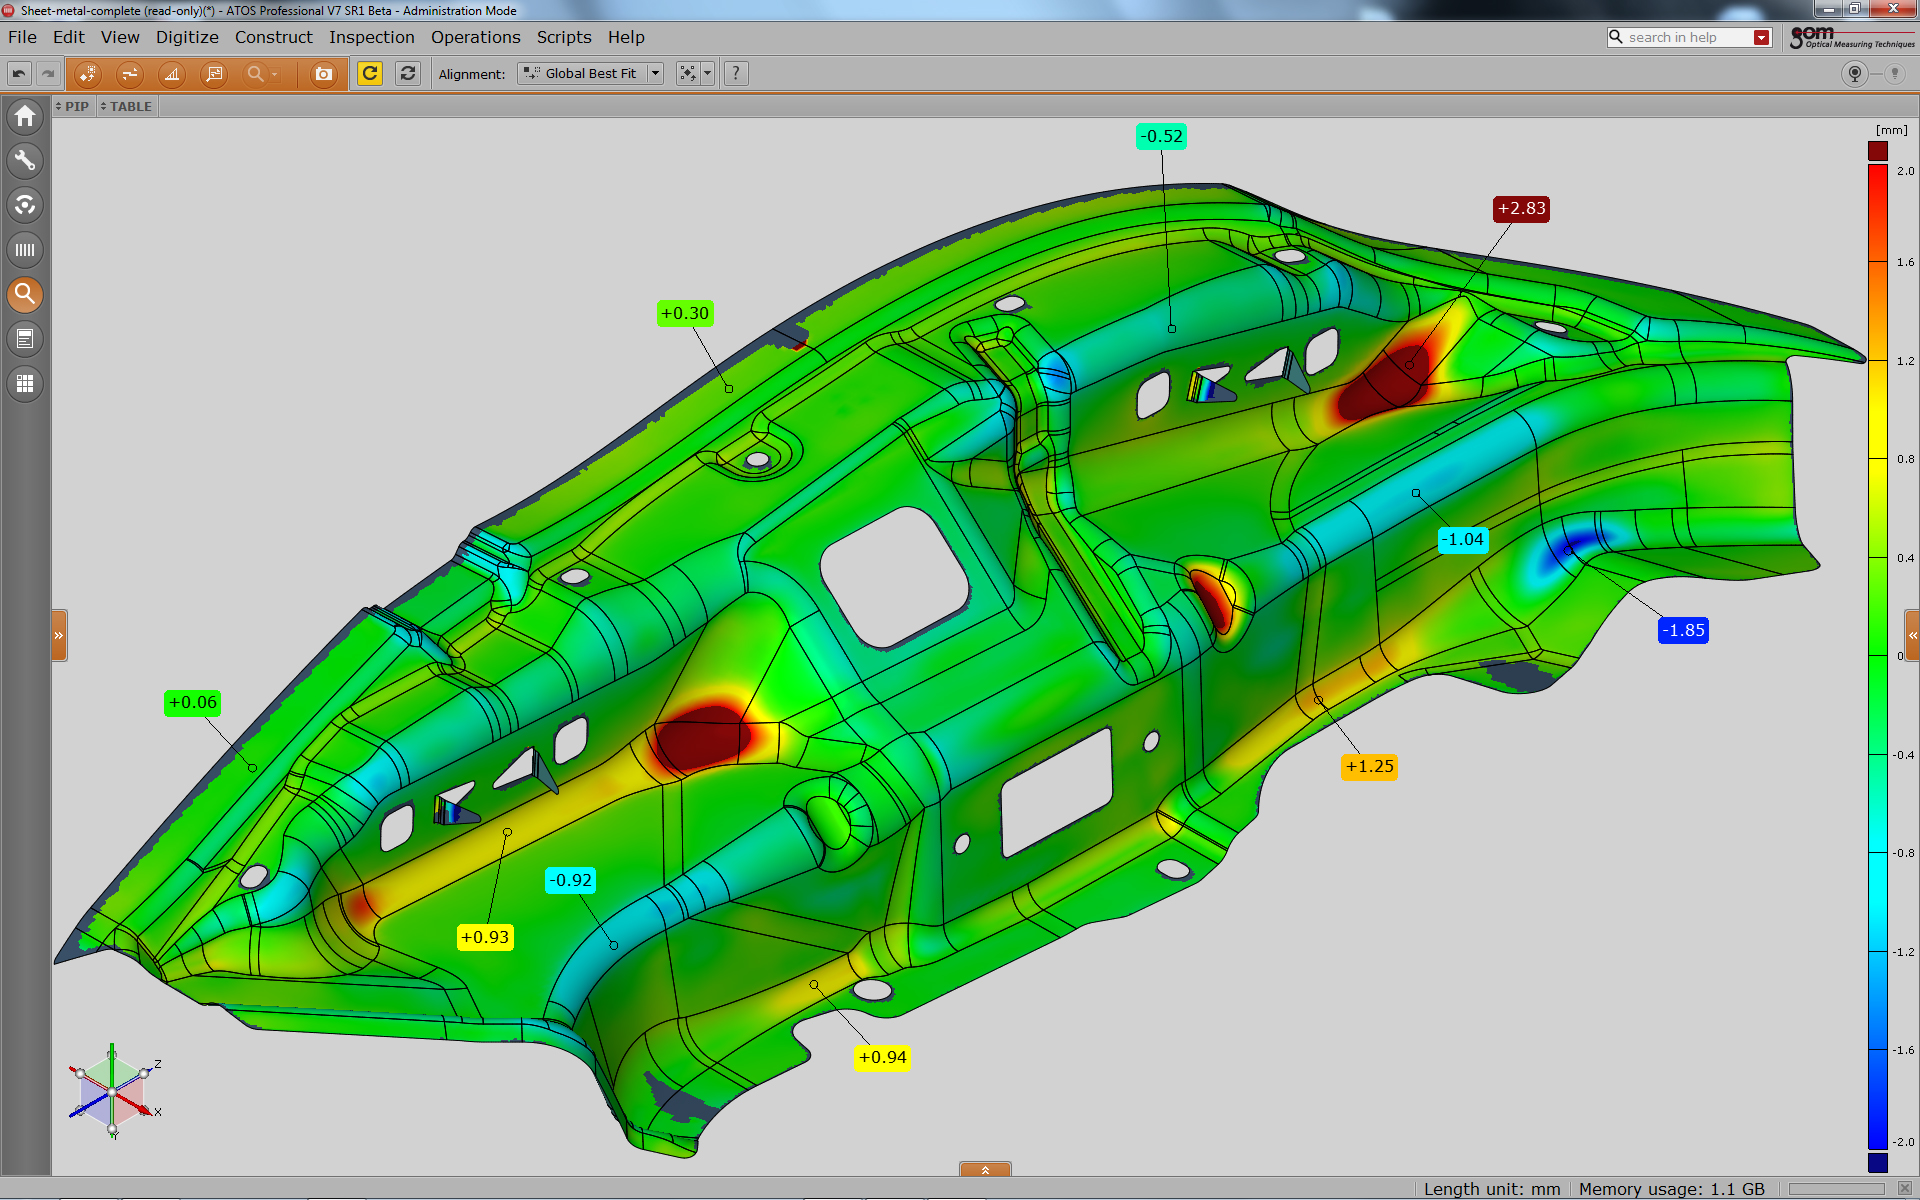
\includegraphics[width=\textwidth]{../figures/gom.jpg}
	\caption{Mapa de desviaciones de una pieza con respecto a un modelo \textit{CAD} en un proceso industrial.}
	\label{figure_desviaciones}
\end{figure}

Las nubes de puntos tambi�n se pueden utilizar para representar datos volum�tricos como en la imagen m�dica. Se logra usando nubes de puntos de muestreo m�ltiple y compresi�n de datos.

En los Sistemas de Informaci�n Geogr�fica \textit{GIS} las nubes de puntos son una de las fuentes de datos para construir modelos digitales del terreno.

\subsection[Adquisici�n] {Adquisici�n}

Para la adquisici�n de estas nubes de puntos, existen actualmente diferentes m�todos:

\begin{itemize}
	\item \textbf{Escaner 3D} Un esc�ner 3D es un dispositivo que analiza un objeto o una escena para reunir datos de su forma y ocasionalmente su color. Diferenciando dos tipos de esc�neres en funci�n de si existe contacto con el objeto o no y  dividiendo estos �ltimos en otras dos categor�as (activos y pasivos).
	
	\begin{itemize}
		\item \textbf{Contacto} Los esc�neres 3D examinan el objeto apoyando el elemento de medida (palpador) sobre la superficie del mismo, t�picamente una punta de acero duro o zafiro. Una serie de sensores internos permiten determinar la posici�n espacial del palpador. Se usan en su mayor�a en control dimensional en procesos de fabricaci�n y pueden conseguir precisiones t�picas de 0,01 mm. 
		
		\item \textbf{Sin contacto}
		\begin{itemize}
			\item \textbf{Activos} Los esc�neres activos (ver Figura \ref{figure_leica}) emiten alguna clase de se�al y analizan su retorno para capturar la geometr�a de un objeto o una escena. Se utilizan radiaciones electromagn�ticas (desde ondas de radio hasta rayos X) o ultrasonidos.
			
			\item \textbf{Pasivos} Los esc�neres pasivos no emiten ninguna clase de radiaci�n por s� mismos, pero en lugar se f�a de detectar la radiaci�n reflejada del ambiente. La mayor�a de los esc�neres de este tipo detectan la luz visible porque es una radiaci�n ya disponible en el ambiente. Otros tipos de radiaci�n, tal como el infrarrojo podr�an ser utilizados tambi�n. Los m�todos pasivos pueden ser muy baratos, porque en la mayor�a de los casos estos no necesitan \textit{hardware} particular.
		\end{itemize}
	\end{itemize}
	
	
	\item \textbf{Fotogrametr�a} La fotogrametr�a es una t�cnica para determinar las propiedades geom�tricas de los objetos y las situaciones espaciales a partir de im�genes fotogr�ficas. B�sicamente, es una t�cnica de medici�n de coordenadas 3D, que utiliza fotograf�as u otros sistemas de percepci�n remota junto con puntos de referencia, como medio fundamental para la medici�n.
\end{itemize}


\begin{figure}
	\centering
	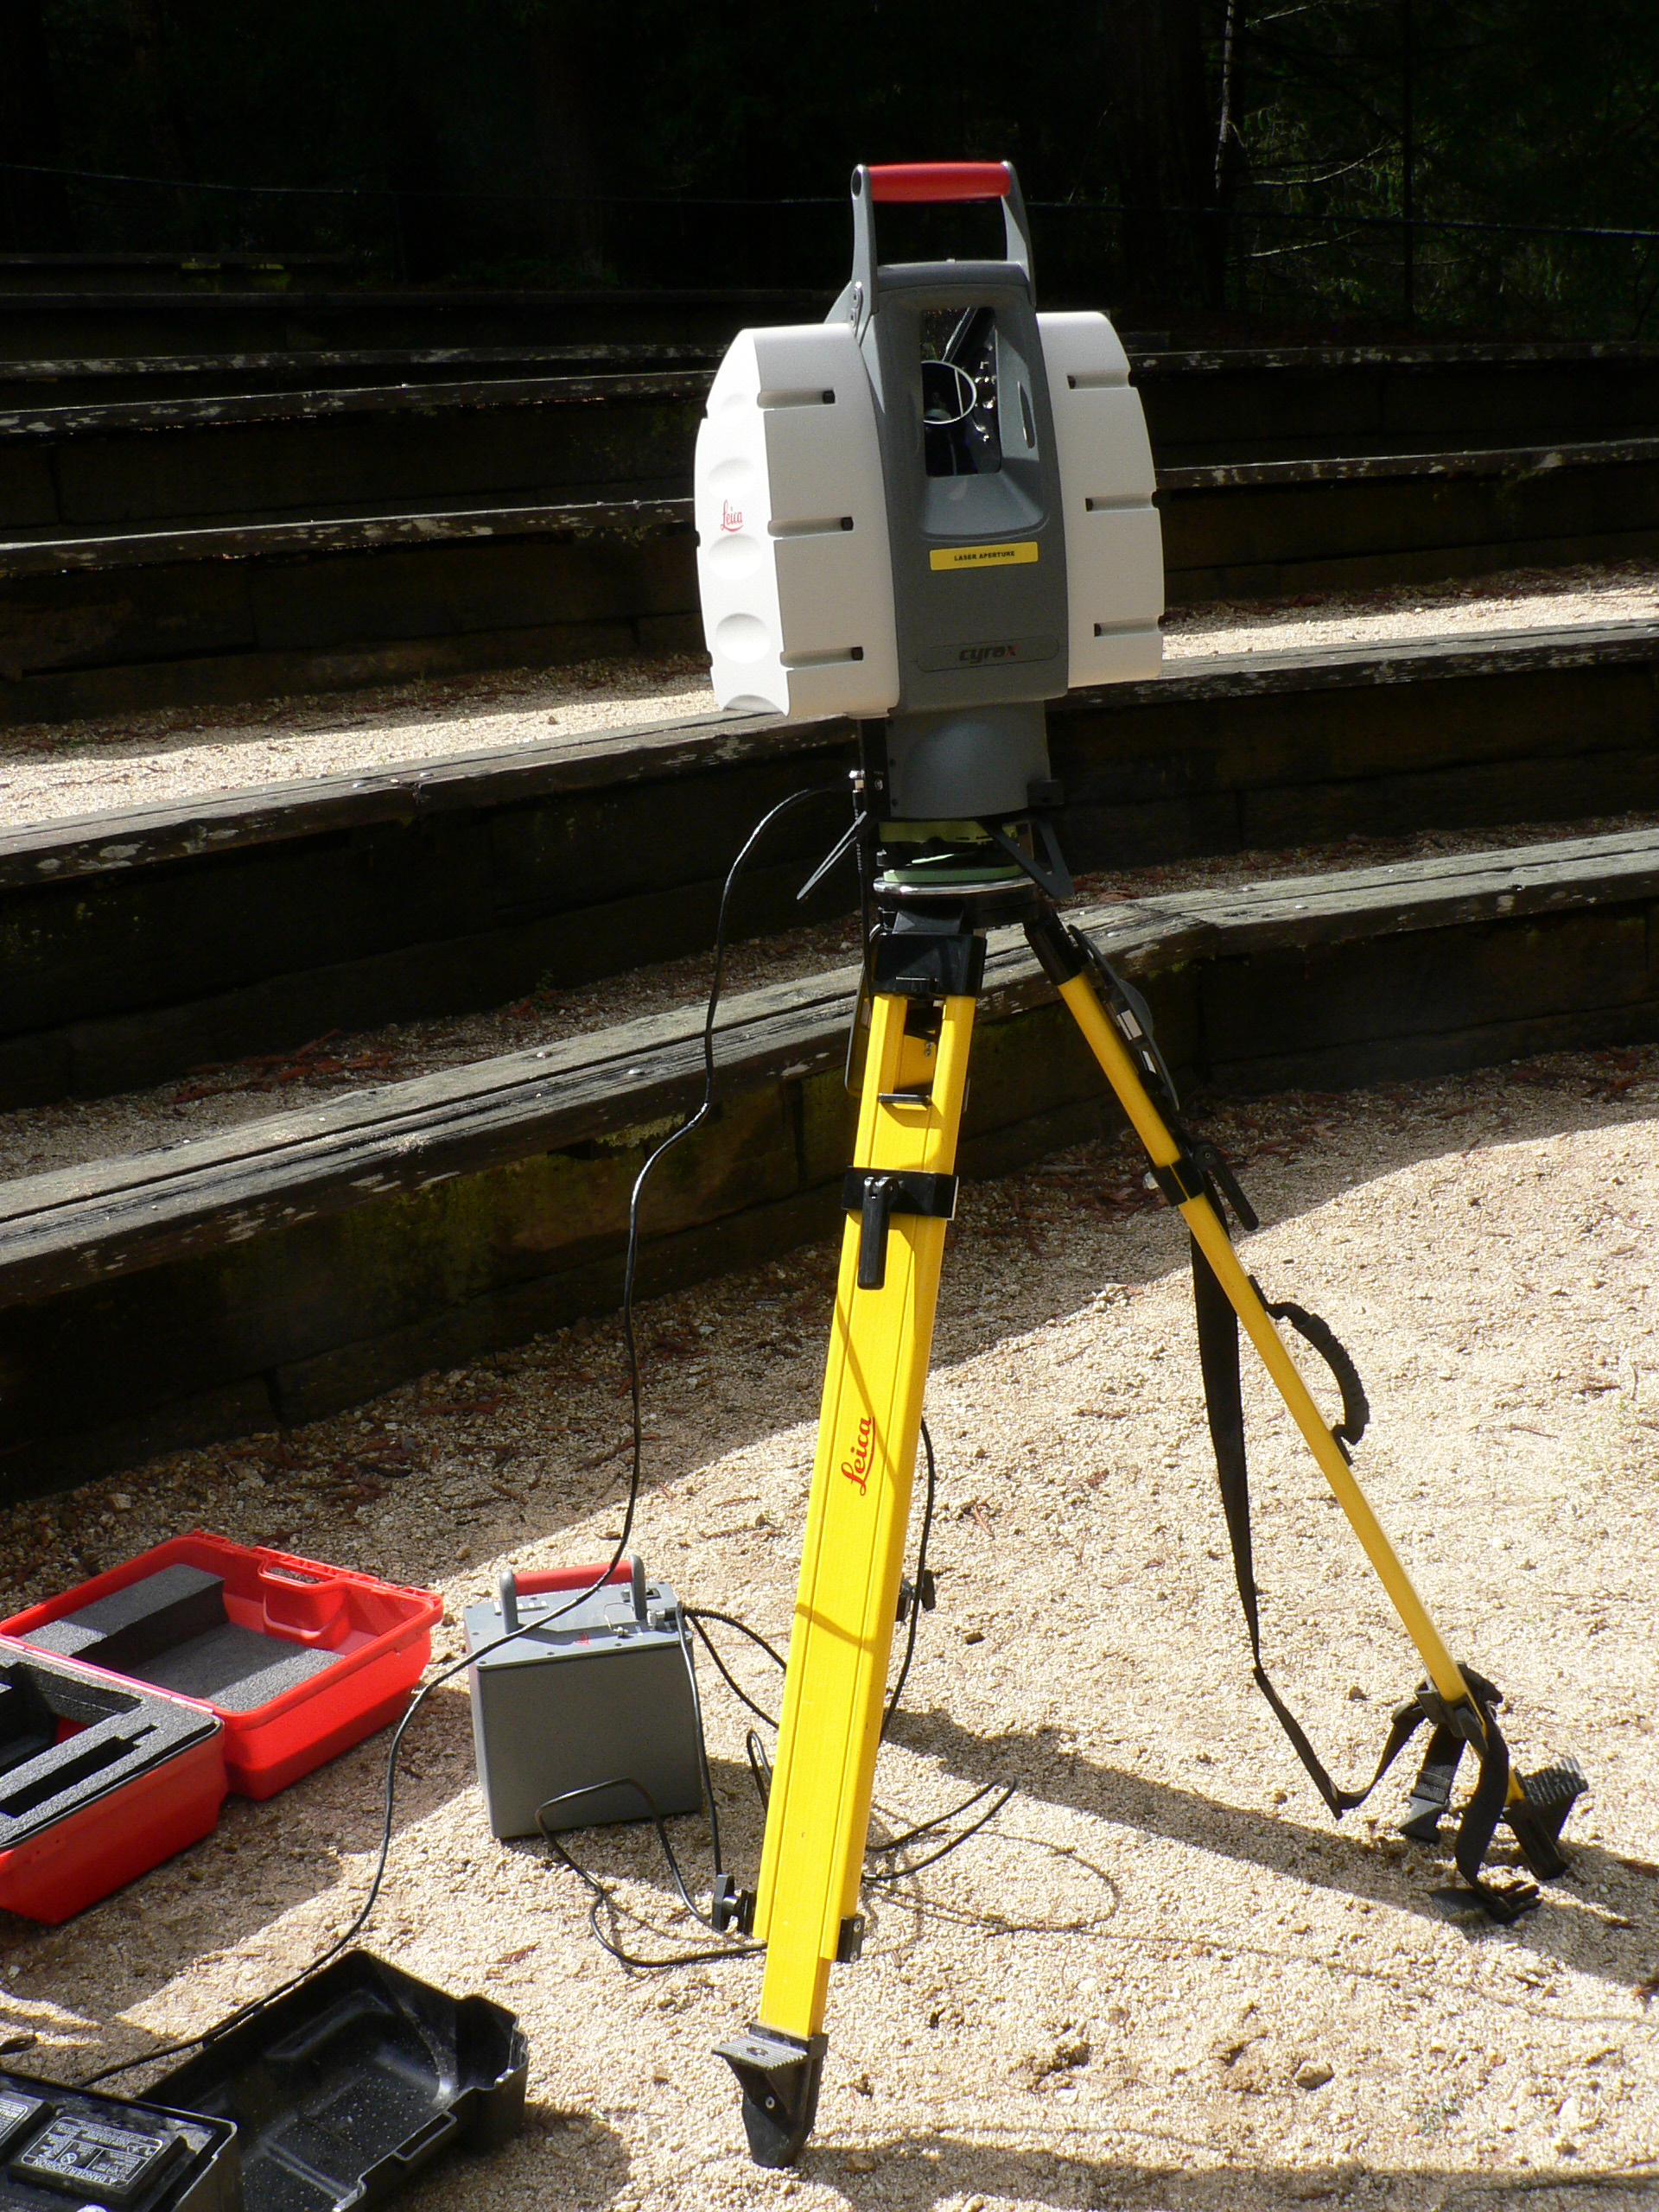
\includegraphics[width=7cm]{../figures/lidar.jpg}
	\caption{Estaci�n Leica LIDAR utilizado para el escaneo de edificios, formaciones rocosas, etc. con el objetivo de generar modelos 3D.}
	\label{figure_leica}
\end{figure}


%
% SECCION - OpenGL
%
\section[OpenGL]{
	OpenGL
	\label{s_opengl}
}

OpenGL (Open Graphics Library) es una libreria multiplataforma destinada a renderizado 2D y 3D. Esta API es t�picamente usada para trabajar con la Unidad Gr�fica de Procesado (GPU) para conseguir un renderizado acelerado mediante \textit{hardware}, aunque es posible que esta sea implementada enteramente mediante \textit{software}.

% Subsecci�n
\subsection[Pipeline] {Pipeline}

El \textit{Pipeline} de render es una secuencia de pasos funcionales para la obtenci�n de im�genes de escenas 3D. Idealmente, si se divide un proceso en $ n $ etapas se incrementar� la velocidad del proceso en ese factor $ n $. As�, la velocidad de la cadena viene determinada por el tiempo requerido por la etapa m�s lenta. 

El \textit{pipeline} que OpenGL sigue en la renderizaci�n de objetos (ver Figura \ref{figure_opengl_pipeline}) ser�a el siguiente:

\begin{enumerate}
	\item Preparaci�n del \textit{Vertex Array Object} a renderizar.
	
	\item Procesamiento de los v�rtices:
	\begin{enumerate}
		\item  Cada v�rtice del flujo de datos (\textit{stream}) es procesado mediante el \textit{vertex shader} con motivo de realizar las transformaciones necesarias de estos a un espacio de coordenadas adaptado a su proyecci�n.
		
		\item Fase opcional de teselaci�n.
		
		\item Fase opcional \textit{geometry shader}. La salida es una secuencia de primitivas.
	\end{enumerate}
	
	\item \textit{Vertex Post-Processing}, la salida del anterior paso es ajustado (\textit{primitive clipping} y transformaci�n del \textit{viewport} a coordenadas de la ventana). 
	
	\item \textit{Primitive Assembly}.
 	
	\item Las primitivas son divididas en elementos discretos, los cuales generan un numero determinado de fragmentos.
	
	\item El \textit{fragment shader} procesa cada fragmento generando un numero diferente de salidas.
	
	\item \textit{Per-Sample Processing}, donde se descartan fragmentos, se combinan los colores de los fragmentos obtenidos del \textit{fragment shader} con los que ya existen en el \textit{buffer}, ademas de realizar diferentes operaciones l�gicas.

\end{enumerate}

\begin{figure} [H]
	\centering
	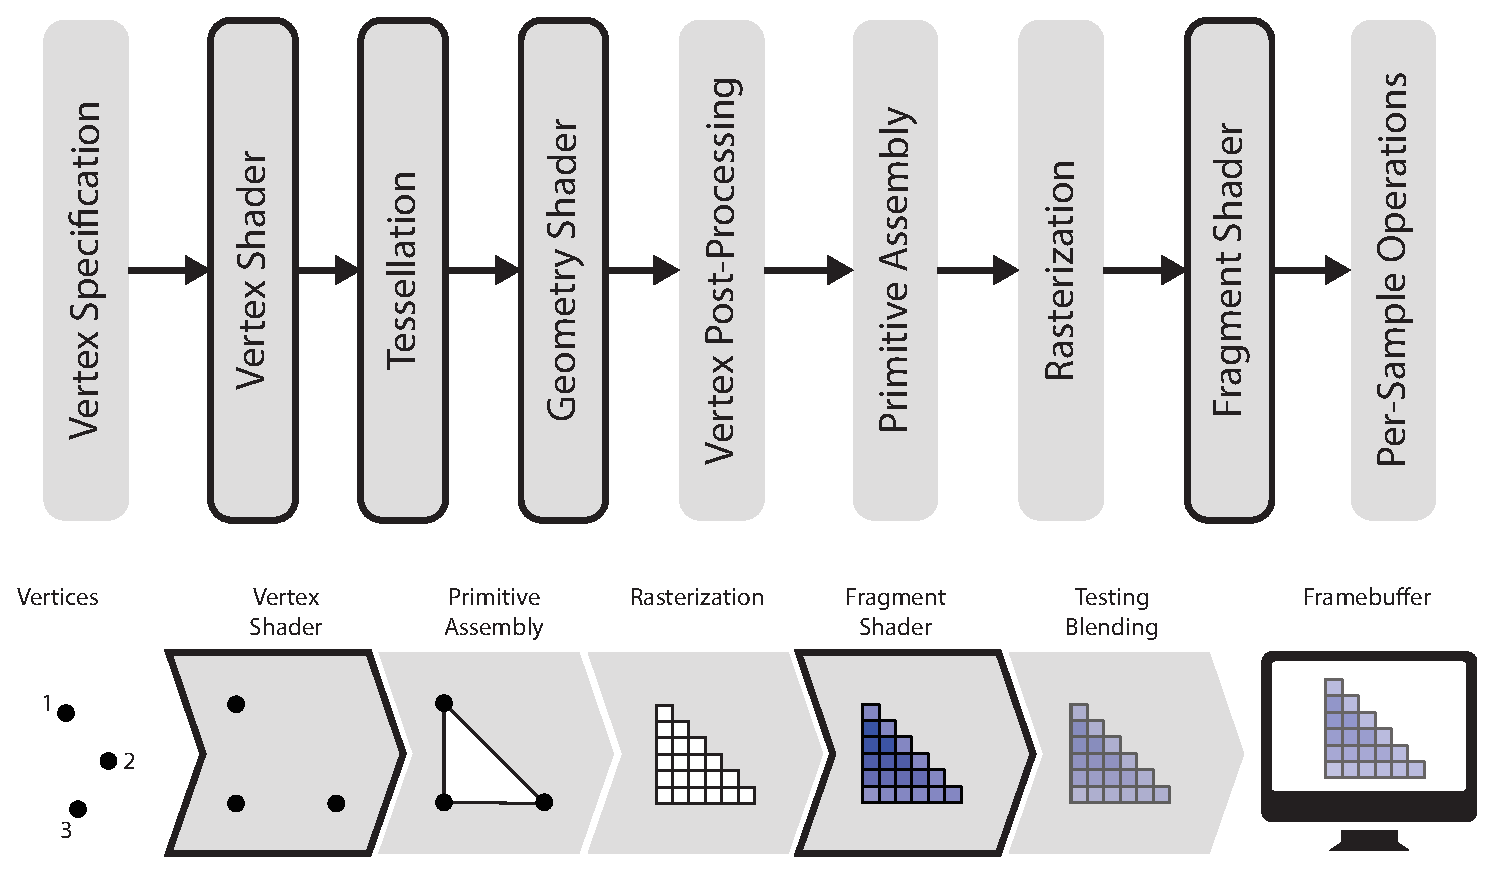
\includegraphics[width=\textwidth]{../figures/pipeline.eps}
	\caption{El pipeline de OpenGL, las fases es negrita son programables.}
	\label{figure_opengl_pipeline}
\end{figure}

\subsection[Shaders] {Shaders}

El \textit{hardware} de aceleraci�n gr�fica ha sufrido una importante transformaci�n en la �ltima d�cada. Como se muestra en la Figura \ref{figure_evolucion_gpu}, en los �ltimos a�os el potencial de las \textit{GPUs} ha superado con creces al de la \textit{CPU}.

Esta tendencia en el \textit{hardware} gr�fico ha reemplazado la funcionalidad fija del antiguo \textit{pipeline} con areas programables mediante peque�os programas. De este modo algunas de las fases del \textit{pipeline} pueden ser modificadas con peque�os programas escritos por el usuario denominados \textit{shaders}. Estos programas se ejecutan directamente en la \textit{GPU}, y permite realizar operaciones a diferentes niveles con alta eficiencia.

El lenguaje de OpenGL de \textit{Shading} (\textit{GLSL}) est� basado en ANSI C y muchas de las caracter�sticas han sido mantenidas excepto las que entraban en conflicto con temas de rendimineto o implementaci�n. C fu� extendido con tipos nuevos para manejar estructuras como vectores o matrices, para hacer mas f�cil operaciones t�picas en gr�ficos 3D. 

En al figura \ref{figure_opengl_pipeline} se puede observar que en OpenGL las fases referentes al \textit{vertex shader}, \textit{tessellation}, \textit{geometry shader} o \textit{fragment shader} pueden ser programables.

\begin{figure}
	\centering
	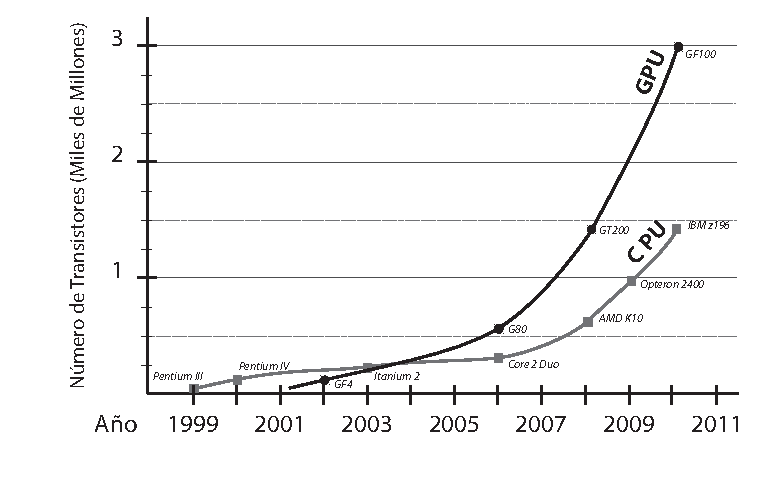
\includegraphics[width=\textwidth]{../figures/integracion-transistores.eps}
	\caption{Evoluci�n del n�mero de transistores en GPU y CPU (1999 - 2010).}
	\label{figure_evolucion_gpu}
\end{figure}

%
% SECCION - PCL
%
\section[PCL]{
	PCL
	\label{s_pcl}
}
\textit{Point Cloud Library} (\textit{PCL}) es una librer�a \textit{open-source} con algoritmia destinada a tareas de  procesamiento de nubes de puntos y geometr�a 3D. La librer�a contiene algoritmos para estimaci�n, reconstrucci�n de superficies, \textit{model fitting} y segmentaci�n. Est� escrita en C++ y distribuida bajo una licencia \textit{BSD}.

Estos son usandos, por ejemplo, para percepci�n en rob�tica para filtrar ruido, unir nubes de puntos 3D, extraer \textit{keypoints} y calcular descriptores para reconocimiento de objetos basados en su geometr�a y crear superficies a partir de nubes de puntos para visualizarlas.

El desarrollo de esta librer�a comenz� en Marzo de 2010 
The development of the Point Cloud Library started in March 2010 en la empresa \textit{Willow Garage}. La primera version oficial de \textit{PCL} fue lanzada en Mayo de 2011.

%
% FIN DEL CAP�TULO
%
	%
% VISUALIZACI�N DE NUBES DE PUNTOS
%
\chapter{
	Fundamentos de la Programaci�n Gr�fica
	\label{nombre_referencia_al_capitulo_030}
}

En este cap�tulo se introducen algunos conceptos b�sicos de
inform�tica gr�fica, en especial los relativos a los fundamentos
detr�s de la obtenci�n de un \textit{render} 3D.


%
% SECCION - Render
%
\section[Render]{
	Render
	\label{s_render}
}

Tradicionalmente la Programaci�n Gr�fica ha sido definida como la disciplina dedicada a sintetizar im�genes algoritmicamente mediante ordenadores~\cite{foley}. Actualmente se pueden encontrar mas temas acerca del hiper realismo, t�cnicas de animaci�n, realidad virtual, etc. Para generar im�genes a partir de escenas tridimensionales un proceso denominado \textit{render} es usado. Este conjunto de acciones est� al cargo del modelado y sus propiedades, iluminaci�n y si es necesario la c�mara que capturar� todo.

Como bien se dijo antes, el \textit{render} es el proceso computacional de generar una imagen a partir de un modelo. Desde esta definici�n, se podr�a sacar diferentes interpretaciones, desde crear una pel�cula de animaci�n 3D a un diagrama de barras, y todas ellas ser�an igualmente v�lidas. Aunque el t�rmino que normalmente es usado es referido a un modelo tiene una naturaleza espacial y mas espec�ficamente tridimensional

Diferentes clasificaciones de t�cnicas de \textit{render} puede ser definidas, pero para esta introducci�n usaremos dos de ellas. Por un lado, si nos fijamos en el estilo de la imagen que se pretende conseguir:

\begin{itemize}
	\item \textbf{Fotoreal�stico} que intenta ser lo m�s fiel como sea posible a la realidad. Este tipo de \textit{render} puede ser subdivido en:
	\begin{itemize}
		\item \textbf{Render basado en F�sicas} Intentando calcular una simulaci�n lo m�s aut�ntica posible del tratamiento de la luz a trav�s de la escena y su interacci�n con materiales y objetos. La precisi�n de la simulaci�n depender� de los modelos f�sicos y matem�ticos escogidos.
		
		\item \textbf{Falseados} que utiliza trucos para reducir tiempos de renderizado.
	\end{itemize}
	
	\item \textbf{No fotoreal�sticos} que pretende usar otros tipos de efectos para la renderizaci�n de la escena con motivos art�sticos.
\end{itemize}

La Figura \ref{figure_comparacion_render} muestra la diferencia entre ambas aproximaciones.

\begin{figure}
	\centering
	\includegraphics[width=\textwidth]{../figures/realistic_vs_non.eps}
	\caption{Fotorealistic (izquierda) vs. No fotoreal�sticos (derecha).}
	\label{figure_comparacion_render}
\end{figure}

Por otro lado, si se comparan las opciones de interacci�n de la aplicaci�n con el usuario final, se podr�a dividir las t�cnicas en 2 apartados:
\begin{itemize}
	\item \textbf{Render Offline} Donde el proceso de generar la imagen es demasiado lento para responder instant�neamente a las interacciones del usuario, en general por la b�squeda de un resultado realista~\cite{pbrt}. Una escala de tiempo de segundos a incluso d�as podr�a considerarse �lento�. Esto ocurre por ejemplo cuando se generan fotogramas para una pel�cula.
	
	\item \textbf{Render Online, Real-time o Interactivo} Donde el tiempo para la obtenci�n de las im�genes es suficientemente corto como para responder a la interacci�n del usuario en la aplicaci�n~\cite{rtr}, teniendo este una sensaci�n de continuidad. Una escala de \textit{milisegundos} tendr�a que ser alcanzada para obtener este efecto. Normalmente medida en \textit{frames per second} (FPS). Un buen ejemplo de este grupo podr�an ser los videojuegos.
\end{itemize}

La mayor parte del trabajo realizado en este documento se ha centrado en la obtenci�n de un render interactivo, lo que en general implica sacrificar muchos aspectos presentes en una aproximaci�n fotoreal�stica.


\subsection[Modelos 3D]{Modelos 3D}

El modelado describe el proceso de formar la figura de un objeto virtual en un ordenador. Existen realmente tres tipos diferentes de Modelos 3D:
	
\begin{itemize}
	\item \textbf{Basado en Pol�gonos:} Donde se describe la superficie de un objeto mediante un conjunto de pol�gonos. La forma triangular es la mas comunmente usada para esta tarea, puesto que son planos y trivialmente convexos. Pr�cticamente la totalidad del \textit{hardware} gr�fico esta optimizado pensando en esta primitiva.
	
	Aunque en el proceso del modelado de un objeto, este no tiene porque estar construido usando tri�ngulos. En �ltima instancia, es convertido a un conjunto de tri�ngulos mediante un proceso conocido como teselaci�n.
	
	\item \textbf{Basado en Voxels:} Divide el espacio tridimensional en una rejilla donde el \textit{voxel} es la m�nima unidad de medida. Cada una de estas celdas es rellenada o no, dependiendo de si se pretende que sea renderizada. La memoria necesaria aumenta en funci�n de la precisi�n necesaria. Este tipo de procesos usualmente utilizado en Inform�tica Biom�dica.
	
	\item \textbf{Basada en Puntos:} Los objetos son representados mediante puntos que son producto de un muestreo de su superficie. Cada punto tiene una posici�n y alguna informaci�n relativa a la superficie a la que pertenece. Comparado con el modelo tradicional basado en pol�gonos esta primitiva necesita sus propias t�cnicas de \textit{render}. Este es nuestro caso de estudio.
	
\end{itemize}


\section[Espacios 3D y transformaciones]{Espacios 3D eucl�deos y transformaciones}

En gr�ficos por computaci�n normalmente trabajamos con espacios tridimensionales de geometr�a Eucl�dea. El t�rmino �Eucl�deo� es usado para distinguir estos espacios y los espacios curvos de geometr�a no Eucl�dea. Las operaciones mas t�picas en geometr�a Eucl�dea puede ser representada con matrices de transformaci�n si se usan sistemas de coordenadas homog�neos~\cite{foley}. Debido a esto una transformaci�n \textbf{T} puede ser usada para diferentes motivos.

Usando conceptos b�sicos de �lgebra lineal, una matriz $4 \times 4$ puede ser usada para expresar transformaciones lineales de un punto o un vector. Una transformaci�n entonces ser� representada por los elementos de la matriz $4 \times 4$. Ellas puede ser tambi�n usadas para realizar algunas transformaciones no lineales en espacios Eucl�deos. Por esta raz�n, las matrices de transformaci�n son altamente usadas en esta disciplina.

Generalmente una transformaci�n es una funci�n de puntos a puntos o vectores a vectores, por ejemplo:
 \begin{equation}p' = \textbf{T}(p) \;\;\;\;\; v' = \textbf{T}(v)\end{equation} 

Para transformar los puntos o vectores simplemente se tiene que realizar las apropiadas multiplicaciones de matrices. Esto tambi�n permite la composici�n de transformaciones, multiplicando las matrices de transformaci�n.

Las transformaciones mas utilizadas comunmente son:
\begin{itemize}
	\item \textbf{Rotaci�n}, con el que se podr� rotar un punto o vector seg�n un �ngulo dado alrededor de un eje arbitrario o los ejes $x$, $y$ o $z$.
	\item \textbf{Escalado}, para un punto o vector dado, esta transformaci�n escalar� los componentes $x$, $y$ y $z$ por un factor.
	\item \textbf{Translaci�n}, �nicamente afecta a puntos y podr� transladar las coordenadas $x$, $y$ y $z$ una cantidad.
	\item \textbf{Modelo}, esta matriz es �til para transformaciones del modelo localmente. De estar compuesto por un conjunto de matrices de rotaci�n, escalado o translaci�n. Cuando sea aplicada esta matriz a todos los puntos, los tendremos en coordenadas del mundo. 
	\item \textbf{Vista}, inicialmente la c�mara es localizada en el origen del espacio mundo. Para poder moverla alrededor del espacio mundo esta matriz es utilizada. Esta matriz tambi�n es denominada como ``mirar a''. Luego de que esta transformaci�n sea aplicada, tendremos los puntos en coordenadas de la c�mara.
	\item \textbf{Proyecci�n}, puesto que la escena tiene que ser proyectada tanto en una pantalla como en una imagen 2D, necesitamos otro proceso que convierta los puntos desde las coordenadas de la c�mara a coordenadas homog�neas de modo que estas puedan ser proyectadas en pantalla.
\end{itemize}

Normalmente la composici�n de las matrices del modelo, vista y proyecci�n es llamado \textit{MVP} y es aplicada a cada punto que queramos dibujar.

Para ilustrar como las transformaciones son representadas por una matriz $4 \times 4$, la ecuaci�n \ref{eq_trans} muestra la matriz gen�rica para la translaci�n:
\begin{equation}\label{eq_trans}\textbf{T}(\Delta x,\Delta y,\Delta z) = \begin{pmatrix}
1& 0 & 0 & \Delta x\\ 
0& 1 & 0 & \Delta y\\ 
0& 0 & 1 & \Delta z\\ 
0& 0 &0  & 1
\end{pmatrix}\end{equation}

Esta transformaci�n es aplicada al punto $P=(x,y,z)$ de la siguiente forma:
\begin{equation}\begin{pmatrix}
1& 0 & 0 & \Delta x\\ 
0& 1 & 0 & \Delta y\\ 
0& 0 & 1 & \Delta z\\ 
0& 0 & 0 & 1
\end{pmatrix} \begin{pmatrix}
x\\
y\\
z\\ 
1
\end{pmatrix} = \begin{pmatrix}
x+\Delta x\\
y+\Delta y\\
z+\Delta z\\ 
1
\end{pmatrix}\end{equation}


\section{Camera model}\label{camera_model}

Casi todo el mundo actualmente ha usado una c�mara y conoce su prop�sito: se quiere obtener una imagen del mundo (normalmente presionando un bot�n) y la imagen es entonces almacenada en un \textit{film}. Una de las c�maras mas simples es la c�mara estenopeica. Este tipo de c�maras est�n compuestas por: una caja estanca, un peque�o orificio por donde entra la luz (estenopo) y un material fotosensible. De modo que cuando el peque�o orificio es descubierto la luz entra a trav�s de el y alcanza la pieza de material fotosensible que est� dispuesto al otro lado de la caja (ver Figura \ref{figure_pinhole_camera}). Hoy en d�a, las c�maras son mucho mas complejas de funcionamiento que esta simple c�mara, pero es un buen comienzo para explicar como el funcionamiento de nuestra simulaci�n.\\

\begin{figure} [H]
	\centering
	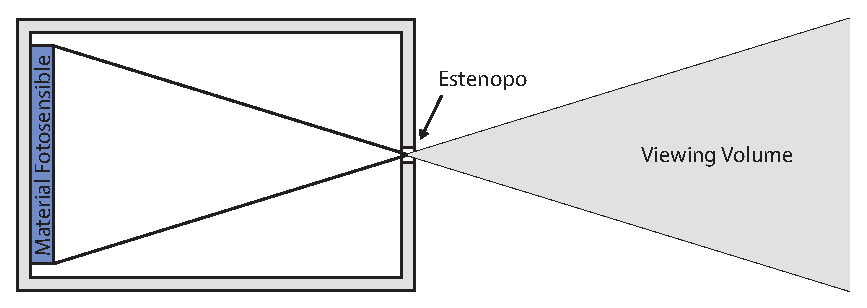
\includegraphics[width=12 cm]{../figures/camara_estenoscopica.eps}
	\caption{Funcionamiento de una c�mara estenopeica.}
	\label{figure_pinhole_camera}
\end{figure}

Lo m�s importante es definir que parte de la escena ser� reflejada en el papel fotosensible. Conectando el estenopo con las aristas del papel se genera una doble pir�mide que extiende dentro de la escena. Los objetos que que no estean dentro de esta pir�mide no quedar�n reflejados en la im�gen del film. Como las c�maras de hoy en dia son mas complejas, se referir� a la regi�n que puede ser reflejada en la imagen final como \textit{viewing volume}.

Puesto que la im�gen obtenida es la situada enfrente de el estenopo, este comunmente es tambi�n referido como \textit{ojo}. Una cantidad de luz viajar� del mundo al plano donde est� situado el material fotosensible. Varios tests ser�n realizados por OpenGL dependiendo del tipo de c�mara para establecer que puntos pueden ser vistos y tendr�n que ser representados en el \textit{frame-buffer}.

El modelo de la c�mara usado en este proyecto soporta diferentes configuraciones. Primero se explicar� como estos par�metros afectan al modelo de la c�mara, luego se explicar� como el modelo interacciona con el proceso de \textit{ray tracing}. 

\subsection{Par�metros de la c�mara}

El primer par�metro que el modelo de la c�mara soporta es la \textbf{posici�n}. Este par�metro establece donde la c�mara tendr� que estar situada en el espacio de coordenadas del mundo (\textit{x,y,z}). 

El siguiente par�metro soportado es el de la rotaci�n. Este par�metro es un punto en el mundo hacia donde la c�mara estar� mirando.
Tambi�n necesitamos saber c�mo orientar la c�mara a lo largo de la direcci�n de visi�n impl�cita por los dos primeros par�metros .

Tambi�n es necesario conocer como est� orientada la c�mara con respecto a la direcci�n en la que se est� mirando implicado por los 2 primeros par�metros. El par�metro \textit{vector up} nos da esa orientaci�n.

Otros par�metros importantes en el modelo de la c�mara son los planos de \textit{clipping}, que nos dar�n el rango a lo largo del eje \textit{z} que dejar� que los objetos dentro de el sean renderizados. \textbf{Near} establece la posici�n del plano cercano y \textbf{far} indica la posici�n del plano de \textit{clipping} lejano.

El �ltimo par�metro que la c�mara soporta es el \textbf{campo de visi�n}. El �ngulo de visi�n describe la extensi�n angular de la escena capturada por la c�mara horizontal y verticalmente .

Los planos de \textit{clipping} y los �ngulos de visi�n define el \textit{viewing volume} en el modelo, tambi�n conocido como \textit{viewing frustum}. 

El usuario tambi�n tiene la opci�n de usar entre una c�mara con proyecci�n \textbf{perspectiva} o \textbf{ortogr�fica} dependiendo de las necesidades. En arquitectura por ejemplo se suele preferir una c�mara ortogr�fica, mientras que un usuario normal suele preferir una en perspectiva puesto que el campo de visi�n da un resultado m�s natural. (ver Figura \ref{figure_diferencia_camara})

\begin{figure} [H]
	\centering
	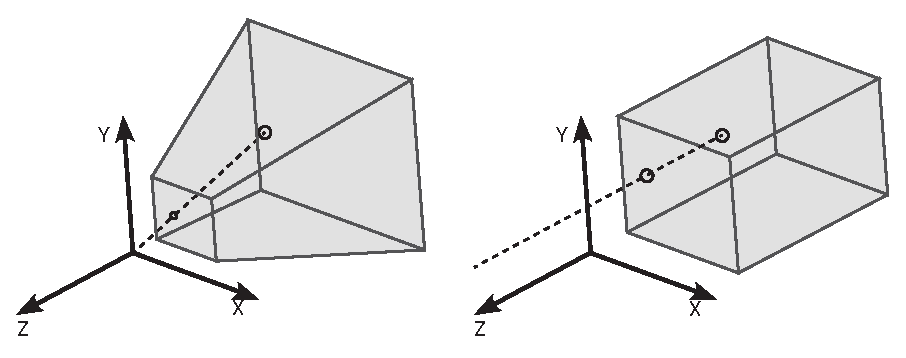
\includegraphics[width=\textwidth]{../figures/orto_and_perspect.eps}
	\caption{Representaci�n de las diferencias entre c�mara en perspectiva (izquierda) y ortogr�fica (derecha).}
	\label{figure_diferencia_camara}
\end{figure}

La proyecci�n ortogr�fica es mas comunmente utilizada en ingenier�a puesto que las dimensiones son mostradas de forma inequ�voca, si hay alguna linea de unidad en cualquier lado de la escena, esta se mostrara con la misma longitud en cualquier lado. Tambi�n cualquier par de lineas que sean paralelas lo ser�n tambi�n en la realidad. Con la proyecci�n en perspectiva, lineas de id�ntico tama�o en la vida real podr�n aparecer de longitud diferente debido al \textit{escorzo}.\footnote{Los objetos se vuelven m�s peque�os en la imagen en cuanto est�n situados en un plano m�s lejano.}. Esto hace que sea dif�cil juzgar las dimensiones relativas de un objeto cuando est� lejano.     

\subsection{Funcionamiento interno de la c�mara}

Una vez que se tienen los par�metros que se necesitan para localizar la c�mara en escena, usaremos una transformaci�n \textit{mirar a} para este prop�sito. Usando esta transformaci�n como matriz de vista nos dar� una transformaci�n entre coordenadas del mundo y la c�mara como se mencion� anteriormente. La matriz es construida usando la posici�n ($p$), orientaci�n ($o$) y \textit{vector up}($u$).

Primero, un vector direcci�n $f$ es construido:
\begin{equation}f = \frac{p - o}{\left \| p - o \right \|}\end{equation}

Despu�s, el vector \textit{right} $r$:
\begin{equation}r = f \times u\end{equation}

Luego, un nuevo vector \textit{up} $u'$ es calculado en funci�n de la referencia de la c�mara:
\begin{equation}u' = r \times f\end{equation}

Con �stos, una matriz de rotaci�n se puede construir lo que representa una reorientaci�n en la base ortonormal de nueva creaci�n:
\begin{equation}R = \begin{bmatrix}
r_{x} & u'_{x} & f_{x} & 0\\ 
r_{y} & u'_{y} & f_{y} & 0\\ 
r_{z} & u'_{z} & f_{z} & 0\\ 
0 & 0 & 0 & 1
\end{bmatrix}\end{equation}

Por �ltimo, para transformar objetos en el marco de la c�mara; no s�lo todo tiene que ser orientada correctamente, sino que tambi�n tiene que ser trasladado desde el origen hasta la posici�n de la c�mara. Esto se logra mediante la concatenaci�n de la matriz de rotaci�n $ R $ con la matriz correspondiente:
\begin{equation}\label{view}V = \begin{bmatrix}
r_{x} & u'_{x} & f_{x} & -p_{x}\\ 
r_{y} & u'_{y} & f_{y} & -p_{y}\\ 
r_{z} & u'_{z} & f_{z} & -p_{z}\\ 
0 & 0 & 0 & 1
\end{bmatrix}\end{equation}

La ecuaci�n \ref{view} es la resultante  matriz \textit{mirar a} \textbf{\textit{V}} que ser� usada para transformar los puntos del espacio mundo a coordenadas de la c�mara.

La siguiente fase depender� del tipo de c�mara que el usuario elija, ortogonal o perspectiva. En funci�n de esta elecci�n una matriz de proyecci�n ser� escogida.

Si es escogida una c�mara perspectiva, tendremos que tener en cuenta el efecto del escorzo mencionado anteriormente. Esta proyecci�n no conserva distancias, �ngulos, y paralelismo entre lineas.\emph{x} e \emph{y} ser�n modificadas de acuerdo al correspondiente valor de \textit{z}, que establece como de cerca a la c�mara est� un punto. Para obtener este efecto, una matriz perspectiva ser� utilizada. Una matriz comunmente utilizada es la matriz \textit{frustum}. En ella el espacio homog�neo obtiene la forma de una pir�mide truncada. Los par�metros usados para la construcci�n de esta matriz ser�an el \textbf{izquierda} ($l$), \textbf{derecha} ($r$), \textbf{arriba} ($t$), \textbf{abajo} ($b$), plano \textbf{near} ($n$) y \textbf{far} ($f$) del \textit{frustum}.

$t$ es obtenida de la siguiente forma usando los par�metros de la c�mara del \textbf{campo de visi�n} ($fov$) y el plano \textit{near} ($n$):
\begin{equation}t = n \cdot tan(fov / 2) \end{equation} 

Luego, $r$ es obtenida usando el ancho ($w$) y alto ($h$) de la ventana:
\begin{equation}r = t \cdot w / h \end{equation}   

Puesto que el \textit{frustum} es sim�trico, $l$ y $b$ ser�n lo mismo que $r$ y $l$ pero de signo opuesto. Una vez se tienen todos los par�metros se podr� construir las matrices de perspectiva u ortogr�fica:
\begin{equation}\label{pers}P = \begin{bmatrix}
\frac{2 \cdot n}{r - l} & 0 & \frac{r + l}{r - l} & 0\\ 
0 & \frac{2 \cdot n}{t - b} & \frac{t + b}{t - b} & 0\\ 
0 & 0 & \frac{n + f}{n - f} & \frac{2 \cdot n \cdot f}{n - f}\\ 
0 & 0 & -1 & 0
\end{bmatrix}\end{equation}

En contraste, si la c�mara requerida es la ortogr�fica, una matriz algo m�s simple se puede usar. Los puntos ser�n proyectados al plano \textit{near}. Este tipo de transformaciones no da el efecto de escorzo, manteniendo paralelas y manteniendo la distancia relativa entre objetos. Esta transformaci�n mantiene \textit{x} e \textit{y} invariables, pero cambia el valor de \textit{z} al plano \textit{near}. Los par�metros para la construcci�n de esta matriz son tambi�n \textbf{izquierda} ($l$), \textbf{derecha} ($r$), \textbf{arriba} ($t$), \textbf{abajo} ($b$) y plano \textbf{near} ($n$) del \textit{frustum}:
\begin{equation}\label{ortho}P = \begin{bmatrix}
\frac{2}{r - l} & 0 & 0 &  \frac{l + r}{l - r}\\ 
0 & \frac{2}{t - b} & 0 & \frac{b + t}{b - t}\\ 
0 & 0 & \frac{2}{n - f} & \frac{n + f}{f - n}\\ 
0 & 0 & 0 & 1
\end{bmatrix}\end{equation}

Una de estas dos matrices (\ref{pers} or \ref{ortho}) representar�n la matriz de proyeccion \textbf{\textit{P}}.

\begin{figure} [H]
	\centering
	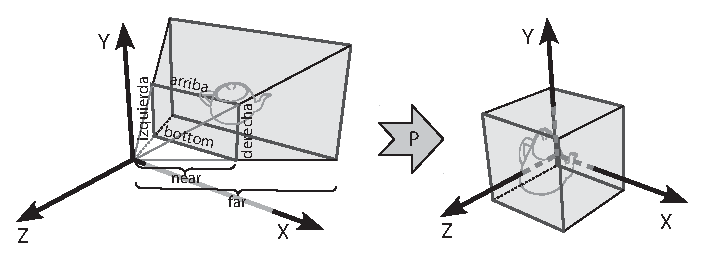
\includegraphics[width=\textwidth]{../figures/matriz_p.eps}
	\caption{La matriz P se encarga de transformar la pir�mide de visualizaci�n en un cubo unitario.}
	\label{figure_matriz_p}
\end{figure}

La composici�n de estas matrices producir� la matriz MVP. Esta es la expresi�n matem�tica usada para transformar cada punto: 
\begin{equation}\begin{split}v' & = \textbf{\textit{P}}\cdot \textbf{\textit{V}} \cdot \textbf{\textit{M}} \cdot v \\ & = \textbf{\textit{MVP}} \cdot v\end{split}\end{equation}    

Estos son los paso necesarios para la creaci�n de un \textit{frame}, pero puesto que le visualizador es interactivo, tendremos que repetir este proceso varias veces por segundo. 
%
% FIN DEL CAP�TULO
%

	%
% VISUALIZACIoN DE NUBES DE PUNTOS
%
\chapter{
	An�lisis y dise�o de un visualizador
	\label{nombre_referencia_al_capitulo_040}
}

En este cap�tulo se presentar� el resumen de dise�o que se sigui� en la creaci�n del visualizador de nubes de puntos.


%
% SECCION - T�cnicas de rasterizaci�n
%
\section[An�lisis de requisitos]{
	An�lisis de requisitos
	\label{s_analisis}
}

Ante la necesidad de un visualizador en el que poder probar los algoritmos que se iban a implementar, se pens� que ser�a buena idea el desarrollo de uno propio de manera que fuera simple, sencillo y f�cilmente modificable. 

El visualizador tendr�a que cumplir los siguiente requisitos:
\begin{itemize}
	\item Tener una gesti�n de \textit{shaders} de manera que fuera sencillo compilar y enviar a \textit{GPU} estos programas, adem�s de facilitar la incorporaci�n de nuevos en el proyecto.
	\item Carga de modelos desde ficheros en disco.
	\item Un sistema para almacenar las nubes de puntos y poderlas enviar a \textit{GPU} para su dibujado. 
	\item Una c�mara para moverse alrededor de los objetos cargados.
	\item Fuentes de luz para la iluminaci�n de la escena.
	\item Un \textit{framebuffer} donde almacenar los resultados.
\end{itemize}

\subsection{Casos de uso}

Se establecer�n los siguientes casos de uso (ver Figura \ref{figure_casos_de_uso}), siendo los m�s significativos:
\begin{itemize}
	\item La carga de modelos mediante ficheros externos (formatos .PLY o .PCD) destinados al almacenamiento de este tipo de datos.
	\item La opci�n para desactivar el color RGB de los puntos, de manera que sea mas claro evaluar si la reconstrucci�n de la superficie es correcta.
	\item La capacidad de moverse por el espacio tridimensional.
	\item Modificar el radio de los puntos manualmente o que el programa estipule un radio de manera automatica.
	\item Poder escoger entre los diferentes m�todos de rasterizaci�n o \textit{blending} implementados para variar la visualizaci�n de la nube.
	\item Cambiar el sistema de iluminaci�n.
\end{itemize}

\begin{figure}
	\centering
	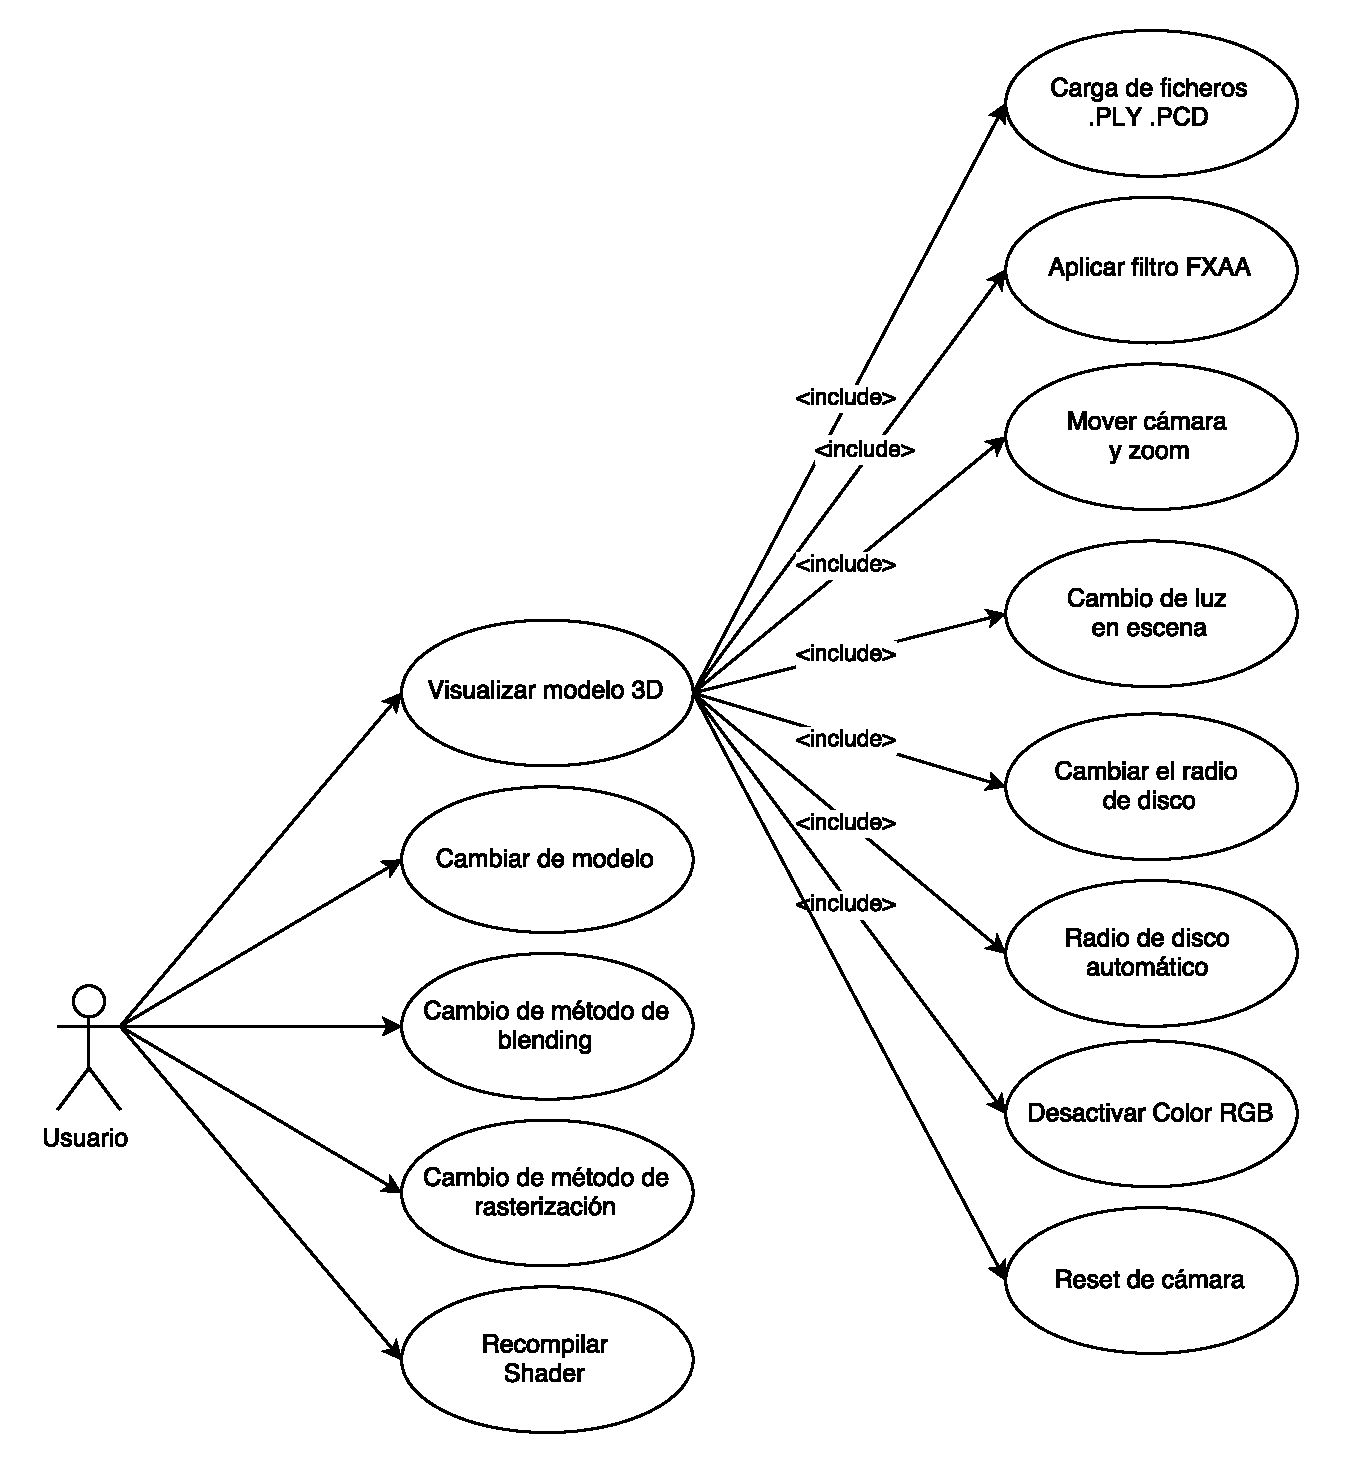
\includegraphics[width=\textwidth]{../figures/casosdeuso.pdf}
	\caption{Casos de uso de la aplicaci�n.}
	\label{figure_casos_de_uso}
\end{figure}


\section{Diagrama de clases}
Una vez definidos los requisitos, se pas� a dise�ar un esqueleto el cual se podr� ver en el siguiente diagrama de clases (ver Figura \ref{figure_diagram_class}):
\begin{figure}
	\centering
	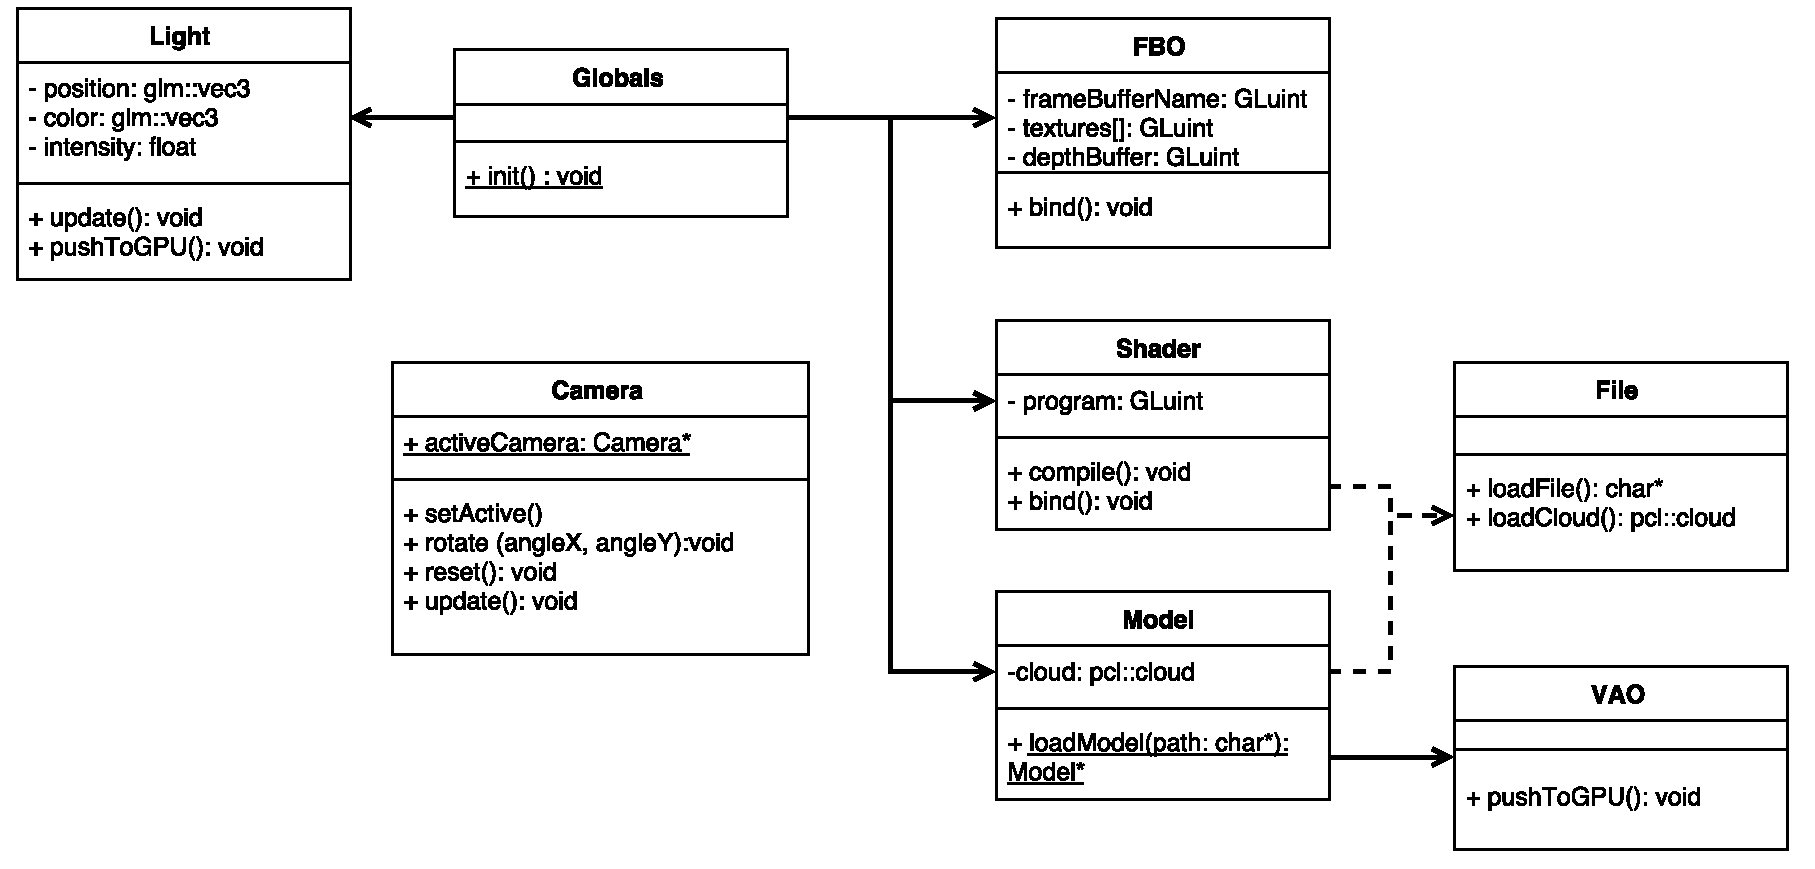
\includegraphics[width=\textwidth]{../figures/cubeUML.pdf}
	\caption{Diagrama de clases del visualizador de nubes de puntos.}
	\label{figure_diagram_class}
\end{figure}

La idea de tener un \textit{framebuffer} propio donde renderizar de manera separada (clase \textbf{FBO}), permiti� independizar el visualizador de la librer�a que fue usada para la creaci�n de ventanas en el Sistema Operativo\footnote{GLFW: http://www.glfw.org/}, de forma que en caso de necesitar cambiarla, esta escasa dependecia facilitar�a la tarea.

La clase \textbf{Shader}, vendr�a a dar la soluci�n al manejo de los \textit{vertex} y \textit{fragment shaders} en el visualizador, ofreciendo m�todos para compilar y enviar estos programas a \textit{GPU}.

La clase \textbf{Models} ser� la encargada de almacenar los modelos que se carguen. Estos almacenar�n los datos de la nube (posici�n, color, normal y radios).

El objetivo de la clase \textbf{VAO} ser� la de enviar la informaci�n de la nube de puntos al \textit{pipeline} y encargarse de reservar la memoria en la tarjeta gr�fica.

La clase \text{Camera} viene a ser la implementaci�n de todo lo explicado en la secci�n \ref{camera_model}, ofreciendo las matrices de transformaci�n pertinentes y que ser�n necesarias para el render. En este caso el funcionamiento de la c�mara es orbital, rotando alrededor de origen de coordenadas, pudiendo acercar o alejar la vista.

Se implementaron tres tipos diferentes de luz seg�n su comportamiento: una luz orbital que gira alrededor de un eje, una luz que se denomin� \textit{camera light} de forma que se pod�a fijar a una c�mara para que iluminara desde su posici�n y otra est�tica con motivo de tener luces de relleno inm�biles en la escena. Estas tres luces heredan de la superclase \textbf{Light}. 

La clase \textbf{Globals} nos permite almacenar variables donde almacenar las diferentes configuraciones que el usuario puede usar para ajustar la visualizaci�n a su gusto, adem�s de registrar otra informaci�n relevante as� como la posici�n del rat�n, dimensiones de la ventana, t�tulo ...

%
% FIN DEL CAP�TULO
%

	%
% VISUALIZACI�N DE NUBES DE PUNTOS
%
\chapter{
	Visualizaci�n de nubes de puntos en GPU
	\label{nombre_referencia_al_capitulo_050}
}

Este cap�tulo se presenta como un resumen a los diferentes m�todos de render basados en GPU. La secci�n \ref{s_rasterizacion} empieza mostrando los diferentes algoritmos que existen para la rasterizaci�n de splats. La secci�n \ref{s_blending} se centra en el blending de los diferentes splats, rasterizados en el paso previo, teniendo en cuenta la implicaci�n que toman diferentes aspectos como la iluminaci�n.


%
% SECCION - T�cnicas de rasterizaci�n
%
\section[T�cnicas de rasterizaci�n]{
	T�cnicas de rasterizaci�n
	\label{s_rasterizacion}
}

El primer paso en el render de nubes de puntos, es determinar seg�n la proyecci�n de los splats que p�xeles en el framebuffer ser�n cubiertos por ellos. Puesto que no existe soporte el las librer�as actuales para representar este tipo de primitivas, los splats tendr�n que ser representados por otras como puntos o tri�ngulos. De entre esas dos opciones, se  considera como m�s eficiente los puntos por delante de los tri�ngulos, ya que por cada splat unicamente hay que almacenar la posici�n de un v�rtice en lugar de tres. Finalmente para renderizar la nube, habr� que dibujar el \textit{VBO}, pas�ndole el tipo \textit{GL\_POINTS}
\\
\lstset{language=C, breaklines=true, basicstyle=\footnotesize}
\begin{lstlisting}[frame=single]
glDrawArrays(GL_POINTS, &splats[0], splats.size());
\end{lstlisting}

\subsection[Sized-Fixed Points] {Sized-Fixed Points \label{ss_sized}}

De una forma un poco primitiva y puesto que un punto a priori puede no tener un tama�o definido, a la hora de mostrar una representaci�n de la nube, se podr�a dibujar cada coordenada del conjunto de puntos, con un cuadrado de un tama�o definido. Para ello basta con activar en el programa.
\\
\lstset{language=C, breaklines=true, basicstyle=\footnotesize}
\begin{lstlisting}[frame=single]
glEnable(GL_PROGRAM_POINT_SIZE);
\end{lstlisting}

Mientras que en el \textit{vertex shader}, se define con \textit{gl\_PointSize} el tama�o en pixels que se pretente que ocupe el punto al ser rasterizado. Este cuadrado tendr� como centro las coordenadas del punto \textbf{p}.

\begin{figure}
	\centering
	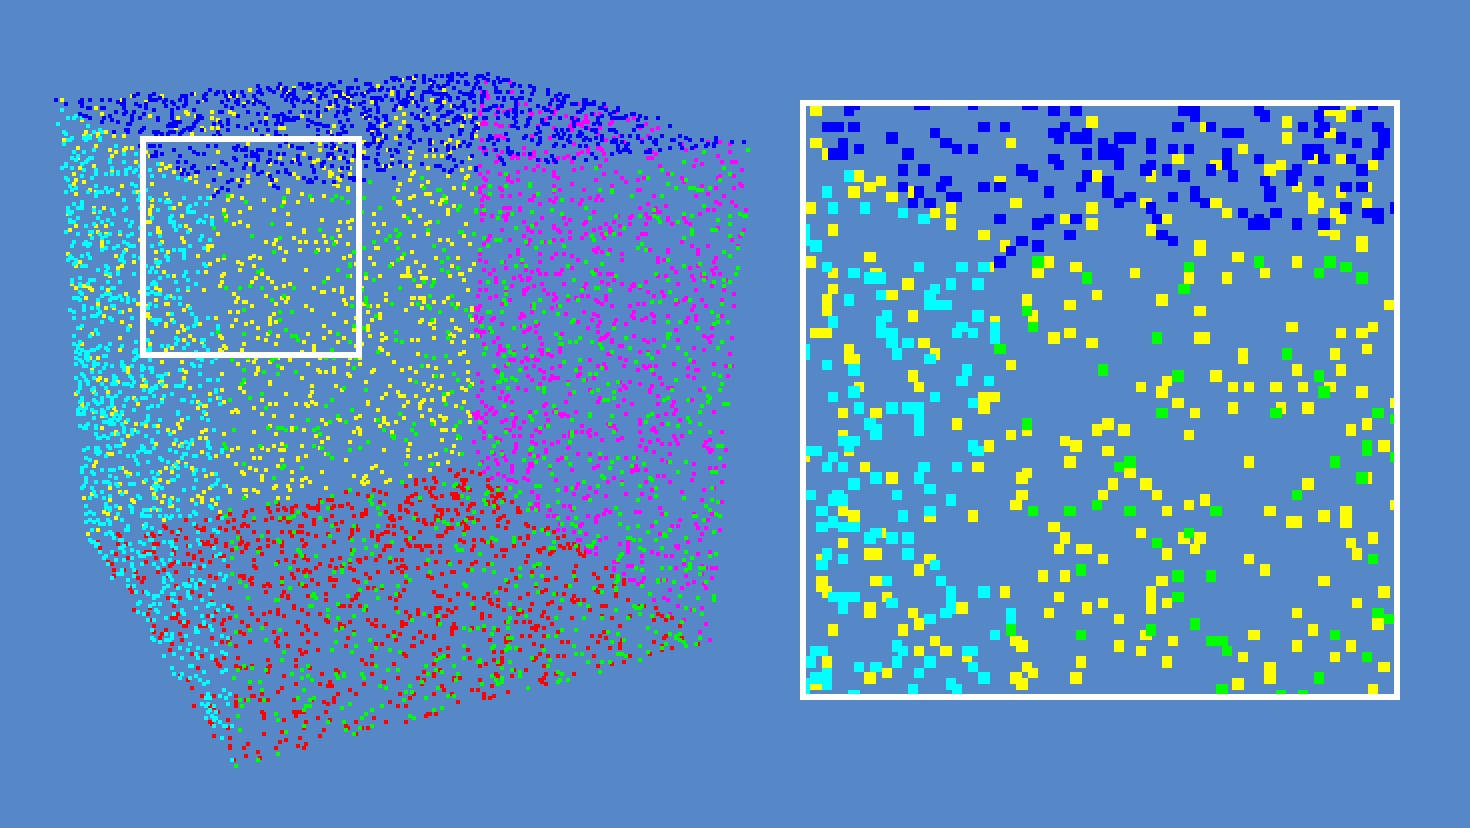
\includegraphics[width=\textwidth]{../figures/fixed-sized.png}
	\caption{Todos los puntos de la nube son renderizados con un cuadrado del mismo tama�o para toda la nube.}
\end{figure}

Como resultado, se obtiene una representaci�n en la que cada punto de la nube se renderizar� con el tama�o descrito.

Ver Ap�ndice Shaders \ref{sized-fixed}
\subsection[Image-aligned Squares] {Image-aligned Squares \label{ss_image-aligned_squares}}

En el anterior paso, el tama�o de la representaci�n que cada punto tomaba en el \textit{framebuffer} era de alguna forma independiente a la c�mara y al modelo.

De esta manera, si en lugar de entender el tama�o del punto como los pixeles que va a ocupar en la imagen final, se interpreta como una medida dentro del modelo, que podr�a ser el radio \textbf{r} del splat, al representarse, estos puntos tendr�an que ser coherentes con su proyecci�n.

As� que el tama�o en el \textit{screen-space} del punto OpenGL proyectado, tiene que ser ajustado en el \textit{vertex shader}. El tama�o \cite{perspcorrect} se aproxima haciendo el escorzo \textit{(perspective foreshort)} del radio $ r $ del splat usando el \textit{depth value} del centro \textbf{p} que ha de estar en coordenadas de la c�mara.

\begin{eqnarray}
gl\_PointSize = 2r \cdot \dfrac{n}{p_{z}} \cdot \dfrac{g}{t - b'}
\end{eqnarray}

Donde $ n $, $ t $ y $ b $ son los parametros \textit{near/top/bottom} del \textit{view frustum} y $ h $ denota la altura (en pixels) del \textit{viewport}. En esta f�rmula el t�rmino $ n/z $ corresponde a la proyecci�n en el plano \textit{near}, mientras que $ f/(t- b) $ escala el resultado desde el plano \textit{near} a coordenadas de la imagen.

Todos los pixels, generados de un punto, tienen el mismo \textit{depth value} lo que imposibilita hacer uso de las t�cnicas blending en zonas que visualmente se esten superponiendo. (ver secci�n \ref{s_blending})

Ver Ap�ndice Shaders \ref{image-aligned}

\subsection[Affinely Projected Point Sprites] {Affinely Projected Point Sprites \label{ss_affinely}}

Una mejor aproximaci�n para representar superfices afines a nubes de puntos, es con discos orientados seg�n un vector normal \textbf{n}, este m�todo fue presentado en \textit{Bosch and Kobbelt}~\cite{affinely} .

Para ello se tendr�a que ajustar el tama�o del punto en el \textit{vertex shader} de la misma forma que en el paso anterior \ref{ss_image-aligned_squares}. Pero a�adiendo a mayores en el \textit{fragment shader} alguna manera de determinar si este se corresponde con un fragmento de la proyecci�n de un disco orientado con centro en la posici�n \textbf{p}, de radio \textbf{r} y con la normal \textbf{n}. 

Para cada uno de los pixeles $ (x, y)  \in  [-r \;,\; r] $, se puede calcular un valor de desplazamiento en profundidad $ \delta z $ como una funci�n lineal dependiente del vector en coordenadas de la c�mara \textbf{n} = $(n_{x}, n_{y}, n_{z})^{T}$ :

\begin{equation}
	\delta z = - \dfrac{n_{x}}{n_{z}} \cdot x - \dfrac{n_{y}}{n_{z}} \cdot y
	\label{delta_z}
\end{equation}



Este desplazamiento es usado para calcular la distancia 3D desde el centro del punto \textbf{p}, de manera que el fragmento $ (x,y) $ corresponde al punto si $ ||(x,y,\delta z)|| \leq r $. Los que no cumplan esta condici�n pueden ser f�cilmente descartados usando el comando \textit{discard}. 

La variable vector \textit{gl\_PointCoord} del \textit{fragment shader} contiene las coordenadas bidimensionales que indican donde dentro de un punto OpenGL el fragmento est� situado, con valores desde el $ 0.0 $ al $ 1.0 $ estos han de desplazarse a un rango $ [-0.5 \;,\; 0.5] $ para usarse en el c�lculo de $ \delta z $.

Una posible implementaci�n de este algoritmo en \textit{GLSL} ser�a:
\\
\begin{lstlisting}[frame=single]
vec3 test;

test.x = gl_PointCoord.x - 0.5;
test.y = gl_PointCoord.y - 0.5;
test.z = -(normal.x/normal.z) * test.x - (normal.y/normal.z) * test.y;

if (length(test) > 0.5)
    discard;
\end{lstlisting}

Uno de los inconvenientes usando Image-aligned Squares \ref{ss_image-aligned_squares} era que el valor de profundidad era constante por splat. Pero $ \delta z $ puede ser usado tambi�n para corregir esto. Partiendo de un valor de profundidad en espacio de la c�mara $ z' = p_{z} + \delta z $ y el frustum el valor de profundidad del $ zbuffer(x,y) $ puede ser modificado

\begin{equation}
zbuffer(x,y) = \dfrac{1}{z'} \cdot \dfrac{fn}{f - n} + \dfrac{f}{f - n}
\label{z_buffer}
\end{equation} 

En comparaci�n con la propuesta de \textit{Image-aligned Squares}, este m�todo ofrece una mejor aproximaci�n, especialmente en los contornos del objeto. Sin embargo el valor de profundidad $ \delta z $ es solo una aproximaci�n, ya que se asume una proyecci�n paralela (\ref{delta_z}), causando errores que provocan que los discos se vuelvan demasiado finos cuando estos son mirados bajo �ngulos planos, lo que puede resultar en huecos en la imagen renderizada (ver Figura \ref{figure_affinely_holes}). 

\begin{figure}
	\centering
	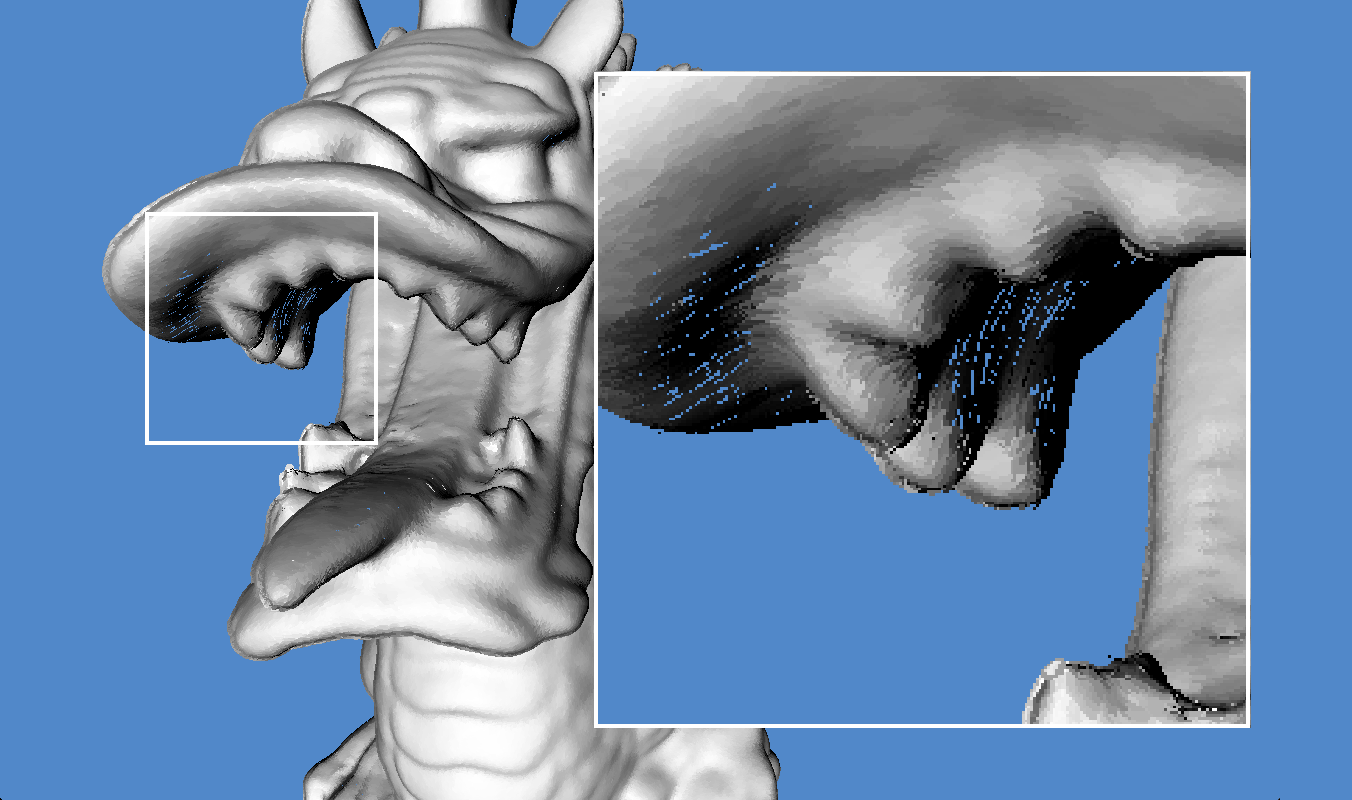
\includegraphics[width=\textwidth]{../figures/affinely-holes.png}
	\caption{Dragon, modelo de 845,281 puntos renderizado mediante Affinely Projected Point Sprites. Este m�todo causa huecos en �ngulos extremos.}
	\label{figure_affinely_holes}
\end{figure}

Ver Ap�ndice Shaders \ref{affinely}

\subsection[Perspective Correct Rasterization]{Perspective Correct Rasterization \label{ss_perspective_correct}}

El m�todo de \textit{Affinely Projected Point Sprites} (\ref{ss_affinely}) causaba errores debido a la proyecci�n paralela que en esta se asum�a. Puesto que la proyecci�n puede o no ser paralela, se tendr� que usar una aproximaci�n mas precisa. Esta t�cnica fue la propuesta por \textit{Bosch et al.}~\cite{perspective} . 

La idea principal de este procedimiento parte en determinar el punto 3D correspondiente al pixel 2D mediante un \textit{ray casting} local.

\begin{figure}
	\centering
	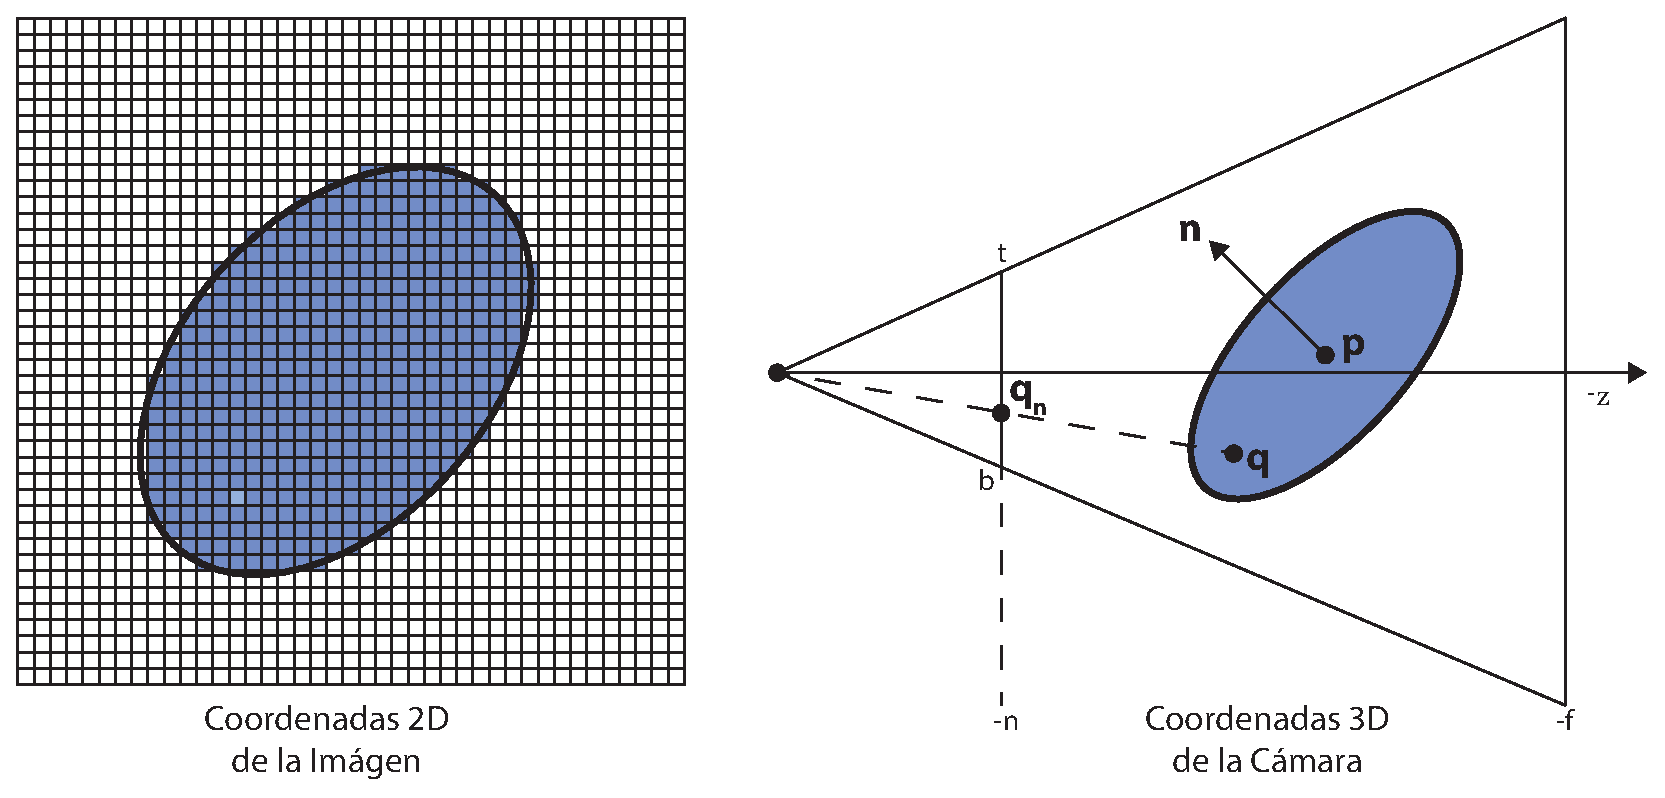
\includegraphics[width=\textwidth]{../figures/perspective-correct.eps}
	\caption{Proyecci�n y Ray Casting.}
	\label{figure_perspective_correct}
\end{figure}

Fij�ndose en el \textit{pipeline} de transformaciones de OpenGL el primer paso para calcular \textbf{q} es invertir la transformaci�n \textit{window-to-viewport}, de esta manera se mapear� el pixel \textit{(x,y)} a un punto 3D {$ \mathbf{q_{n}} $} en el plano \textit{near}. 

\begin{eqnarray}
q_{n} = 
\begin{pmatrix} 
	x \cdot \dfrac{r-l}{w} - \dfrac{r-l}{2} \\ 
	y \cdot \dfrac{t-b}{h} - \dfrac{t-b}{2} \\ 
	-n 
\end{pmatrix}
\end{eqnarray} 

Donde \textit{x/y} son las coordenadas relativas a la ventana \textit{gl\_FragCoord.xy}, \textit{b/t/l/r} son los par�metros \textit{bottom/top/left/right} del \textit{viewing frustum}, y \textit{w/h} denotan la \textit{altura/anchura} del \textit{viewport} (ver Figura \ref{figure_perspective_correct}).

Se proyectar� un rayo desde el origen (el ojo de la c�mara) a traves de {$ \mathbf{q_{n}} $} y la intersecci�n con el plano del \textit{splat} \textbf{p} dar� como resultado el punto \textbf{q}. En caso de que $ q_{n} \cdot n = 0 $ se determinar� que el el �ngulo el por lo que se podr� descartar el \textit{splat}. 

\begin{equation}
q = q_{n} * \dfrac{p \cdot n}{q_{n} \cdot n}
\label{q}
\end{equation} 

Finalmente el pixel ser� descartado si $ \| q - p \| > r $. Por otro lado el valor de profundidad del \textit{z-buffer} puede ser ajustado insertando $ q_{z} $ como valor de $ z' $ en la ecuaci�n (\ref{z_buffer}). 

\begin{figure}
	\centering
	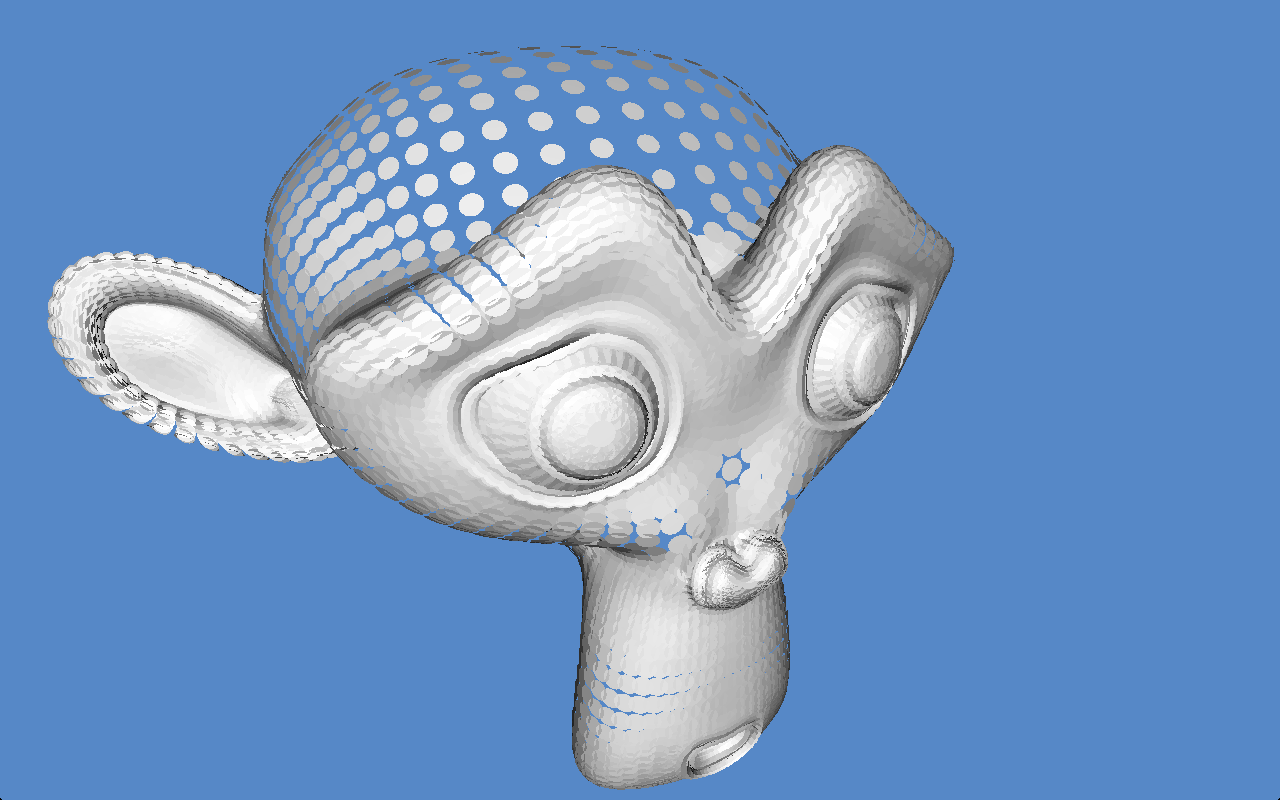
\includegraphics[width=\textwidth]{../figures/perspective-correct-flat.png}
	\caption{Suzanne, modelo de 7,958 puntos renderizado mediante Perspective Correct Rasterization.}
	\label{figure_perspective_correct_render}
\end{figure}

Ver Ap�ndice Shaders \ref{perspective}

%
% SECCION - T�cnicas de Blending
%
\section[T�cnicas de Blending]{
	T�cnicas de Blending
	\label{s_blending}
}

Luego de determinar los pixels que son cubiertos por la proyecci�n de los \textit{splats} en el anterior paso de rasterizaci�n, el siguiente implica iluminaci�n y en general el acabado est�tico de la superficie \textit{shading}.

% Subsecci�n
\subsection[Flat Shading] {Flat Shading \label{ss_flat}}

Puesto que cada punto tiene asociado un vector normal \textbf{n}, para unas ciertas propiedades de material y reflectancia una iluminaci�n local puede ser evaluada por \textit{splat}. Como resultado se obtendr� una constante de color $ \mathbf{c_{i}} $ para cada splat, similar al \textit{flat shading} en modelos poligonales. Ya que los puntos tienden a intersecar unos con otros, las representaciones mediante \textit{flat shading} conllevan a discontinuidades en el color.

\subsection[Gouraud Shading] {Gouraud Shading \label{ss_gouraud}}

\begin{figure}
	\centering
	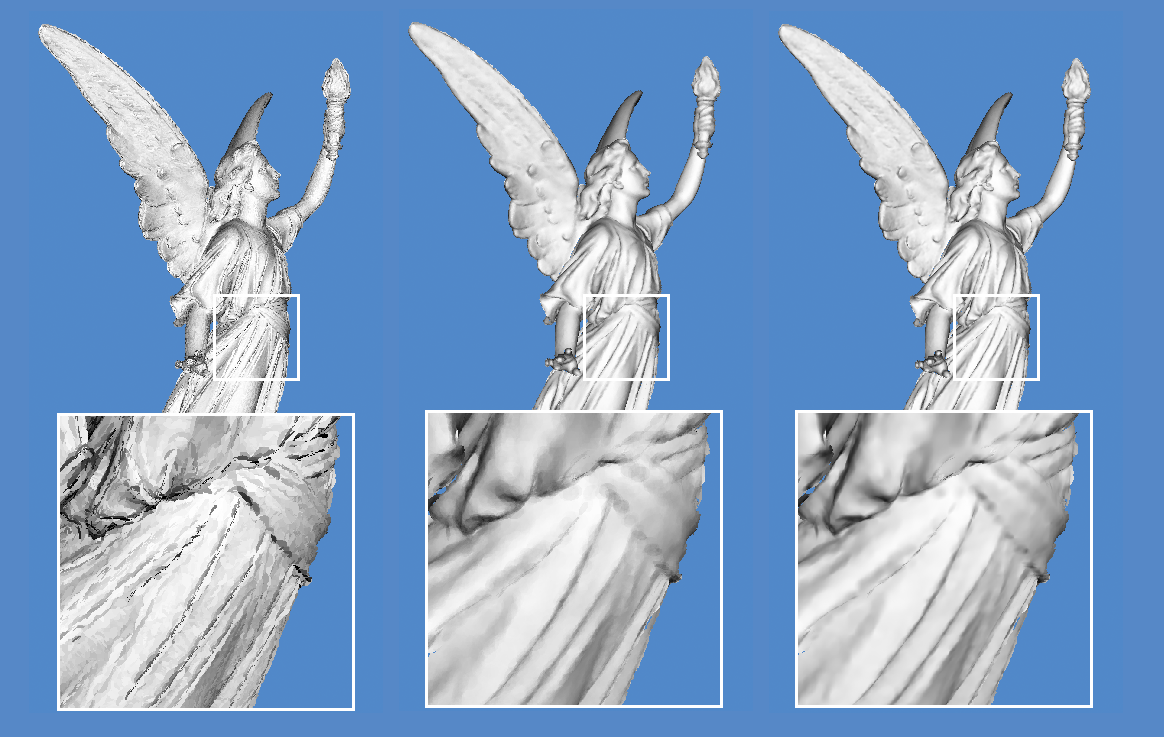
\includegraphics[width=\textwidth]{../figures/comparacion_blending.png}
	\caption{Lucy, modelo de 397,664 puntos. Renderizado mediante \textit{Flat Shading} (\textbf{izquierda}), \textit{Gouraud Shading} (\textbf{centro}), y \textit{Phong Shading} (\textbf{derecha}).}
	\label{figure_blending_comparative}
\end{figure}

Para conseguir un render mas fino, las discontinuidades en el color provocadas por el \textit{shading} pueden ser emborronadas mediante \textit{blending} de los valores de color $ \mathbf{c_{i}} $ de los puntos que se est�n superponiendo. Puesto que los c�lculos de iluminaci�n todav�a son computados por \textit{splat}, este tipo de \textit{blending} del color, conceptualmente corresponde al \textit{Gouraud shading} de modelos poligonales.

Para implementar este tipo de \textit{blending} cada punto de la nube ir� asociado con una funci�n, de modo que para cada \textit{splat} sus fragmentos ir�n teniendo menor peso $ \mathbf{r}$ cuanto mas alejados de su centro est�n, teniendo as� menor impacto en la mezcla final de color $ \mathbf{c(x, y)} $. De manera que en la reconstrucci�n final del \textit{framebuffer}, el color de la posici�n $ (x,y) $ vendr� dado por el peso promedio de todos los fragmentos $ \mathbf{i} $ que intenten cubrirlo.

\begin{equation}
\mathbf{c}(x,y) = \dfrac{\sum_{i}^{} r_{i}(x,y) \; c_{i}}{\sum_{i}^{} r_{i}(x,y)}
\end{equation}

Esta media puede ser implementada en OpenGL usando 2 pases de render. Primero, el \textit{alpha-blending} es configurado con funciones separadas de \textit{blend} para las componentes RGB y alpha \textit{EXT\_blend\_func\_separate} con
\\
\begin{lstlisting}[frame=single]
glEnable(GL_BLEND);
glBlendFuncSeparateEXT(GL_SRC_ALPHA, GL_ONE, GL_ONE, GL_ONE);
\end{lstlisting}

As� los \textit{splats} ir�n acumulando los valores de color y peso en
las componentes RGB y alpha del \textit{framebuffer} como $ (
\sum_{i}^{} r_{i} c_{i} \;,\; \sum_{i}^{} r_{i} ) $. Finalmente tendr�
que normalizarse la componente \textit{RGB} de cada pixel,
dividiendose por su componente \textit{alpha}. Esto puede ser
conseguido enviando el resultado del anterior pase a un siguiente como
una textura, renderizando un rect�ngulo de tama�o de la ventana y
mapeando esta textura en el. Este truco conocido como
\textit{render-to-texture}, envia de nuevo cada pixel a trav�s del
\textit{pipeline} de OpenGL, de modo que un simple \textit{fragment
  shader} puede realizar esta normalizaci�n, como la propuesta en \textit{Botsch and Kobbelt}~\cite{affinely} y en \textit{Guennebaud and Paulin}~\cite{Efficient_screen}. Esta acumulaci�n debe de ser realizada usando \textit{buffers} con precisi�n de punto flotante de 16 bits, con motivo de evitar saturaciones o artefactos.

Para restringir el \textit{blend} �nicamente a la superposici�n de los \textit{splats} vecinos de la misma superficie. Es necesario un tercer pase, denominado de visibilidad. Para cada \textit{frame}, el pase de visibilidad primero renderiza la nube unicamente en el \textit{depth buffer}. Luego en el pase de \textit{blending} se renderiza la nube de nuevo, pero esta vez calculando iluminaci�n y acumulando el valor resultante de color usando \textit{additive alpha-blending} como lo descrito anteriormente. En este pase no se debe de actualizar el \textit{z-buffer} calculado en el pase de visibilidad, pero s� se a�ade un desplazamiento $\epsilon$ a todos los valores de profundidad~\cite{surface_splatting}, lo que provocar� que todos los fragmentos dentro de una distancia $\epsilon$ sean mezclados. El pase final de normalizaci�n realiza la necesaria divisi�n por el componente \textit{alpha} como se describi� anteriormente. El resultado de los tres pases de render es representado en la Figura \ref{figure_gouraud_pipeline}.

\begin{figure}
	\centering
	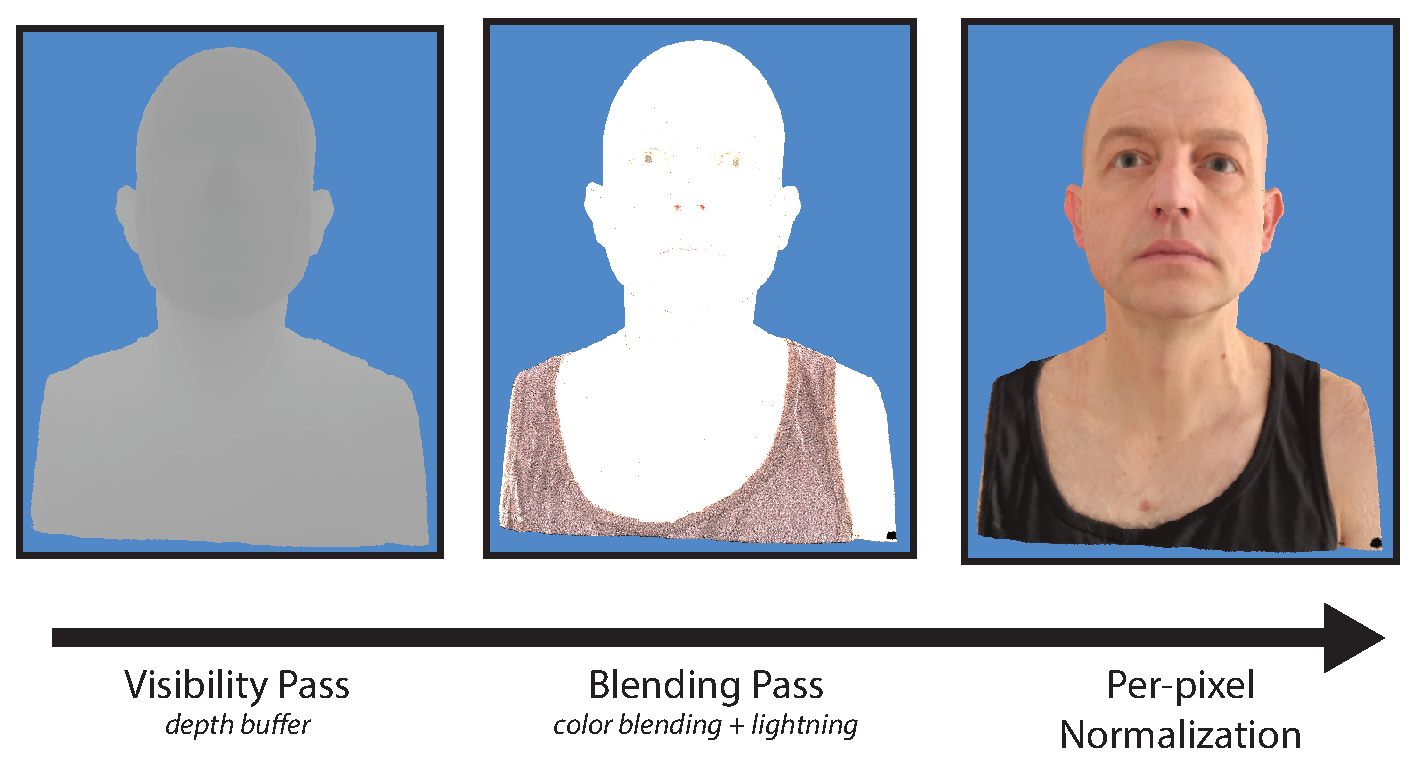
\includegraphics[width=\textwidth]{../figures/gouraud-pipeline.eps}
	\caption{Los tres pases, \textit{visibility}, \textit{blending}, y \textit{normalization}.}
	\label{figure_gouraud_pipeline}
\end{figure}

El \textit{pseudocode} ser�a el siguiente
\begin{lstlisting}[frame=single]
// visibility pass
glDepthMask(GL_TRUE);
glDisable(GL_BLEND);
bind_visibility_shaders();
glDrawArrays(GL_POINTS, &cloud[0], cloud.size());

// blending pass
glDepthMask(GL_FALSE);
glEnable(GL_BLEND);
bind_blending_shaders();
glDrawArrays(GL_POINTS, &cloud[0], cloud.size());

// normalization pass
glCopyTexSubImage2D(GL_TEXTURE_RECTANGLE_ARB, 0, 0, 0, 0, 0, w, h);
bind_normalization_shaders();
draw_rectangle();
\end{lstlisting}

Ver Ap�ndice Shaders \ref{gouraud}

\subsection[Phong Shading] {Phong Shading \label{ss_phong}}

Cuando se comparan los resultado de las diferentes t�cnicas en la figura \ref{figure_blending_comparative}, \textit{Gouraud} realmente elimina las indeseadas discontinuidades de color provocadas en el \textit{Flat Shading}, pero tambi�n a�ade cierto emborrone a la imagen notablemente. Para renderizado de pol�gonos es bien conocido que \textit{Phong} es superior que \textit{Gouraud Shading}. En lugar de calcular la iluminaci�n por cada v�rtice y linealmente interpolar el color resultante dentro de los tri�ngulos, \textit{Phong} interpola las normales en los v�rtices, seguido de una iluminaci�n por p�xel basada en la resultante funci�n definida a trozos.

Pero ya que en el caso de las nubes de puntos falta la relaci�n de conectividad, no es posible la interpolaci�n de las normales de los puntos vecinales, de modo que el campo de normales deber� ser construido de otra forma.

El m�todo de \textit{Phong} de \textit{Botsch et al.}~\cite{perspective} asigna expl�citamente un campo de normales lineal $ \mathbf{n_{i}}(x,y) $ para cada \textit{splat} en lugar de mantener su normal asociada constante. Durante la rasterizaci�n, la normal es evaluada para cada pixel bas�ndose en sus parametros locales \textit{(x, y)}, y el vector resultante $ \mathbf{n_{i}}(x,y)$ es usado para computar la iluminaci�n. Ya que los valores de color resultantes siguen teniendo problemas de discontinuidad, estos son acumulados y mezclados usando el mismo sistema de 3 pases de \textit{Gouraud}. La unico que queda por conocer entonces es saber como computar el campo de normales lineal $ \mathbf{n_{i}}(x,y) $. Cada normal ser� representada por un punto (x,y) en el plano tangente con distancia 1, similar a las coordenadas homog�neas (Figura \ref{figure_phong_normal}). 

\begin{figure}
	\centering
	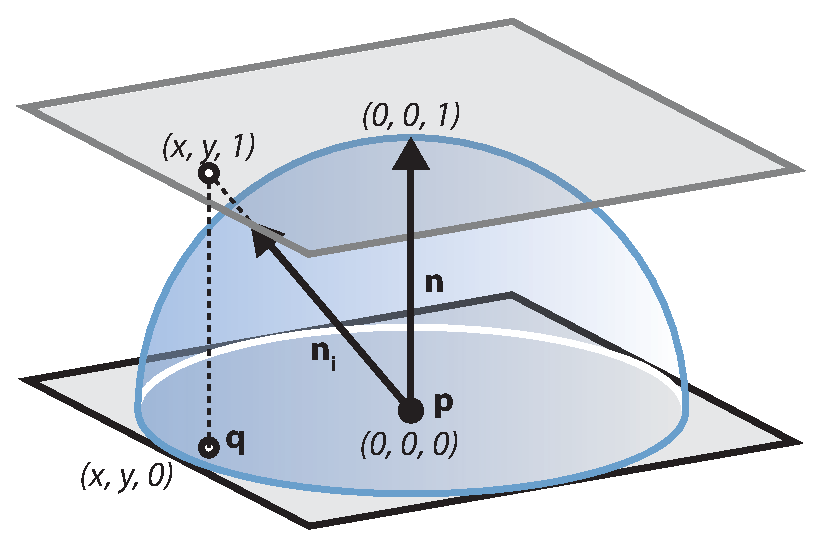
\includegraphics[width=7 cm]{../figures/phong.eps}
	\caption{Los vectores $ n_{i} $ son representados como puntos homog�neos \textit{(x,y,1)} en un plano desplazado tangente.}
	\label{figure_phong_normal}
\end{figure}

\begin{equation}
n_{i} = \dfrac{(q + n) - p}{\|(q + n) - p\|}
\end{equation}

Donde \textbf{q} es el punto 3D del \textit{splat} calculado al igual que en el m�todo de \textit{Perspective Correct Rasterization} (Ecuaci�n \ref{q}), \textbf{n} es la normal del \textit{splat} y \textbf{p} es el centro de este en coordenadas de la c�mara.

Ver Ap�ndice Shaders \ref{phong}

\subsection[Deferred Shading] {Deferred Shading \label{ss_deferred}}

B�sicamente existen dos formas para generar interpolaciones suavizadas de vectores de normales. La primera es \textit{Phong} que como se coment� en el anterior apartado, utiliza funciones para calcular el campo de normales de un \textit{splat}. Una segunda opci�n pasar�a por la denominada como \textit{deferred} en la que en lugar de mezclar en un misma fase color y normales, estas se calculan de forma separada.

\begin{figure}
	\centering
	\includegraphics[width=\textwidth]{../figures/deferred_pipeline.eps}
	\caption{El renderizado mediante \textit{Deferred Shading} acumula atributos como color y normales, seguido por una normalizaci�n y un shading pass.}
	\label{figure_deferred_pipeline}
\end{figure}

Recientes generaciones de \textit{GPU} contienen todo lo necesario para implementear esta aproximaci�n, que gracias al denominado \textit{multiple render targets} (\textit{ARB\_DRAW\_BUFFERS}) permite que en un simple pase de \textit{render} se puedan sacar diferentes resultados a diferentes \textit{buffers}, estas caracter�sticas habilitan la opci�n para poder implementar una iluminaci�n por pixel (\textit{deferred}) en este contexto, como se demostr� en \textit{Botsch et al.}~\cite{deferred}

Primeramente en el pase de visibilidad (ver Figura \ref{figure_deferred_pipeline}, izquierda), se har� una modificaci�n para poder sacar en un target a parte la posici�n 3D del fragmento, \textbf{q} (ver. Ecuaci�n \ref{q}) ya que ser� necesario para el pase final. Luego, en el pase de acumulaci�n y blend (ver Figura \ref{figure_deferred_pipeline}, centro) se usar�n 2 targets adicionales para sacar la salida referente al color y de las normales de manera separada, usando el mismo proceso de acumulaci�n que en \textit{Gouraud}. Finalmente estos 3 \textit{buffers} ser�n enviados de nuevo al \textit{pipeline} de OpenGL, usando el m�todo de \textit{render to texture} comentado previamente, con motivo de su normalizaci�n.

Este �ltimo pase (ver Figura \ref{figure_deferred_pipeline}, derecha), corresponde a la fase de normalizaci�n de \textit{Gouraud} pero en el que a mayores se van a realizar los c�lculos pertinentes para la iluminaci�n. Por cada pixel, una media de la normal y el color pueden ser obtenidos, que junto a la posici�n obtenida en la primera fase de visualizaci�n puede ser f�cilmente calcular el color final iluminado.

Es importante darse de cuenta de que en este m�todo los c�lculos derivados de la iluminaci�n son computados una �nica vez por pixel, en contraste con las aproximaciones que no son \textit{deferred} que incorporan este proceso en el momento de la rasterizaci�n, consiguiendo el color final del pixel a partir de la mezcla de muchos pixels de diferentes \textit{splats} iluminados previamente. Dependiendo del n�mero de \textit{splats} superpuestos, esto puede llegar a multiplicar el numero de c�lculos derivados de la iluminaci�n.

Adem�s a esto, \textit{deferred shading} a�ade tambi�n una clara separaci�n entre la fase de rasteriaci�n y de iluminaci�n.

Ver Ap�ndice Shaders \ref{deferred}

%
% FIN DEL CAP�TULO
%

	%
% RESULTADOS Y RENDIMIENTO
%
\chapter[Resultados y rendimiento]{
	Resultados y rendimiento
	\label{nombre_referencia_al_capitulo_060}
}

En este cap�tulo se pasar�n a analizar los resultados obtenidos de la ejecuci�n de los diferentes algoritmos de visualizaci�n. Se empezar� por los 4 m�todos de rasterizaci�n: \textit{Sized-Fixed} (ver. \ref{ss_sized}), \textit{Image-aligned Squares} (ver. \ref{ss_image-aligned_squares}), \textit{Affinely Projected} (ver. \ref{ss_affinely}) y \textit{Perspective Correct} (ver.\ref{ss_perspective_correct}). Seguidamente se comentar�n los resultados obtenidos de la comparaci�n de los 4 sistemas de \textit{blending}: \textit{Flat} (ver. \ref{ss_flat}), \textit{Gouraud} (ver. \ref{ss_gouraud}), \textit{Phong} (ver. \ref{ss_phong}), \textit{Deferred} (ver. \ref{ss_deferred}) y la estabilidad de estos algoritmos en temas de iluminaci�n.

\section[Preparaci�n de la prueba] {Preparaci�n de la prueba}
Se dispuso del mismo equipo (ver Tabla. \ref{computer_specifications}) para la obtenci�n de los datos necesarios con motivo de analizar el rendimiento que presentan los diferentes algoritmos mencionados anteriormente. As� mismo se dispuso de un conjunto de 6 modelos que fueron sampleados a diferentes densidades (ver Tabla. \ref{models_specifications}).

\begin{table}
	\centering
	\begin{tabular}{l r}
		\hline
		\textbf{Equipo de Test} \\
		\hline \hline
		CPU: & Intel Core i7-4930K \\
		Tarjeta Gr�fica: & NVIDIA GTX 780Ti \\
		RAM: & 16 GB DDR3 a 2133 MHz \\
		HDD: & WD Caviar Black HDD \\
		SO: & Windows 7 \\
		\hline
	\end{tabular}
	\caption {Resumen de las caracter�sticas del equipo de Test.}
	\label{computer_specifications}
\end{table}

\begin{table}
	\centering
	\begin{tabular}{l r}
		\hline
		\textbf{Modelo} & \textbf{N�mero de puntos}\\
		\hline \hline
		Suzanne & 473672\\
		Head (Ten24) & 1223693 \\
		Dorna & 2585907 \\
		Dragon & 8628877 \\
		Happy Budha & 26519484 \\
		Lucy & 43982232 \\
		\hline
	\end{tabular}
	\caption {Los modelos utilizados en el test.}
	\label{models_specifications}
\end{table}

El par�metro que se estudiar� ser� el tiempo (en segundos) que se tarda en renderizar un \textit{frame}. El visualizador consta con un modo \textit{DEBUG} en el que autom�ticamente escribe en un \textit{log} los datos resultantes de la sesi�n. Este fichero tendr� el siguiente formato:

\begin{lstlisting}[frame=single, basicstyle=\tiny]
CUBE | Sized-Fixed Points | Flat Shading | RGB | 6000 Points | 0 Lights | 640x480
0.0152009
0.016681
0.016721
0.016681
CUBE | Sized-Fixed Points | Flat Shading | RGB | 6000 Points | 0 Lights | 1920x1058
0.0144408
0.016641
0.016681
0.016641
0.016641
0.016681
\end{lstlisting}

Este consta de una linea cabecera en la que se resume el escenario actual, continuando de los tiempos medios resultantes de los �ltimos 25 \textit{frames}.

Con motivo de facilitar el an�lisis de los datos obtenidos, se cre� una herramienta con el prop�sito de automatizar el an�lisis de este fichero \textit{log} y generar autom�ticamente las gr�ficas necesarias para su comprensi�n. \\

\begin{lstlisting}[frame=single, basicstyle=\tiny]
CUBE GRAPH GENERATOR

USAGE: cubeGraphGen.py [options] logFile

OPTIONS:
-h        Display available options
--help    Display available options
-v        Run in verbose mode
May the Force be with you :)
\end{lstlisting}

\section[An�lisis de los m�todos de rasterizaci�n] {An�lisis de los m�todos de rasterizaci�n}

Se renderizaron los 6 modelos (ver. Tabla \ref{models_specifications}) mediante los 4 m�todos de rasterizaci�n, sin filtro de antialiasing, iluminaci�n o \textit{blending}. El resultado de este an�lisis lo podemos ver en la siguiente gr�fica (ver Figura \ref{figure_rasterization_graph}).

Se encontr� que en cuanto aument� notablemente el n�mero de puntos a dibujar, el rendimiento del supuestamente m�s ligero de todos los algoritmos \textit{Sized-Fixed} cay� estrepitosamente, debido a que al tener el tama�o de punto definido de forma constante este estar�a generando m�s fragmentos en comparaci�n con los otros 3 que corrigen su tama�o en funci�n de la profundidad y de la distancia con los n-vecinales.

Adem�s en comparaci�n con los algoritmos que utilizan las normales para la representaci�n, en el algoritmo \textit{Affinely Projected} al no poder hacer \textit{backface culling} aumentan el n�mero de puntos a mostrar aumentando el tiempo de \textit{render}.

\begin{figure}
	\centering
	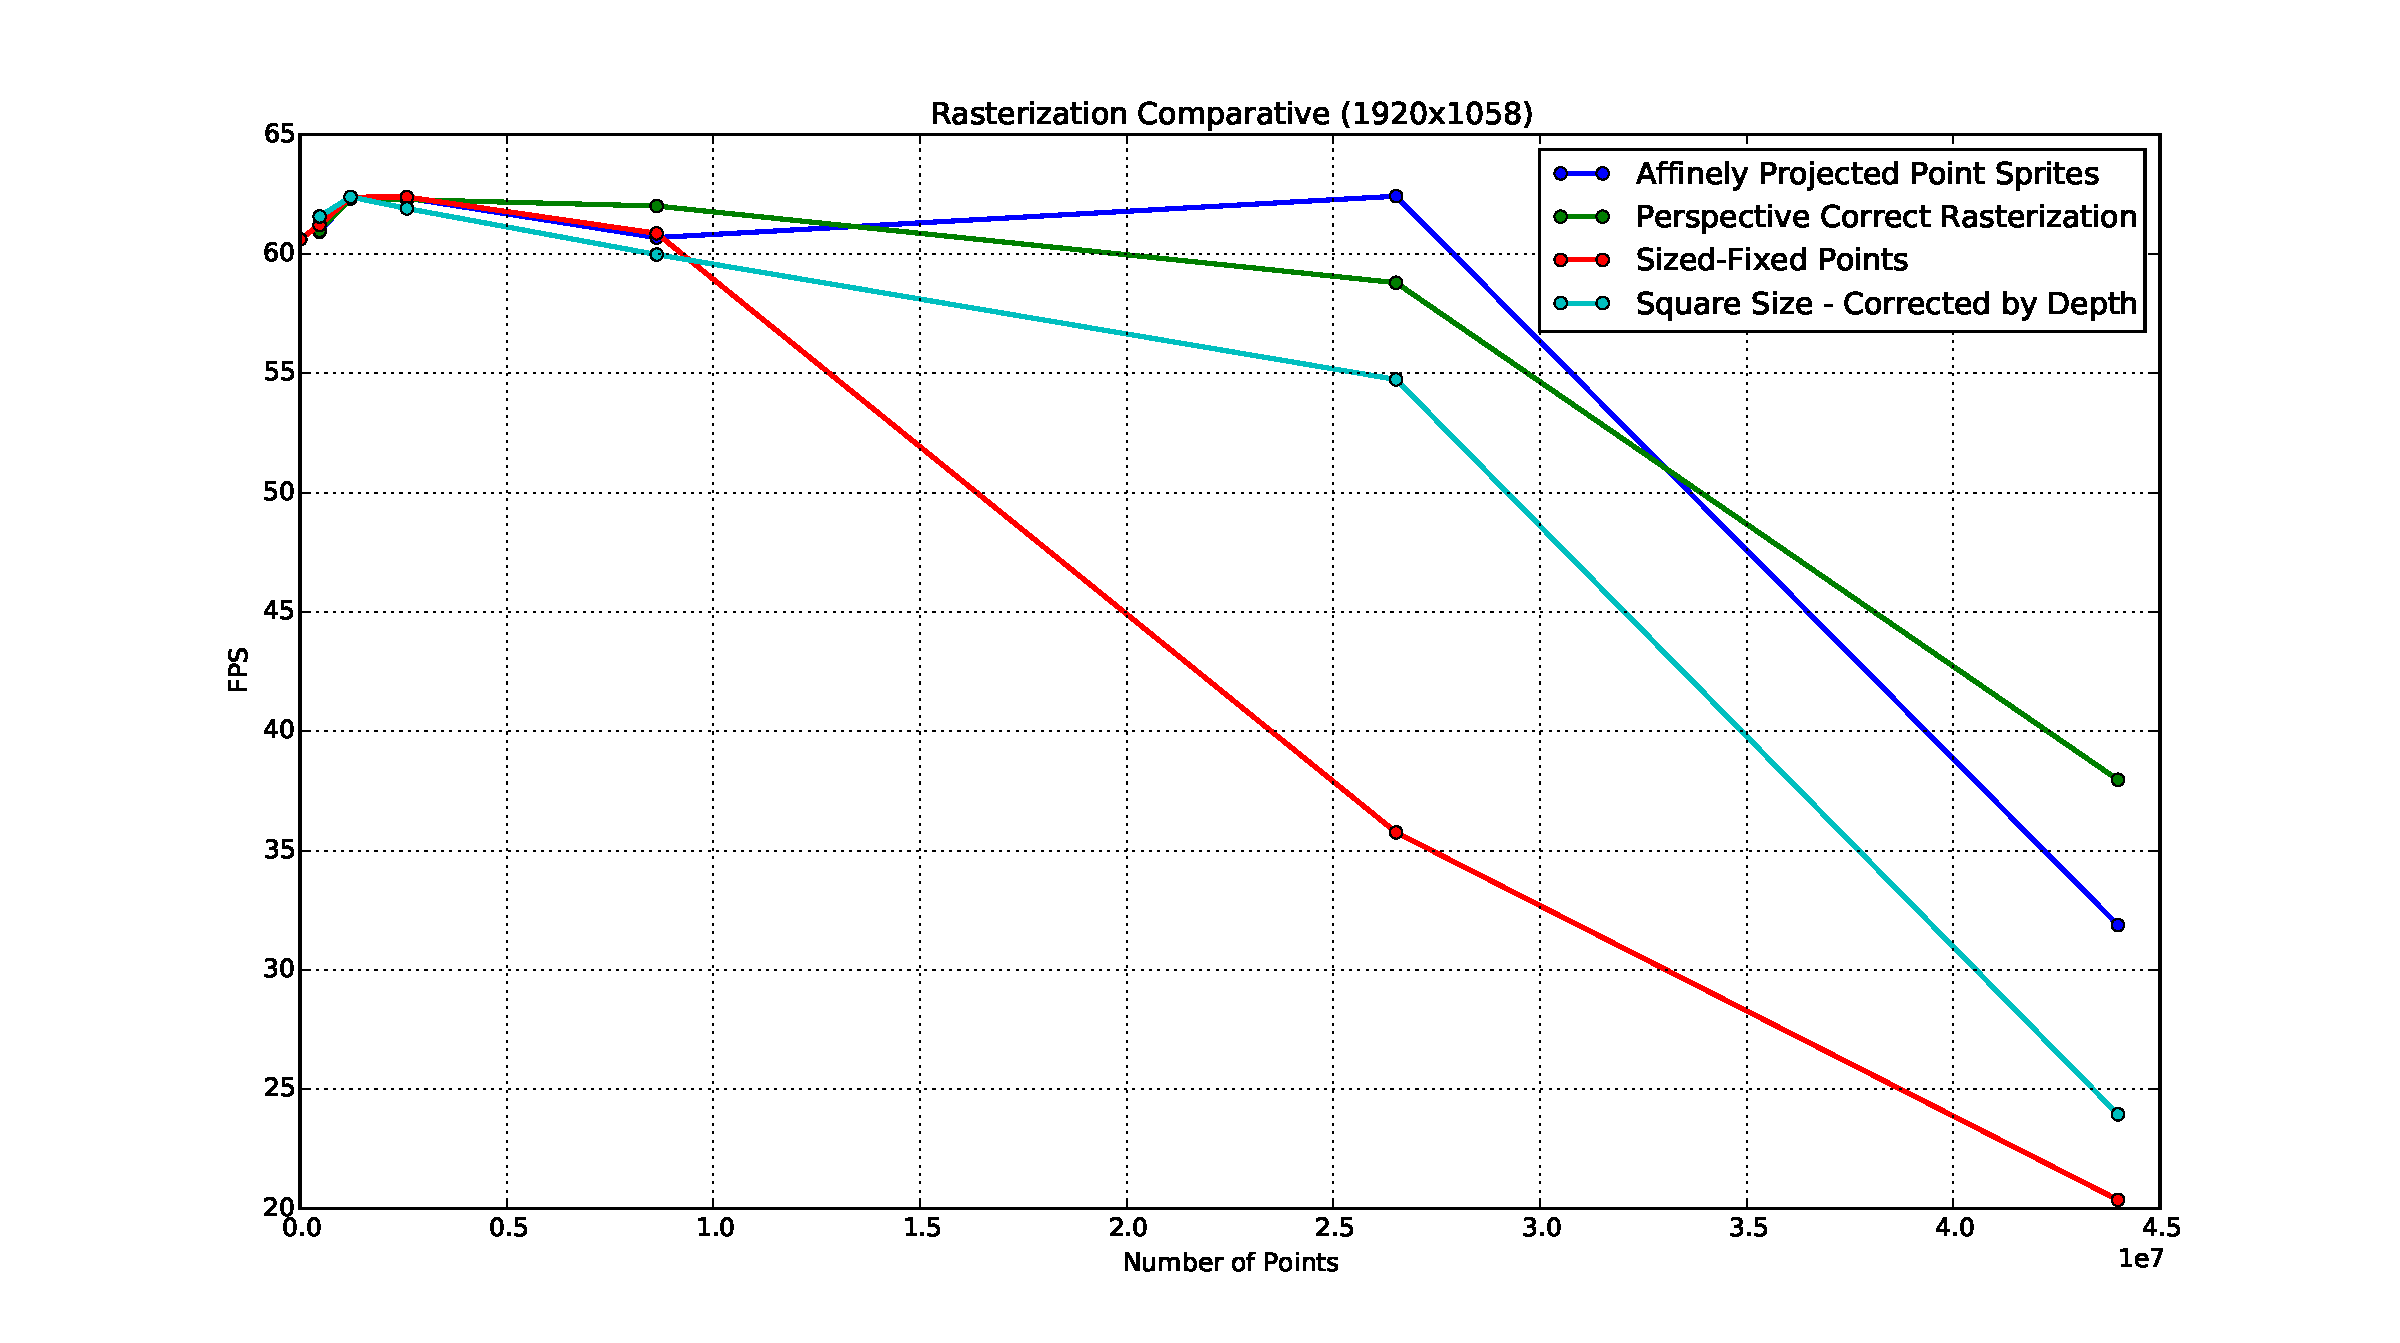
\includegraphics[width=\textwidth]{../figures/rasterization_graph.pdf}
	\caption{Gr�fica comparativa de los 4 sistemas de rasterizaci�n.}
	\label{figure_rasterization_graph}
\end{figure}

Con respecto al aspecto visual (ver Figura \ref{figure_rasterization_comparative}), encontramos que:

\begin{itemize}
	\item  El algoritmo \textit{Sized-Fixed} crea agujeros de forma incontrolable, ya que dependiendo de la distancia a la que en la que se encuentren los puntos, puede dar sensaci�n de superficie cerrada o de nube dispersa.
	\item El algoritmo de \textit{Square Aligned} consigue cerrar la superficie pero deforma los contornos notablemente.
	\item El algoritmo \textit{Affinely Projected} da una sensaci�n buena, pero da lugar a fallos con discos con algulos perpendiculares al plano \textit{near} de la c�mara. (ver Figura \ref{figure_affinely_holes})
	\item El m�todo de \textit{Perspective Correct} consigue mantener el contorno, ademas de evitar los agujeros de la anterior aproximaci�n.
\end{itemize}

\begin{figure}
	\centering
	\includegraphics[width=\textwidth]{../figures/comparacion_raster.eps}
	\caption{Comparativa de los resultados de render. \textit{Sized-fixed} (\textbf{izquierda}), \textit{Square-aligned} (\textbf{centro izquierda}), \textit{Affinely} (\textbf{centro derecha}) y \textit{Perspective Correct} (\textbf{derecha}).}
	\label{figure_rasterization_comparative}
\end{figure}

\section[An�lisis de los m�todos de blending empleados] {An�lisis de los m�todos de blend empleados}

Se renderizaron los seis modelos (ver. Tabla \ref{models_specifications}) mediante los cuatro m�todos de \textit{blending}, sin filtro de \textit{antialiasing} ni iluminaci�n. El resultado de este an�lisis lo podemos ver en la siguiente gr�fica (ver Figura \ref{figure_blending_graph}).

Se concluy� que como se esperaba, el m�todo de renderizado en un pase (sin \textit{blending}) alcanza mejores tiempos de \textit{render} en comparaci�n con los otros tres algoritmos que constan de tres pases para su dibujado. Teniendo estos tres un resultado bastante similar y peor con respecto al \textit{Flat Shading}.

Comparando al acabado visual de los algoritmos (ver Figura \ref{figure_blending_comparative}) encontramos que:
\begin{itemize}
	\item \textit{Flat Shading} no elimina las discontinuidades consecuencia de la intersecci�n y solape de los discos.
	\item \textit{Gouraud Shading} elimina las discontinuidades a�adiendo cierto desenfoque en su acabado.
	\item \textit{Phong} como \textit{Deferred Shading} eliminan las discontinuidades, a�adiendo mas definici�n que el anterior, puesto que se hace una interpolaci�n de las normales. Siendo el resultado de estos dos m�todos es pr�cticamente similar.
\end{itemize}

\begin{figure}
	\centering
	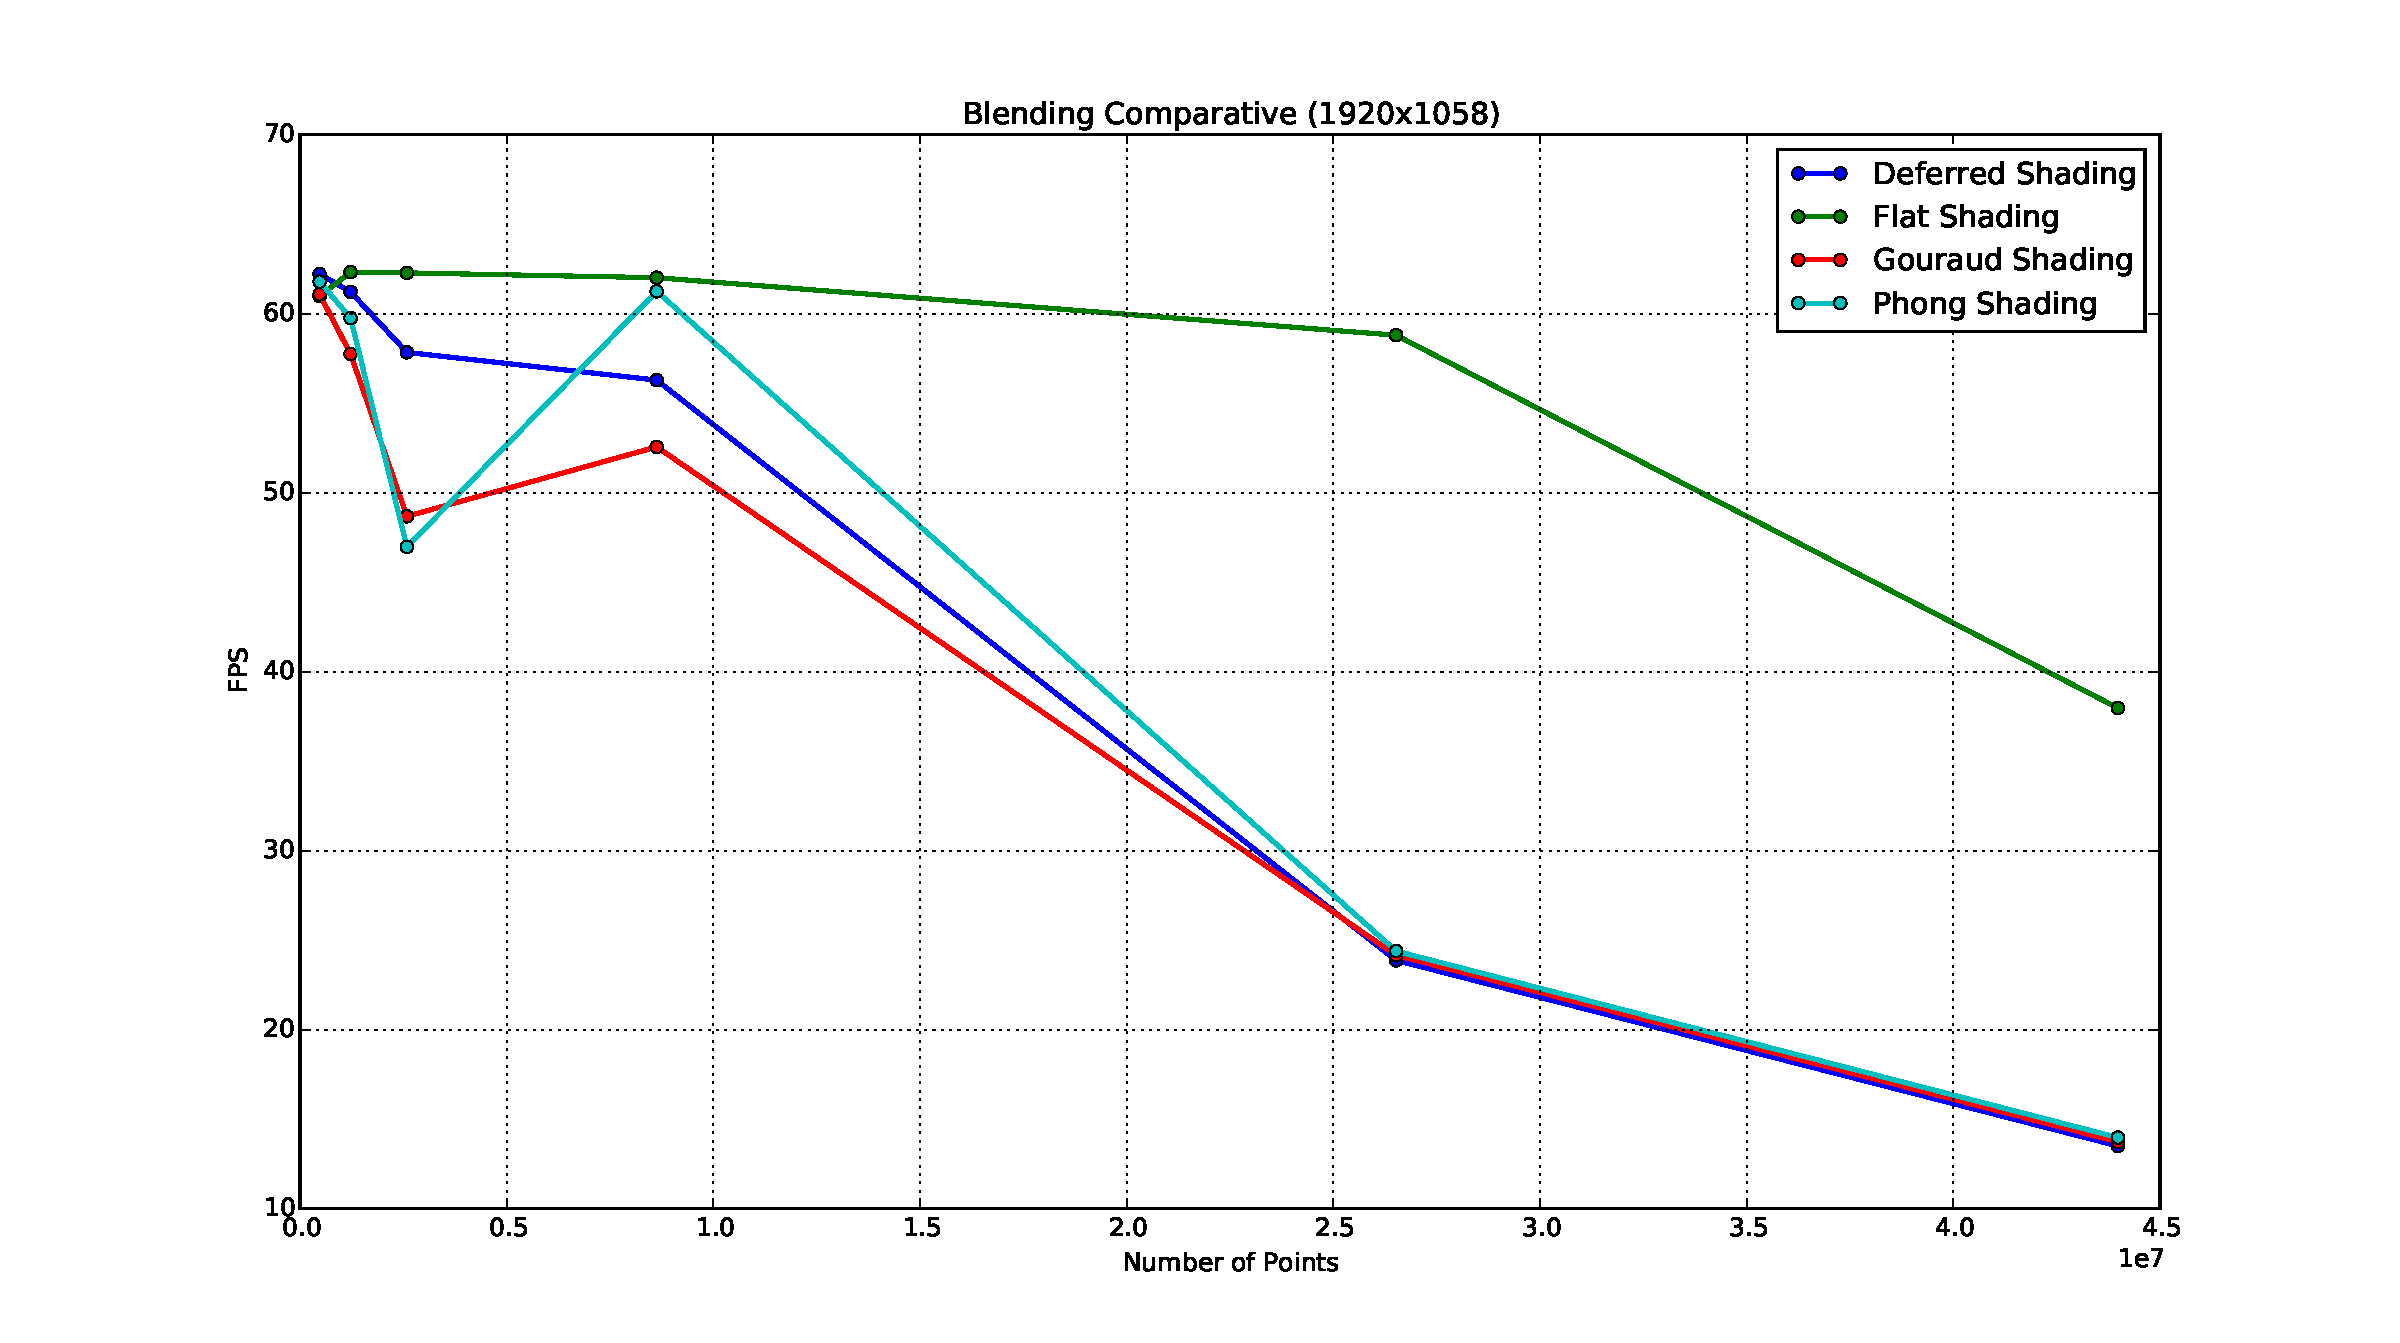
\includegraphics[width=\textwidth]{../figures/blending_graph.pdf}
	\caption{Gr�fica comparativa de los 4 sistemas de blending.}
	\label{figure_blending_graph}
\end{figure}

\subsection[Comparaci�n de los sistemas de blend con puntos de luz] {Comparaci�n de los sistemas de blend con puntos de luz}

Para esta prueba, los seis modelos fueron renderizados con los cuatro algoritmos de \textit{blending} sin antialiasing. Bajo la influencia de diferentes conjuntos de luces radiales. Contando estos conjuntos de un numero de luces variable de 0, 1, 3, 5, 7 o 9 luces. (ver. Figura \ref{figure_blend_vs_light})

Como resultado se concluy� que la iluminaci�n con \textit{Deferred Shading} es mas estable en cuanto se aumentan los puntos de luz. De esta forma se evidencia la superioridad de la iluminaci�n por \textit{pixel} en contrapuesta con los algoritmos que iluminan por \textit{fragmento}.

\begin{figure}    
	\centering
    \subcaptionbox{Flat Shading} {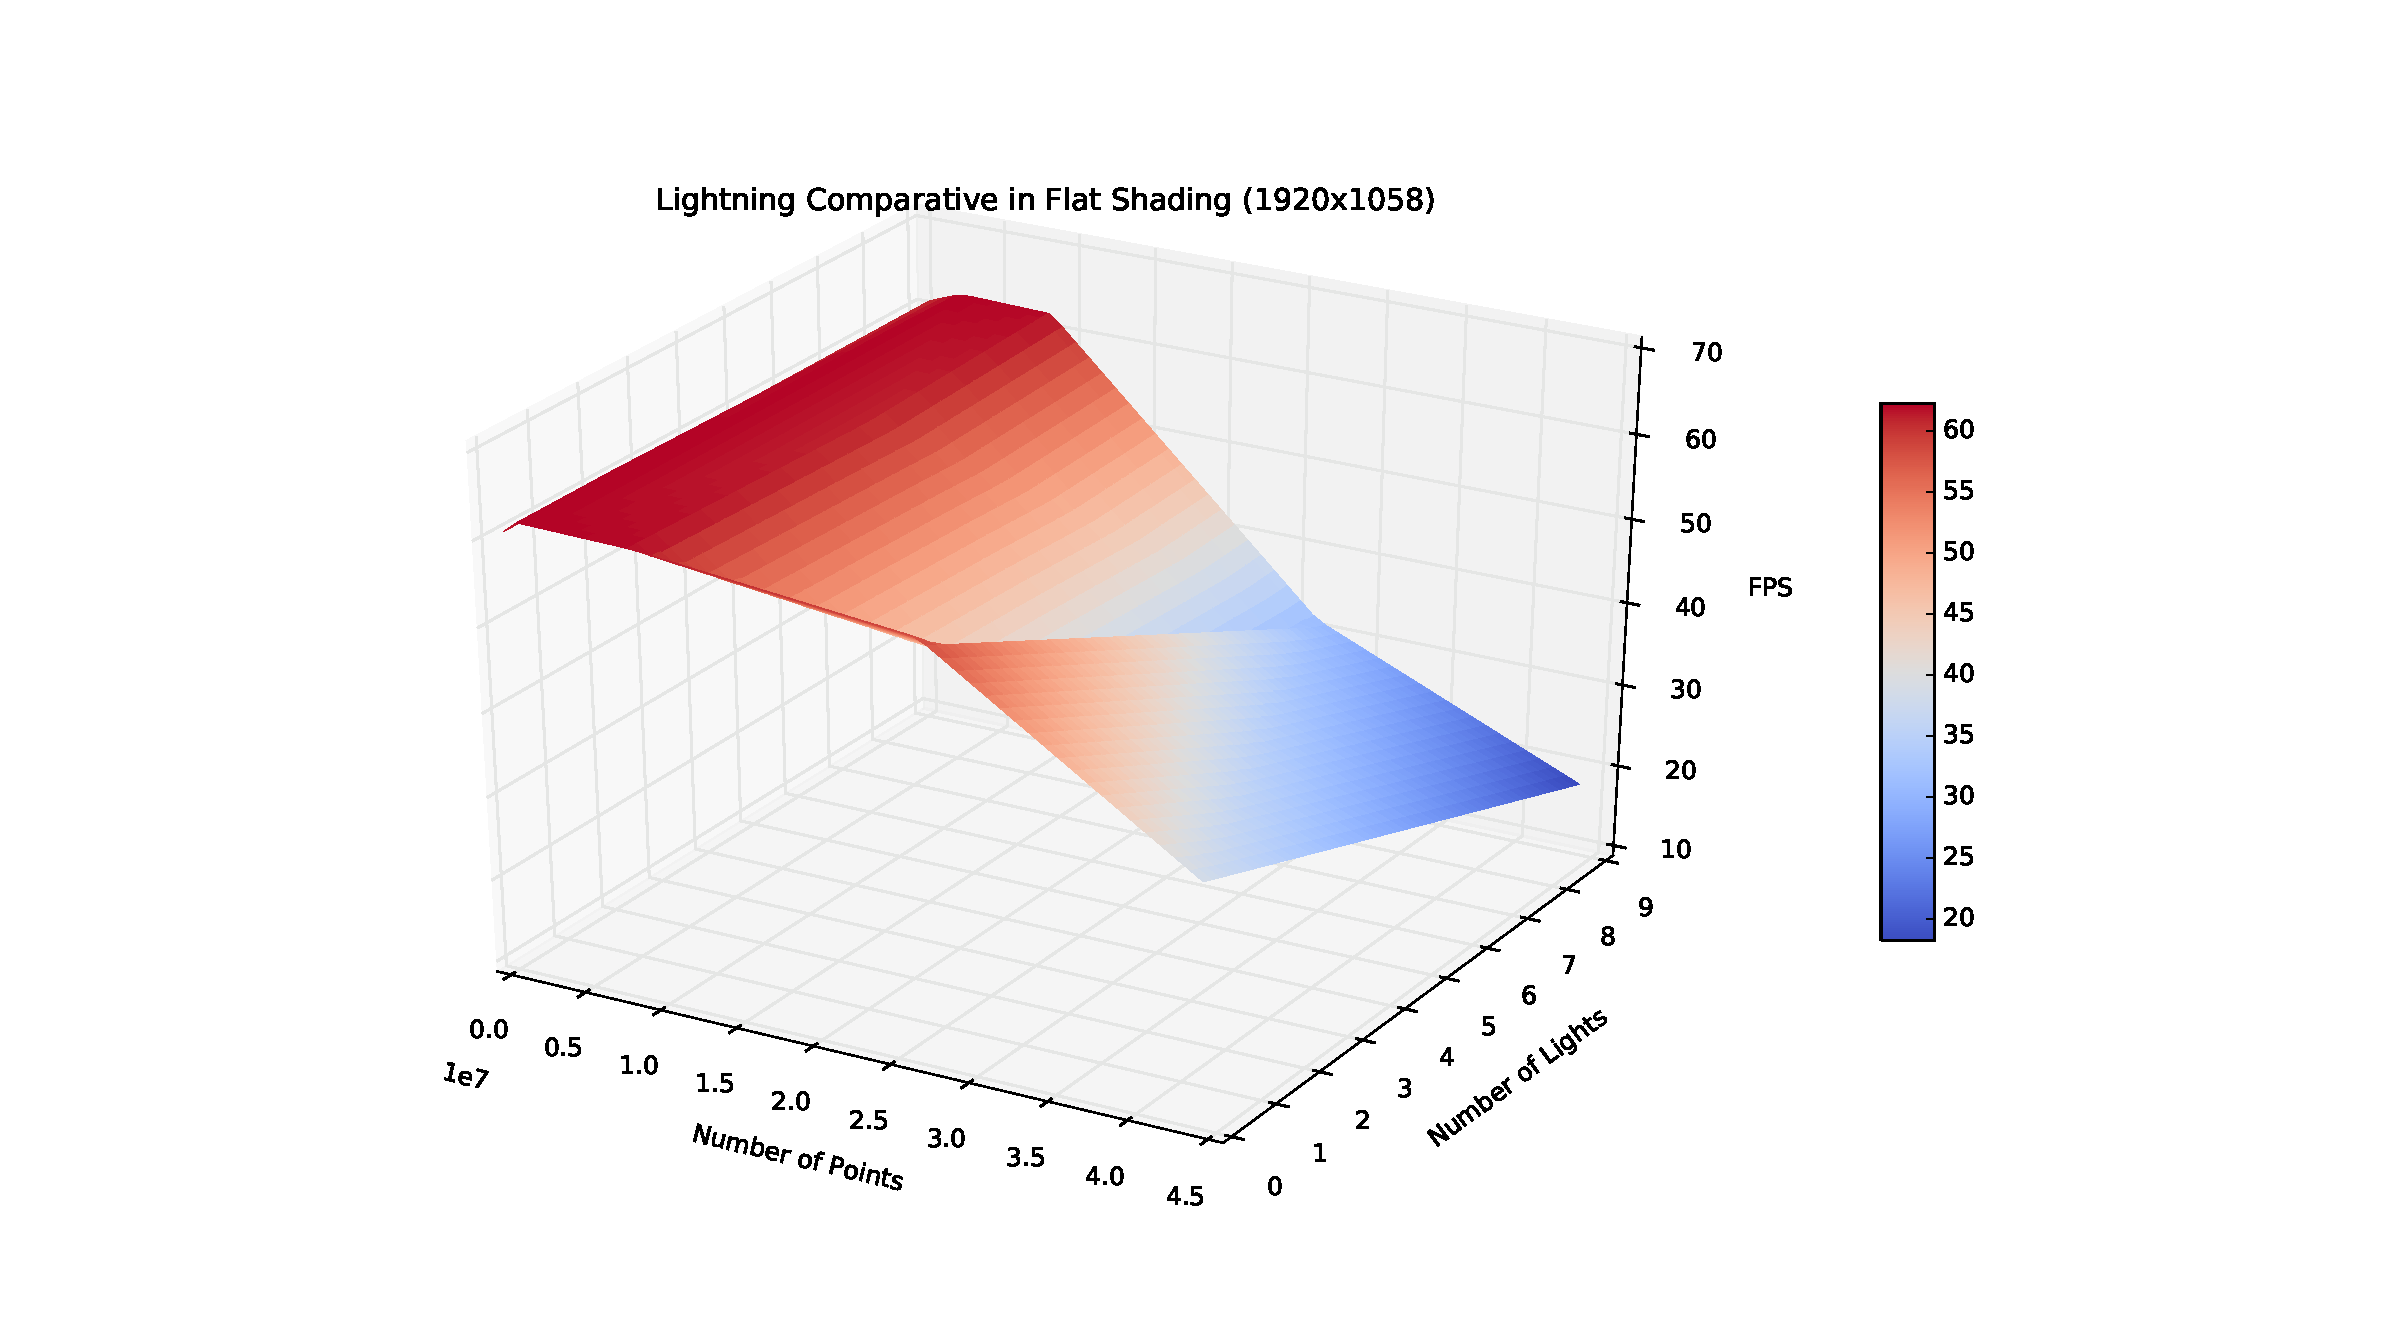
\includegraphics[width=0.48\columnwidth]{../figures/flat_graph.pdf}}    
    \subcaptionbox{Gouraud Shading} {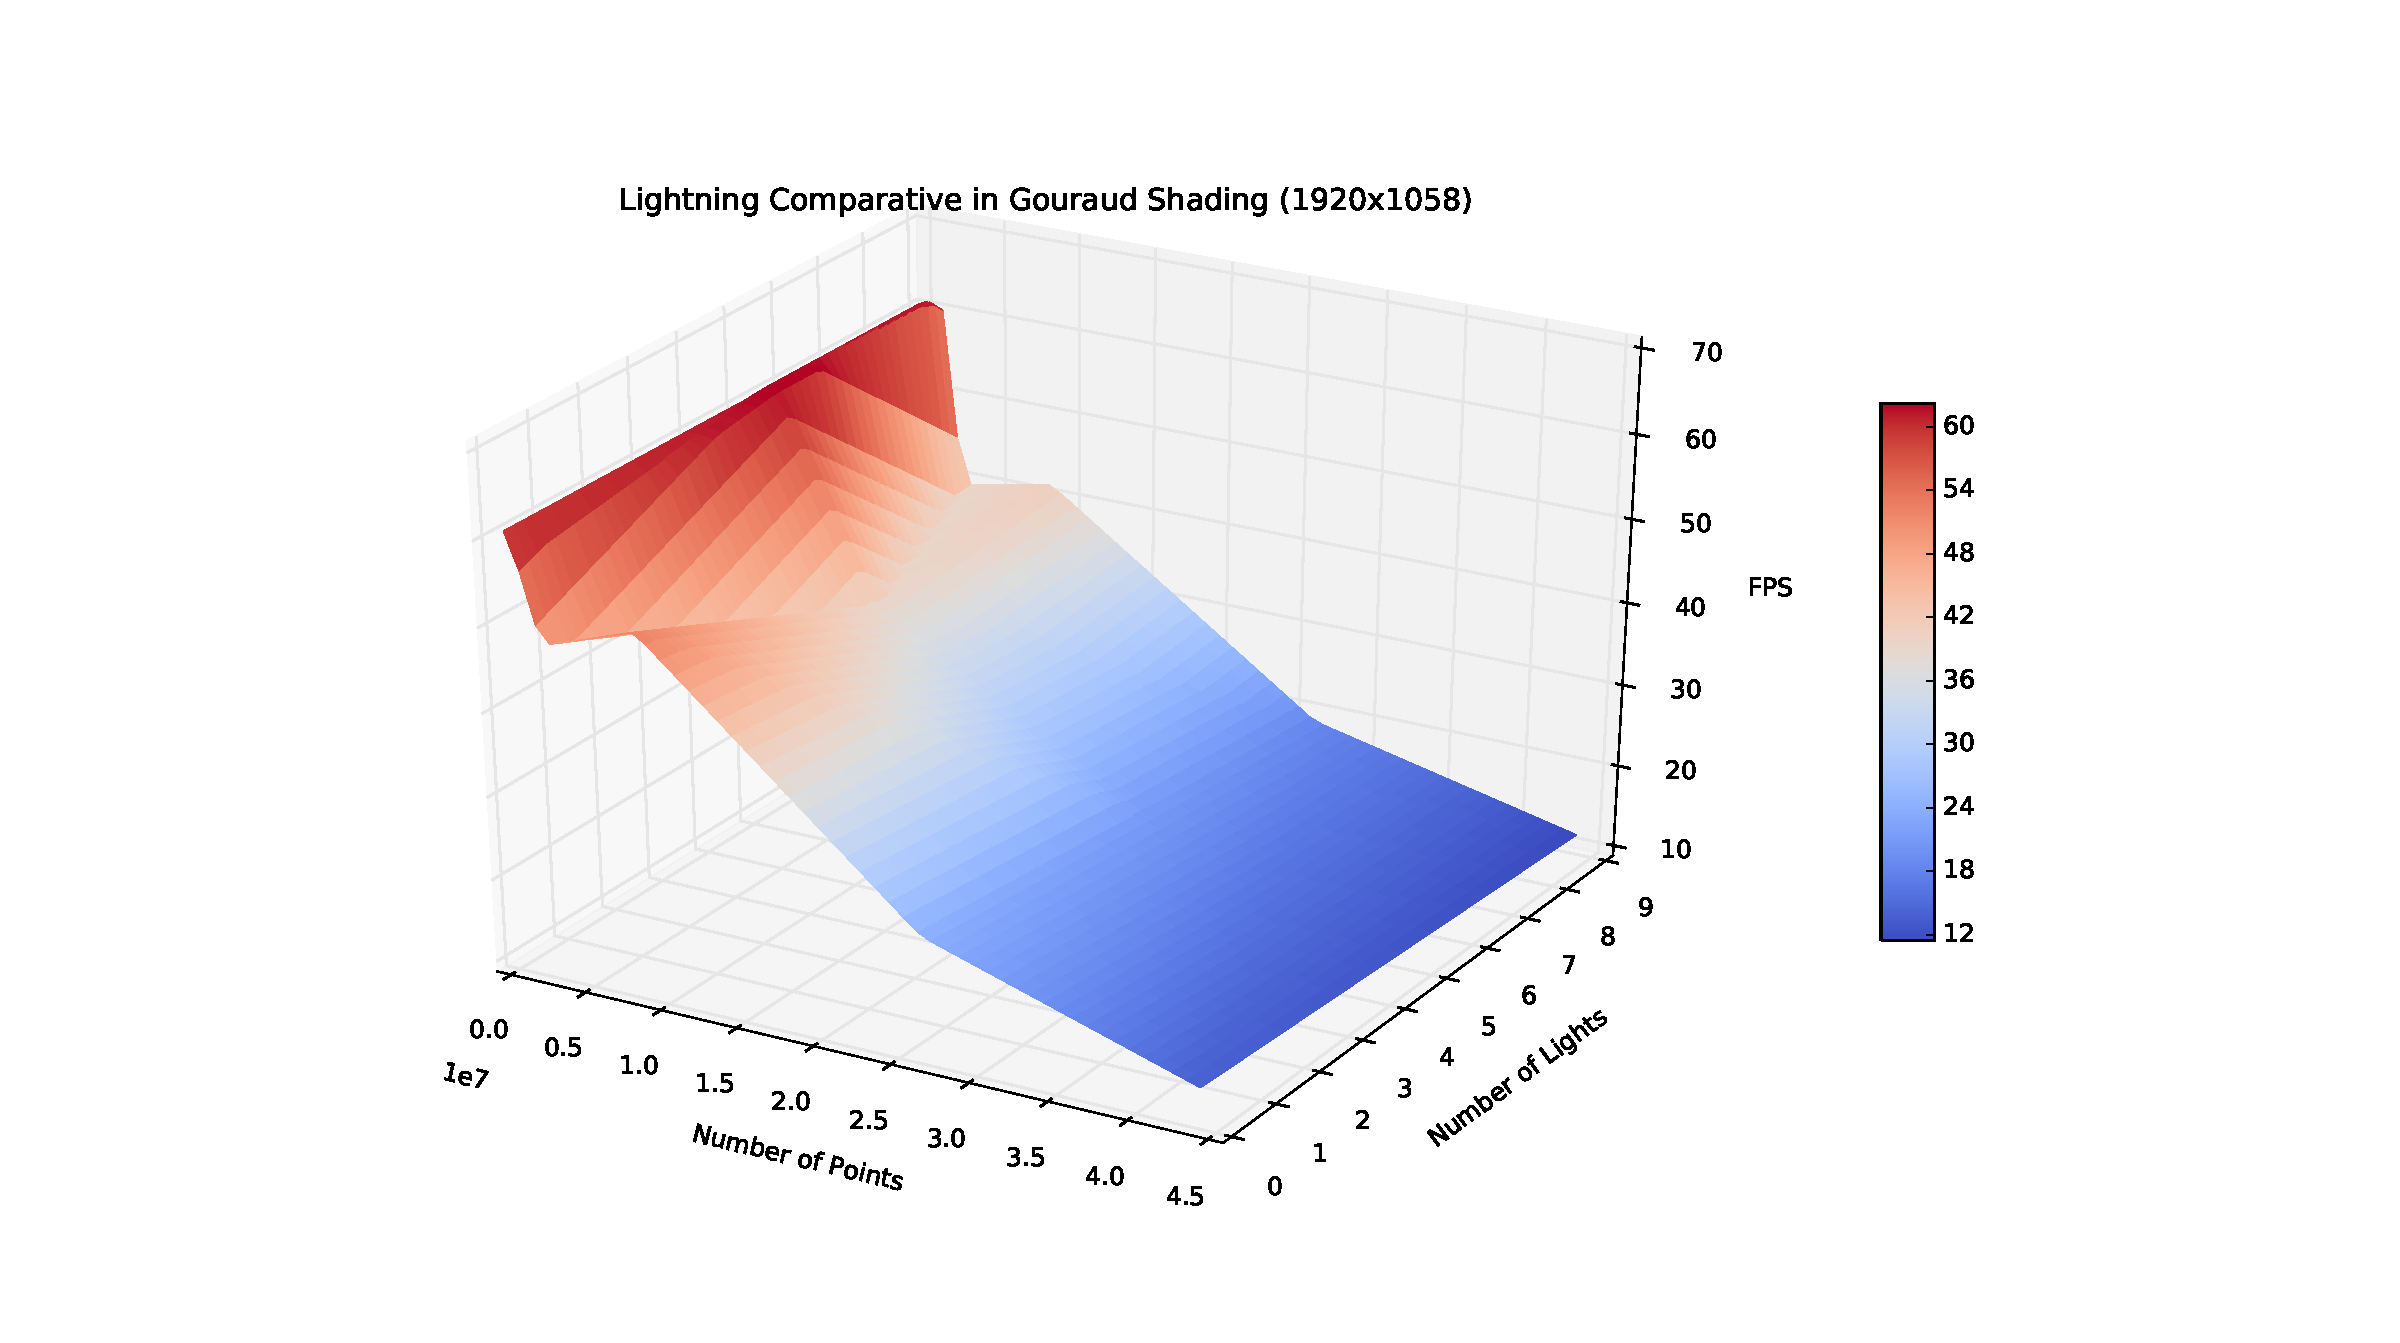
\includegraphics[width=0.48\columnwidth]{../figures/gouraud_graph.pdf}}
    \subcaptionbox{Phong Shading} {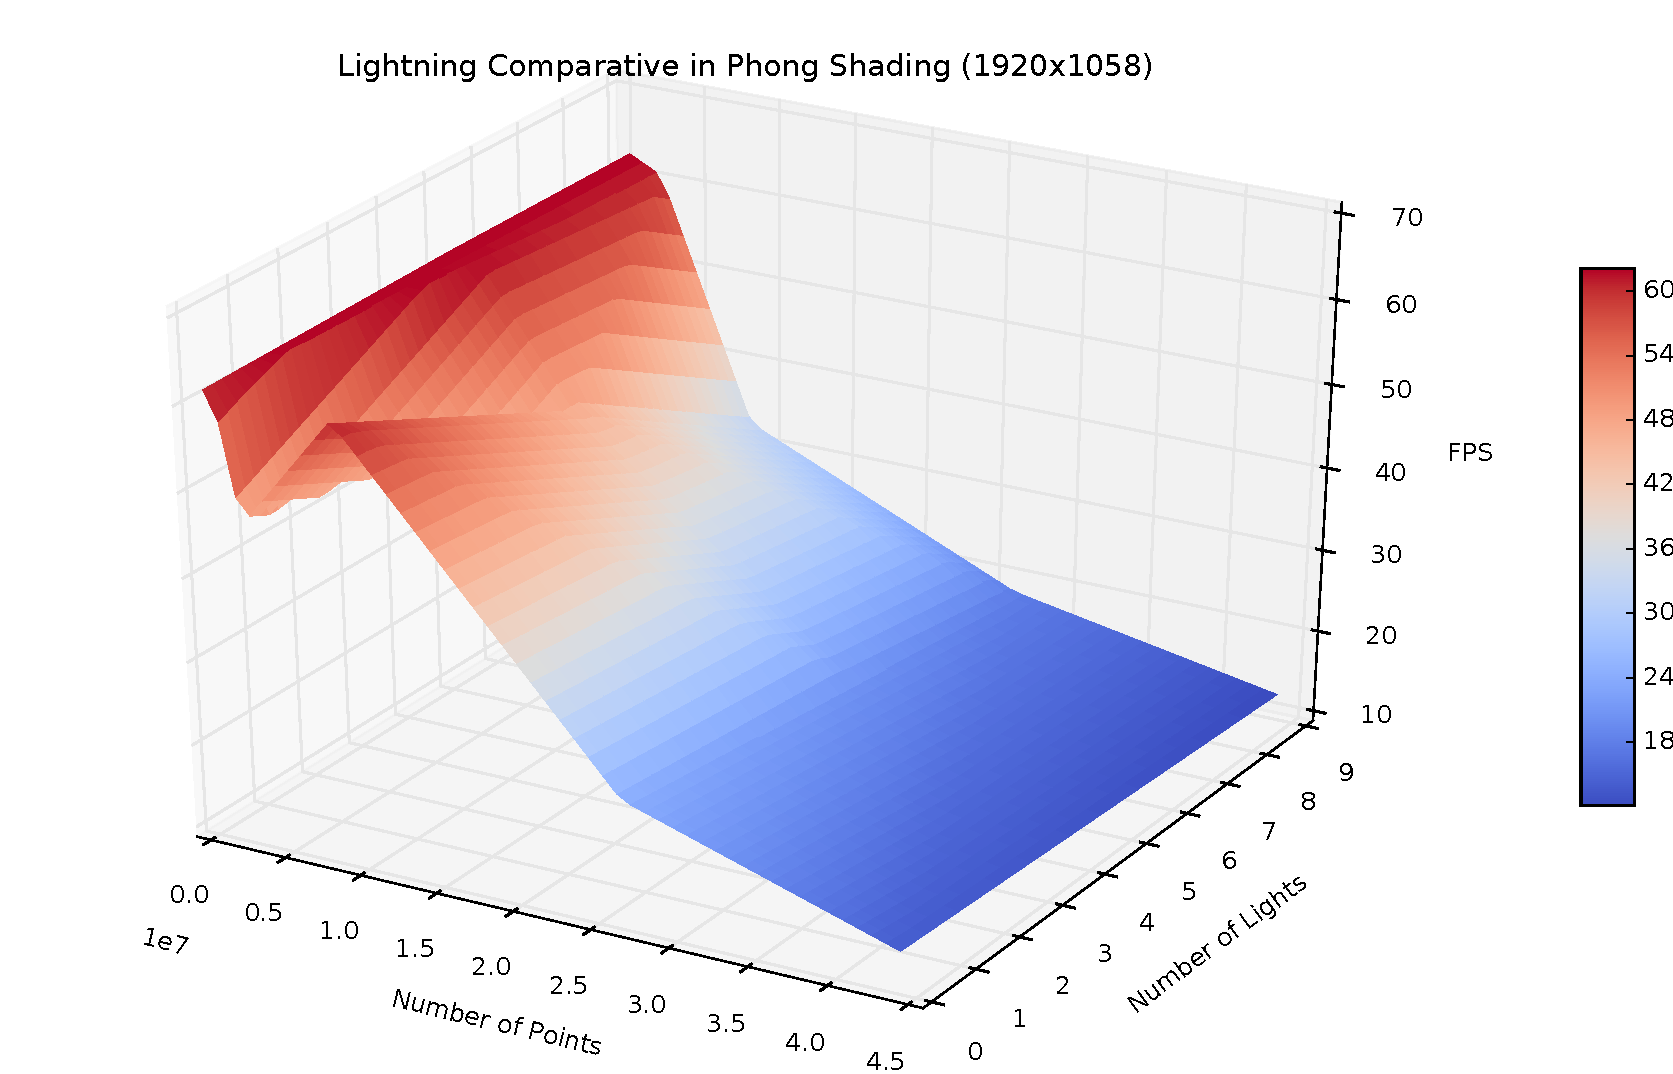
\includegraphics[width=0.48\columnwidth]{../figures/phong_graph.pdf}} 
    \subcaptionbox{Deferred Shading} {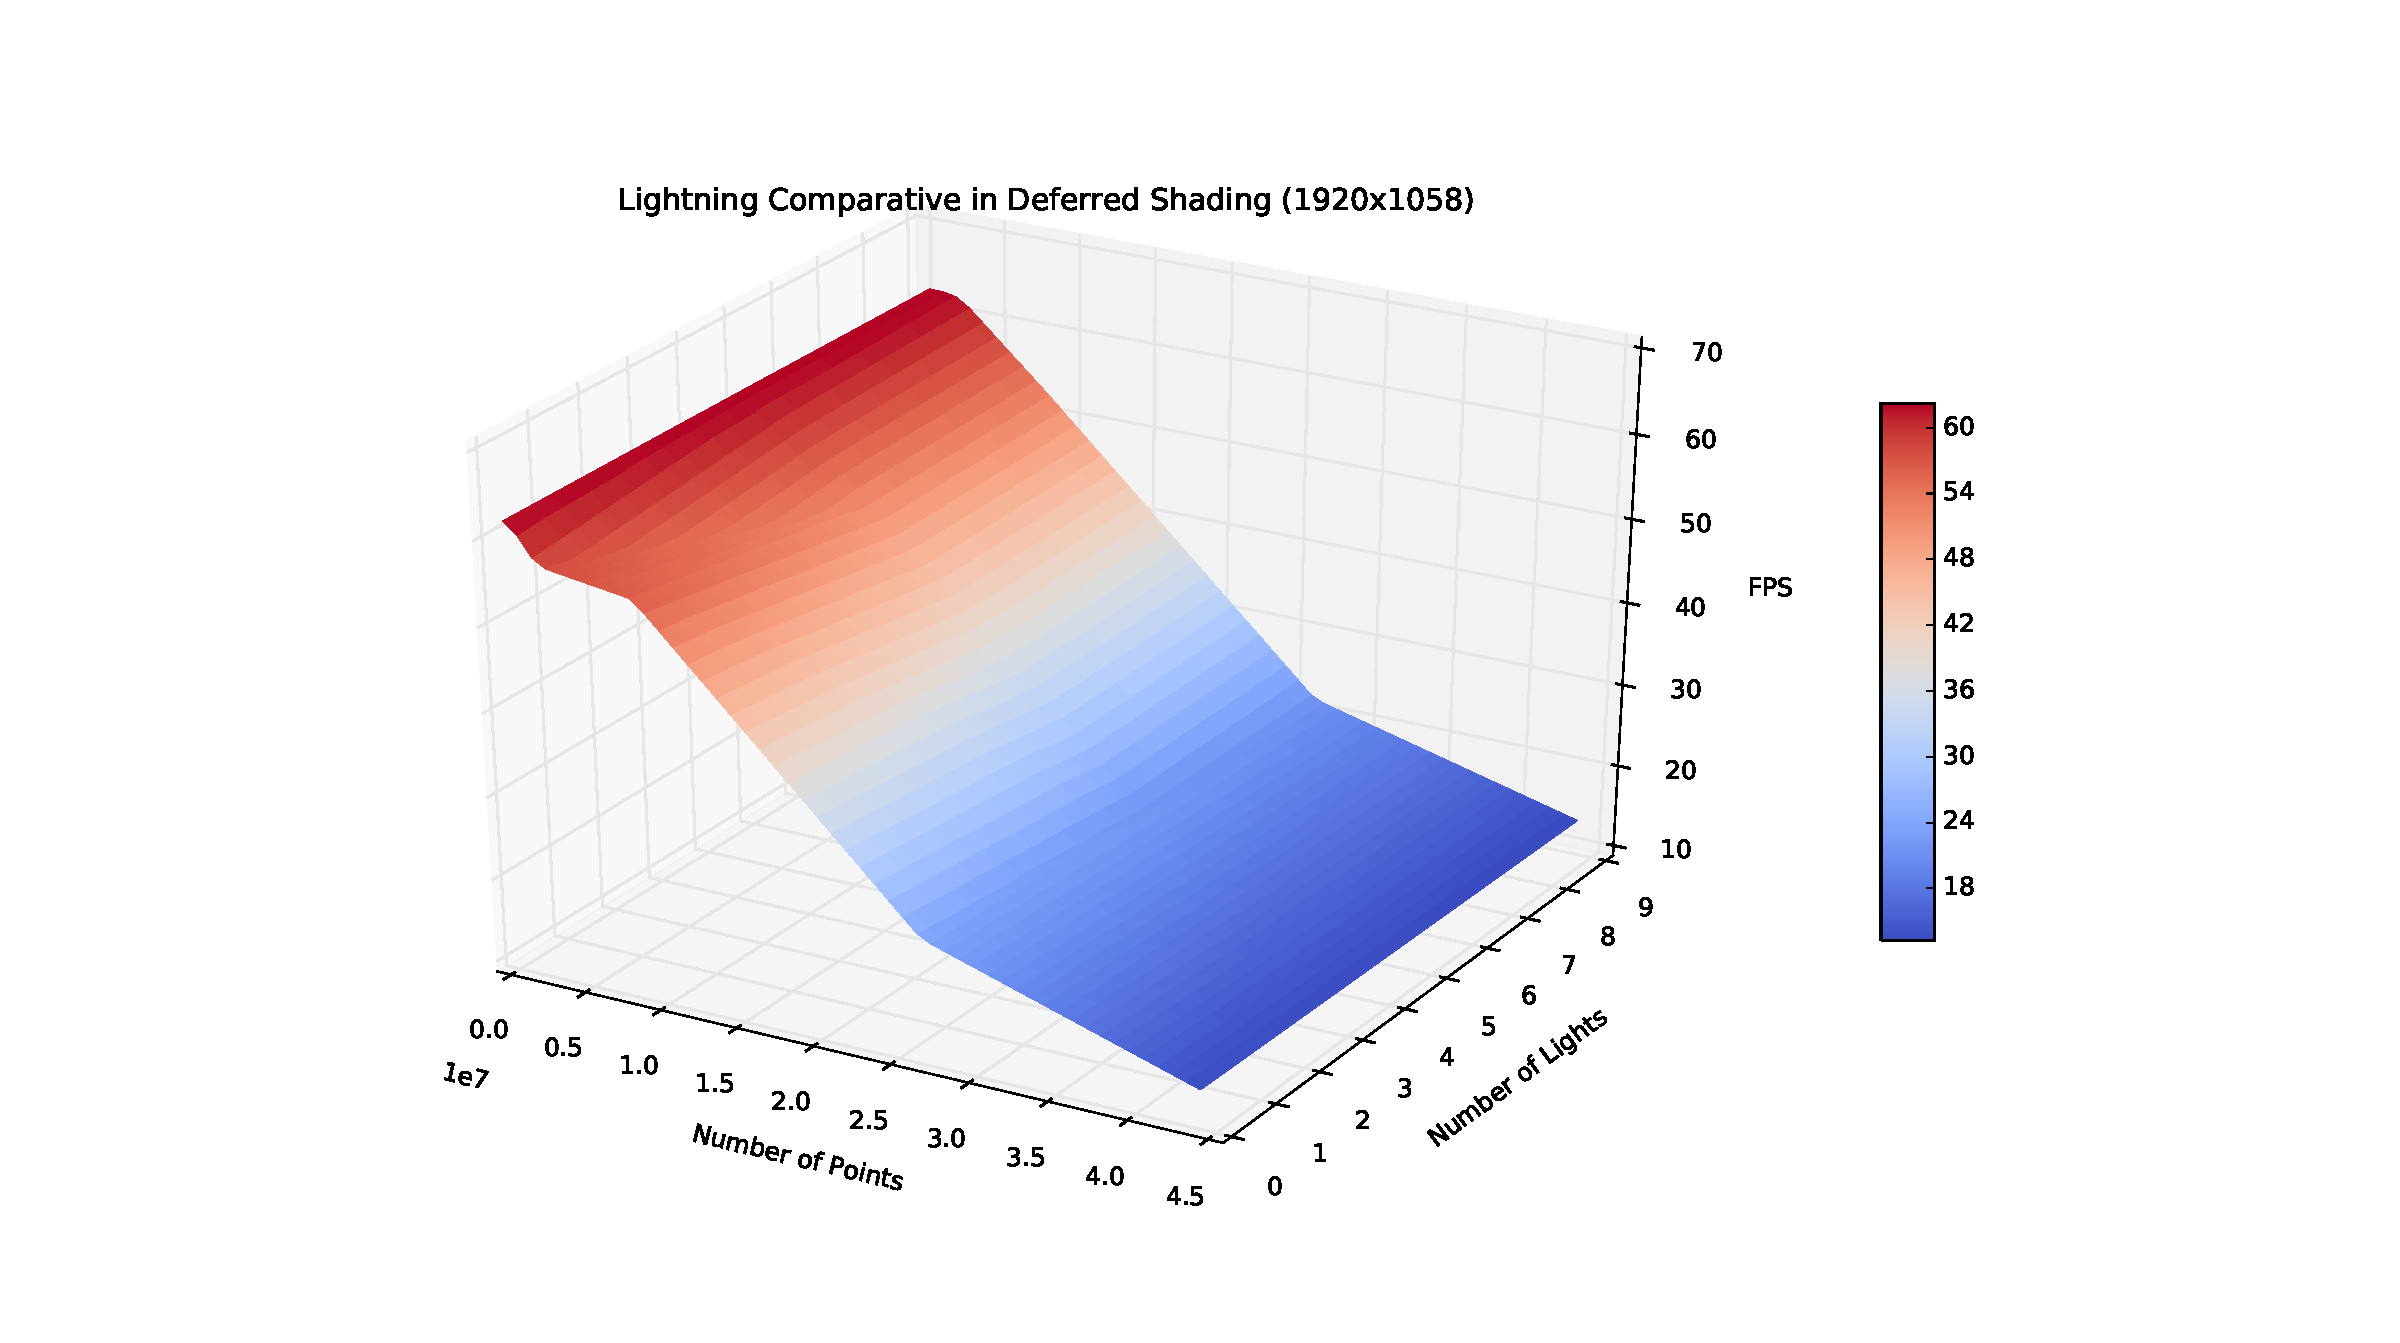
\includegraphics[width=0.48\columnwidth]{../figures/deferred_graph.pdf}} 
	\caption{Comparaci�n de los diferentes sistemas de blending, comparando luces con millones de puntos.}
	\label{figure_blend_vs_light}
\end{figure}


%
% FIN DEL CAP�TULO
%
	%
% CONCLUSIONES
%
\chapter{
	Conclusiones
	\label{nombre_referencia_al_capitulo_070}
}

En este cap�tulo se comentan brevemente las principales conclusiones alcanzadas luego de la finalizaci�n de este Proyecto Fin de Carrera, continuando con las posibles lineas de trabajo que se podr�an derivar del mismo.

\section{Conclusiones}

En relaci�n a las metas fijadas antes del comienzo del proyecto, se podr�a decir que los siguientes objetivos fueron alcanzados:
\begin{itemize}
	\item Aprendizaje en el uso de una librer�a gr�fica como OpenGL.
	\item Programaci�n de programas para GPU con GLSL.
	\item Implementaci�n de un visualizador multiplataforma de modelos de puntos en tiempo real, que sirviera para el prop�sito de estudiar los diferentes algoritmos en \textit{GPU} que existen para su \emph{render}.
	\item Dise�o de herramientas para el an�lisis de resultados mediante lenguajes �giles.
\end{itemize}

Luego de la finalizaci�n de este proyecto, estas son las principales conclusiones alcanzadas en relaci�n a la visualizi�n de las nubes de puntos:
\begin{itemize}
	\item \textbf{El mismo tama�o para todos los puntos es un error:} El tiempo necesario para calcular como m�nimo la correcci�n de profundidad garantiza un mejora en la percepci�n visual adem�s de mejoras en el tiempo de renderizado para nubes de alta densidad. 
	
	\item \textbf{El aumento en la cantidad de puntos no siempre es mejor:} Al representar nubes con una muy alta densidad de puntos, implica un aumento desproporcionado del esfuerzo computacional necesario para acabar en muchos de los casos con resultados semejantes al renderizado con algoritmos simples. Incluso provocando que los algoritmos de \textit{blending} no tengan efecto al probocar superfices de solape �nfimas impidiendo que funcionen los algoritmos correctamente.
	
	\item \textbf{Investigar en sistemas de render que no usen normales:} A pesar de que los resultados obtenidos del render mediante algoritmos como \textit{deferred} son muy buenos. Las nubes de puntos en mucho de los \textit{datasets} carecen de este dato. Por lo que se exige de una precomputaci�n que una vez superando cierto tama�o empieza a no ser abordable, adem�s de que las normales obtenidas en muchos de los casos son erroneas probocando que las im�genes resultantes no se vean correctamente.
	
\end{itemize} 

\section[Posibles v�as de desarrollo]{Posibles v�as de desarrollo}

Con la finalizaci�n del desarrollo de este proyecto, surgen diferentes ideas para continuar con el trabajo iniciado en el mismo:

\begin{itemize}
	\item \textbf{Rendimiento:} A pesar de que se intent� que el rendimiento obtenido del programa fuera lo m�s eficiente posible, habr�a que repasar y analizar bien las especificaciones del \textit{hardware} gr�fico para que las transacciones de datos fuera mas eficientes, intentando evitar sobrecomputaci�n evitable con buenas praxis.
 
	\item \textbf{Interfaz de usuario:} Hacer una migraci�n de \textit{GLFW} a \textit{Qt} con la idea de a�adir una interfaz de usuario y poder ofrecer m�s informaci�n y opciones al usuario.
	
	\item \textbf{Shaders:} Permitir al usuario el escribir sus propios shaders y probarlos online con los modelos cargados.
	
	\item \textbf{C�mara:} Mejorar el funcionamiento de la c�mara orbital, adem�s de a�adir mejoras en esta para poder moverse con m�s libertad por la escena.

	\item \textbf{Frustum culling:} Ahora mismo todos los puntos de la nube son enviados a GPU, ser�a interesante en desarrollar alg�n sistema para filtrar  estos datos mediante alg�n m�todo de \textit{hashing} espacial en funci�n de la c�mara antes de ser enviados para dibujar.
	
	\item \textbf{Order-independent transparency:} Implementar un sistema para intentar simplificar el \textit{blending} en tres pases a un sistema en un �nico pase que adem�s pueda ser aplicado a todos los algoritmos de rasterizaci�n.
	
\end{itemize}
%
% FIN DEL CAP�TULO
%



	% INCLUIMOS LOS AP�NDICES...
    %    \appendix
	%%
% Apendice de shaders
%

\chapter[Shaders]{Shaders.}

\section{Sized-Fixed Points \label{sized-fixed}}

\textbf{Vertex Shader}
\begin{lstlisting}[frame=single]
#version 400
uniform mat4 viewMatrix, projMatrix;
uniform mat3 normalMatrix;

in  vec3 in_Position;
in  vec3 in_Color;

out vec3 ex_Color;

void main(void) {
	gl_Position = projMatrix * viewMatrix * vec4(in_Position, 1.0);
	gl_PointSize = 2;

	vec3 color = vec3 (0.0, 0.0f, 0.0f);

	ex_Color = in_Color;
}
\end{lstlisting}

\textbf{Fragment Shader}
\begin{lstlisting}[frame=single]
#version 400
in  vec3 ex_Color;
out vec4 out_Color;

void main(void) {	
	out_Color = vec4(ex_Color,1.0);
}
\end{lstlisting}
\vfill

\section{Image-aligned Squares \label{image-aligned}}
\textbf{Vertex Shader}
\begin{lstlisting}[frame=single]
#version 400
uniform mat4 viewMatrix, projMatrix;
uniform mat3 normalMatrix;
uniform int h; //Height of the viewport
uniform float n; //Near parameter of the viewing frustum
uniform float t; //Top parameter of the viewing frustum
uniform float b; //Bottom parameter of the viewing frustum

in float in_Radius;
in  vec3 in_Position;
in  vec3 in_Color;

out float ex_Radius;
out vec3 ex_Color;

vec4 ccPosition; //position in Camera Coordinates

void main(void) {

	ex_Radius = in_Radius;

	ccPosition = viewMatrix * vec4(in_Position, 1.0);
	gl_Position = projMatrix * ccPosition;
	gl_PointSize = 2 * ex_Radius * (n / ccPosition.z) * (h / (t-b));

	vec3 color = vec3 (0.0, 0.0f, 0.0f);

	ex_Color = in_Color;
}
\end{lstlisting}

\textbf{Fragment Shader}
\begin{lstlisting}[frame=single]
#version 400
uniform float n; //Near parameter of the viewing frustum
uniform float f; //Far parameter of the viewing frustum

in  vec3 ex_Color;
out vec4 out_Color;

void main(void)
{	
	out_Color = vec4(ex_Color,1.0);
}
\end{lstlisting}
\vfill


\section{Affinely Projected Point Sprites \label{affinely}}
\textbf{Vertex Shader}
\begin{lstlisting}[frame=single]
#version 400
uniform mat4 viewMatrix, projMatrix;
uniform mat3 normalMatrix;
uniform int h; //Height of the viewport
uniform float n; //Near parameter of the viewing frustum
uniform float t; //Top parameter of the viewing frustum
uniform float b; //Bottom parameter of the viewing frustum

in float in_Radius;
in  vec3 in_Position;
in  vec3 in_Color;
in 	vec3 in_Normals;

out float ex_Radius;
out vec3 ex_Color;
out vec3 ex_Normals;
out float ex_Pz; //z in Camera Coordinates

vec4 ccPosition; //position in Camera Coordinates

void main(void) {
	ex_Normals = normalize(normalMatrix * in_Normals);

	if (abs(ex_Normals.z) <= 0.1)
		ex_Normals.z = 0.1;

	ex_Radius = in_Radius;

	ccPosition = viewMatrix * vec4(in_Position, 1.0);
	gl_Position = projMatrix * ccPosition;
	gl_PointSize = 2*ex_Radius * (n / ccPosition.z) * (h / (t-b));

	//BackFace Culling
	if (dot (ccPosition.xyz, ex_Normals) > 0)
		gl_Position.w = 0;

	vec3 color = vec3 (0.0, 0.0f, 0.0f);

	ex_Color = in_Color;

	ex_Pz = ccPosition.z;
}
\end{lstlisting}

\textbf{Fragment Shader}
\begin{lstlisting} [frame=single]
#version 400
uniform float n; //Near parameter of the viewing frustum
uniform float f; //Far parameter of the viewing frustum

in  vec3 ex_Color;
in 	vec3 ex_Normals;
in float ex_Pz;

out vec4 out_Color;

vec3 test;
float zBuffer;

void main(void) {
	test.x = gl_PointCoord.x - 0.5;
	test.y = gl_PointCoord.y - 0.5;
	test.z = -(ex_Normals.x/ex_Normals.z) * test.x - (ex_Normals.y/ex_Normals.z) * test.y;
	if (length(test) > 0.5)
		discard;

	zBuffer = (ex_Pz + test.z * 0.1);
	gl_FragDepth = ((1.0 / zBuffer) * ( (f * n) / (f - n) ) + ( f / (f - n) ));
	
	out_Color = vec4(ex_Color,1.0);
}
\end{lstlisting}
\vfill

\section{Perspective Correct Rasterization \label{perspective}}

\textbf{Vertex Shader}
\begin{lstlisting} [frame=single]
#version 400
uniform mat4 viewMatrix, projMatrix;
uniform mat3 normalMatrix;
uniform int h; //Height of the viewport
uniform float n; //Near parameter of the viewing frustum
uniform float t; //Top parameter of the viewing frustum
uniform float b; //Bottom parameter of the viewing frustum
uniform float userRadiusFactor; //Splat's radii
uniform bool automaticRadiusEnabled;

in float in_Radius;
in  vec3 in_Position;
in  vec3 in_Color;
in 	vec3 in_Normals;

out vec3 ex_Color;
out float ex_Radius;

out vec4 ccPosition; //position in Camera Coordinates
out vec3 normals;



void main(void) {
	normals = normalize(normalMatrix * in_Normals);

	ex_Radius = in_Radius;

	ccPosition = viewMatrix * vec4(in_Position, 1.0);
	gl_Position = projMatrix * ccPosition;
	gl_PointSize = 2 * ex_Radius * (n / ccPosition.z) * (h / (t-b));

	//BackFace Culling
	if (dot (ccPosition.xyz, normals) > 0)
		gl_Position.w = 0;

	ex_Color = in_Color;
}
\end{lstlisting}
\newpage
\textbf{Fragment Shader}
\begin{lstlisting} [frame=single]
#version 400
uniform mat4 viewMatrix;
uniform float n; //Near parameter of the viewing frustum
uniform float f; //Far parameter of the viewing frustum
uniform float t; //Top parameter of the viewing frustum
uniform float b; //Bottom parameter of the viewing frustum
uniform float r; //Right parameter of the viewing frustum
uniform float l; //Left parameter of the viewing frustum
uniform int h; 	 //Height of the viewport
uniform int w; 	 //Width of the viewport

uniform int lightCount;
uniform vec3 lightPosition[16];
uniform vec3 lightColor[16];
uniform float lightIntensity[16];

in float ex_Radius;
in  vec3 ex_Color;
in  vec3 normals;
in 	vec4 ccPosition;

out vec4 out_Color;

void main(void) {

	vec3 qn;
	qn.x = (gl_FragCoord.x ) *  ((r - l)/w ) - ( (r - l)/2.0 );
	qn.y = (gl_FragCoord.y ) *  ((b - t)/h ) - ( (b - t)/2.0 );
	qn.z = -n;

	float denom = dot (qn, normals);

	if (denom == 0.0)
		discard;

	float timef = dot (ccPosition.xyz, normals ) / denom;

	vec3 q = qn * timef;
	vec3 testq = q;
	
	vec3 dist = (q - ccPosition.xyz);

	if ((dist.x * dist.x) + (dist.y * dist.y) + (dist.z * dist.z) > pow(ex_Radius, 2))
		discard;

	gl_FragDepth = ((1.0 / q.z) * ( (f * n) / (f - n) ) + ( f / (f - n) ));

	out_Color = vec4(ex_Color, 1.0f);
}
\end{lstlisting}
\newpage

\section{Gouraud \label{gouraud}}
\subsection{Visibility Pass}
\textbf{Vertex Shader}
\begin{lstlisting} [frame=single]
#version 410
uniform mat4 viewMatrix, projMatrix;
uniform mat3 normalMatrix;
uniform int h; //Height of the viewport
uniform float n; //Near parameter of the viewing frustum
uniform float t; //Top parameter of the viewing frustum
uniform float b; //Bottom parameter of the viewing frustum

in  vec3 in_Position;
in 	vec3 in_Normals;
in  float in_Radius;

out float ex_Radius;

out vec4 ccPosition; //position in Camera Coordinates
out vec3 normals;


void main(void) {

	ex_Radius = in_Radius;

	normals = normalize(normalMatrix * in_Normals);

	ccPosition = viewMatrix * vec4(in_Position, 1.0);
	gl_Position = projMatrix * ccPosition;
	gl_PointSize = 2 * ex_Radius * (n / ccPosition.z) * (h / (t-b));
}
\end{lstlisting}
\newpage

\textbf{Fragment Shader}
\begin{lstlisting} [frame=single]
#version 410
uniform float n; //Near parameter of the viewing frustum
uniform float f; //Far parameter of the viewing frustum
uniform float t; //Top parameter of the viewing frustum
uniform float b; //Bottom parameter of the viewing frustum
uniform float r; //Right parameter of the viewing frustum
uniform float l; //Left parameter of the viewing frustum
uniform int h; 	 //Height of the viewport
uniform int w; 	 //Width of the viewport

in float ex_Radius;
in  vec3 normals;
in 	vec4 ccPosition;

void main(void) {

	vec3 qn;
	qn.x = (gl_FragCoord.x ) *  ((r - l)/w ) - ( (r - l)/2.0 );
	qn.y = (gl_FragCoord.y ) *  ((b - t)/h ) - ( (b - t)/2.0 );
	qn.z = -n;

	float denom = dot (qn, normals);

	if (denom == 0.0)
		discard;

	float timef = dot (ccPosition.xyz, normals ) / denom;

	vec3 q = qn * timef;
	
	vec3 dist = (q - ccPosition.xyz);

	if ((dist.x * dist.x) + (dist.y * dist.y) + (dist.z * dist.z) > pow(ex_Radius, 2))
		discard;

	gl_FragDepth = ((1.0 / q.z) * ( (f * n) / (f - n) ) + ( f / (f - n) ));

}
\end{lstlisting}
\newpage

\subsection{Blending Pass}
\textbf{Vertex Shader}
\begin{lstlisting} [frame=single]
#version 410
uniform mat4 viewMatrix, projMatrix;
uniform mat3 normalMatrix;
uniform int h; //Height of the viewport
uniform float n; //Near parameter of the viewing frustum
uniform float t; //Top parameter of the viewing frustum
uniform float b; //Bottom parameter of the viewing frustum

in float in_Radius;
in  vec3 in_Position;
in  vec3 in_Color;
in 	vec3 in_Normals;

out vec3 ex_Color;
out float ex_Radius;

out vec4 ccPosition; //position in Camera Coordinates
out vec3 normals;

void main(void) {
	normals = normalize(normalMatrix * in_Normals);

	ex_Radius = in_Radius;

	ccPosition = viewMatrix * vec4(in_Position, 1.0);
	gl_Position = projMatrix * ccPosition;
	gl_PointSize = 2*ex_Radius * (n / ccPosition.z) * (h / (t-b));

	//Backface Culling
	if (dot (ccPosition.xyz, normals) > 0)
		gl_Position.w = 0;

	ex_Color = in_Color;
}
\end{lstlisting}

\textbf{Fragment Shader}
\begin{lstlisting} [frame=single]
#version 410
uniform mat4 viewMatrix;
uniform float n; //Near parameter of the viewing frustum
uniform float f; //Far parameter of the viewing frustum
uniform float t; //Top parameter of the viewing frustum
uniform float b; //Bottom parameter of the viewing frustum
uniform float r; //Right parameter of the viewing frustum
uniform float l; //Left parameter of the viewing frustum
uniform int h; 	 //Height of the viewport
uniform int w; 	 //Width of the viewport

uniform int lightCount;
uniform vec3 lightPosition[16];
uniform vec3 lightColor[16];
uniform float lightIntensity[16];

in float ex_Radius;
in  vec3 ex_Color;
in 	vec3 ex_UxV;
in  vec3 normals;
in 	vec4 ccPosition;

layout (location = 0) out vec4 out_Color;

void main(void) {

	vec3 qn;
	qn.x = (gl_FragCoord.x ) *  ((r - l)/w ) - ( (r - l)/2.0 );
	qn.y = (gl_FragCoord.y ) *  ((b - t)/h ) - ( (b - t)/2.0 );
	qn.z = -n;

	float denom = dot (qn, normals);

	if (denom == 0.0)
		discard;

	float timef = dot (ccPosition.xyz, normals ) / denom;

	vec3 q = qn * timef;
	vec3 testq = q;

	vec3 dist = (q - ccPosition.xyz);

	if ((dist.x * dist.x) + (dist.y * dist.y) + (dist.z * dist.z) > pow(ex_Radius, 2))
		discard;

	vec3 epsilon = normalize(qn)/40.0f;
	q = q - epsilon;

	gl_FragDepth = ((1.0 / q.z) * ( (f * n) / (f - n) ) + ( f / (f - n) ));
	float weight = (1.0f - length(dist)/ex_Radius);

	vec3 color = ex_Color;

	//Diffuse
	vec3 dotValue = vec3(0,0,0);
	for (int i = 0; i < lightCount; i++) {
		vec3 ccLightPosition = (viewMatrix * vec4(lightPosition[i], 1.0f)).xyz;
		vec3 lithToQ = normalize(ccLightPosition - testq);
		dotValue += vec3(max(dot(normals, lithToQ), 0.0)) * lightIntensity[i] * lightColor[i];
	}

	out_Color = vec4(dotValue + color, 1.0f);
}
\end{lstlisting}
\newpage

\subsection{Normalization Pass}
\textbf{Vertex Shader}
\begin{lstlisting} [frame=single]
#version 410
in  vec3 in_Position;
in 	vec3 in_Color;

out vec4 out_Color;

void main(void)
{
	gl_Position = vec4(in_Position, 1.0);
}
\end{lstlisting}

\textbf{Fragment Shader}
\begin{lstlisting} [frame=single]
#version 410
uniform sampler2DRect blendTexture;

out vec4 out_Color;

void main(void) {
	vec4 textureColor = texture(blendTexture, gl_FragCoord.xy);

	if (textureColor.a <= 0.0f)
		discard;

	out_Color = vec4(textureColor.rgb/textureColor.a, 1.0f);
}
\end{lstlisting}
\newpage

\section{Phong \label{phong}}
\subsection{Visibility Pass}
\textbf{Vertex Shader}
\begin{lstlisting} [frame=single]
#version 410
uniform mat4 viewMatrix, projMatrix;
uniform mat3 normalMatrix;
uniform int h; //Height of the viewport
uniform float n; //Near parameter of the viewing frustum
uniform float t; //Top parameter of the viewing frustum
uniform float b; //Bottom parameter of the viewing frustum

in  vec3 in_Position;
in 	vec3 in_Normals;
in  float in_Radius;

out float ex_Radius;

out vec4 ccPosition; //position in Camera Coordinates
out vec3 normals;


void main(void) {

ex_Radius = in_Radius;

normals = normalize(normalMatrix * in_Normals);

ccPosition = viewMatrix * vec4(in_Position, 1.0);
gl_Position = projMatrix * ccPosition;
gl_PointSize = 2 * ex_Radius * (n / ccPosition.z) * (h / (t-b));
}
\end{lstlisting}
\newpage

\textbf{Fragment Shader}
\begin{lstlisting} [frame=single]
#version 410
uniform float n; //Near parameter of the viewing frustum
uniform float f; //Far parameter of the viewing frustum
uniform float t; //Top parameter of the viewing frustum
uniform float b; //Bottom parameter of the viewing frustum
uniform float r; //Right parameter of the viewing frustum
uniform float l; //Left parameter of the viewing frustum
uniform int h; 	 //Height of the viewport
uniform int w; 	 //Width of the viewport

in float ex_Radius;
in  vec3 normals;
in 	vec4 ccPosition;

void main(void) {

vec3 qn;
qn.x = (gl_FragCoord.x ) *  ((r - l)/w ) - ( (r - l)/2.0 );
qn.y = (gl_FragCoord.y ) *  ((b - t)/h ) - ( (b - t)/2.0 );
qn.z = -n;

float denom = dot (qn, normals);

if (denom == 0.0)
discard;

float timef = dot (ccPosition.xyz, normals ) / denom;

vec3 q = qn * timef;

vec3 dist = (q - ccPosition.xyz);

if ((dist.x * dist.x) + (dist.y * dist.y) + (dist.z * dist.z) > pow(ex_Radius, 2))
discard;

gl_FragDepth = ((1.0 / q.z) * ( (f * n) / (f - n) ) + ( f / (f - n) ));

}
\end{lstlisting}
\newpage

\subsection{Blending Pass}
\textbf{Vertex Shader}
\begin{lstlisting} [frame=single]
#version 400
uniform mat4 viewMatrix, projMatrix;
uniform mat3 normalMatrix;
uniform int h; //Height of the viewport
uniform float n; //Near parameter of the viewing frustum
uniform float t; //Top parameter of the viewing frustum
uniform float b; //Bottom parameter of the viewing frustum

in float in_Radius;
in  vec3 in_Position;
in  vec3 in_Color;
in 	vec3 in_Normals;

out vec3 ex_Color;
out float ex_Radius;

out vec4 ccPosition; //position in Camera Coordinates
out vec3 normals;

void main(void) {
	normals = normalize(normalMatrix * in_Normals);

	ex_Radius = in_Radius;

	//p. 277
	ccPosition = viewMatrix * vec4(in_Position, 1.0);
	gl_Position = projMatrix * ccPosition;
	gl_PointSize = 2 * ex_Radius * (n / ccPosition.z) * (h / (t-b));

	//BackFace Culling
	if (dot (ccPosition.xyz, normals) > 0)
		gl_Position.w = 0;

	ex_Color = in_Color;
}
\end{lstlisting}
\newpage

\textbf{Fragment Shader}
\begin{lstlisting} [frame=single]
#version 400
uniform mat4 viewMatrix;
uniform float n; //Near parameter of the viewing frustum
uniform float f; //Far parameter of the viewing frustum
uniform float t; //Top parameter of the viewing frustum
uniform float b; //Bottom parameter of the viewing frustum
uniform float r; //Right parameter of the viewing frustum
uniform float l; //Left parameter of the viewing frustum
uniform int h; 	 //Height of the viewport
uniform int w; 	 //Width of the viewport
uniform bool colorEnabled;
uniform int lightCount;
uniform vec3 lightPosition[16];
uniform vec3 lightColor[16];
uniform float lightIntensity[16];

in float ex_Radius;
in  vec3 ex_Color;
in 	vec3 ex_UxV;
in  vec3 normals;
in 	vec4 ccPosition;

out vec4 out_Color;

void main(void) {

	vec3 qn;
	qn.x = (gl_FragCoord.x ) *  ((r - l)/w ) - ( (r - l)/2.0 );
	qn.y = (gl_FragCoord.y ) *  ((b - t)/h ) - ( (b - t)/2.0 );
	qn.z = -n;

	float denom = dot (qn, normals);

	if (denom == 0.0)
		discard;

	float timef = dot (ccPosition.xyz, normals ) / denom;

	vec3 q = qn * timef;
	vec3 testq = q;

	vec3 dist = (q - ccPosition.xyz);

	if ((dist.x * dist.x) + (dist.y * dist.y) + (dist.z * dist.z) > pow(ex_Radius, 2))
		discard;

	vec3 epsilon = normalize(qn)/40.0f;
	q = q - epsilon;

	gl_FragDepth = ((1.0 / q.z) * ( (f * n) / (f - n) ) + ( f / (f - n) ));

	//Phong
	float weight = (1.0f - length(dist)/ex_Radius);
	vec3 phongNormal = normalize((q + normals) - ccPosition.xyz);

	vec3 color = ex_Color;
	//Diffuse
	vec3 dotValue = vec3(0,0,0);
	for (int i = 0; i < lightCount; i++) {
		vec3 ccLightPosition = (viewMatrix * vec4(lightPosition[i], 1.0f)).xyz;
		vec3 lithToQ = normalize(ccLightPosition - testq);
	dotValue += vec3(max(dot(normals, lithToQ), 0.0)) * lightIntensity[i] * lightColor[i];
	}

	out_Color = vec4(dotValue + color, 1.0f * weight);

}
\end{lstlisting}
\newpage

\subsection{Normalization Pass}
\textbf{Vertex Shader}
\begin{lstlisting} [frame=single]
#version 410
in  vec3 in_Position;
in 	vec3 in_Color;

out vec4 out_Color;

void main(void)
{
gl_Position = vec4(in_Position, 1.0);
}
\end{lstlisting}

\textbf{Fragment Shader}
\begin{lstlisting} [frame=single]
#version 410
uniform sampler2DRect blendTexture;

out vec4 out_Color;

void main(void) {
vec4 textureColor = texture(blendTexture, gl_FragCoord.xy);

if (textureColor.a <= 0.0f)
discard;

out_Color = vec4(textureColor.rgb/textureColor.a, 1.0f);
}
\end{lstlisting}
\newpage

\section{Deferred \label{deferred}}
\subsection{Visibility Pass}
\textbf{Vertex Shader}
\begin{lstlisting} [frame=single]
#version 410
uniform mat4 viewMatrix, projMatrix;
uniform mat3 normalMatrix;
uniform int h; //Height of the viewport
uniform float n; //Near parameter of the viewing frustum
uniform float t; //Top parameter of the viewing frustum
uniform float b; //Bottom parameter of the viewing frustum

in  vec3 in_Position;
in 	vec3 in_Normals;
in  float in_Radius;

out float ex_Radius;

out vec4 ccPosition; //position in Camera Coordinates
out vec3 normals;


void main(void) {

ex_Radius = in_Radius;

normals = normalize(normalMatrix * in_Normals);

ccPosition = viewMatrix * vec4(in_Position, 1.0);
gl_Position = projMatrix * ccPosition;
gl_PointSize = 2 * ex_Radius * (n / ccPosition.z) * (h / (t-b));
}
\end{lstlisting}
\newpage

\textbf{Fragment Shader}
\begin{lstlisting} [frame=single]
#version 410
uniform float n; //Near parameter of the viewing frustum
uniform float f; //Far parameter of the viewing frustum
uniform float t; //Top parameter of the viewing frustum
uniform float b; //Bottom parameter of the viewing frustum
uniform float r; //Right parameter of the viewing frustum
uniform float l; //Left parameter of the viewing frustum
uniform int h; 	 //Height of the viewport
uniform int w; 	 //Width of the viewport

in float ex_Radius;
in  vec3 normals;
in 	vec4 ccPosition;

layout (location = 1) out vec3 out_Position;

void main(void) {

vec3 qn;
qn.x = (gl_FragCoord.x ) *  ((r - l)/w ) - ( (r - l)/2.0 );
qn.y = (gl_FragCoord.y ) *  ((b - t)/h ) - ( (b - t)/2.0 );
qn.z = -n;

float denom = dot (qn, normals);

if (denom == 0.0)
discard;

float timef = dot (ccPosition.xyz, normals ) / denom;

vec3 q = qn * timef;

vec3 dist = (q - ccPosition.xyz);

if ((dist.x * dist.x) + (dist.y * dist.y) + (dist.z * dist.z) > pow(ex_Radius, 2))
discard;

out_Position = q;
gl_FragDepth = ((1.0 / q.z) * ( (f * n) / (f - n) ) + ( f / (f - n) ));

}
\end{lstlisting}
\newpage

\subsection{Blending Pass}
\textbf{Vertex Shader}
\begin{lstlisting} [frame=single]
#version 410
uniform mat4 viewMatrix, projMatrix;
uniform mat3 normalMatrix;
uniform int h; //Height of the viewport
uniform float n; //Near parameter of the viewing frustum
uniform float t; //Top parameter of the viewing frustum
uniform float b; //Bottom parameter of the viewing frustum

in float in_Radius;
in  vec3 in_Position;
in  vec3 in_Color;
in 	vec3 in_Normals;

out vec3 ex_Color;
out float ex_Radius;

out vec4 ccPosition; //position in Camera Coordinates
out vec3 normals;

void main(void) {
	normals = normalize(normalMatrix * in_Normals);

	ex_Radius = in_Radius;

	ccPosition = viewMatrix * vec4(in_Position, 1.0);
	gl_Position = projMatrix * ccPosition;
	gl_PointSize = 2*ex_Radius * (n / ccPosition.z) * (h / (t-b));

	//Backface Culling
	if (dot (ccPosition.xyz, normals) > 0)
		gl_Position.w = 0;

	ex_Color = in_Color;
}
\end{lstlisting}
\newpage

\textbf{Fragment Shader}
\begin{lstlisting} [frame=single]
#version 410
uniform float n; //Near parameter of the viewing frustum
uniform float f; //Far parameter of the viewing frustum
uniform float t; //Top parameter of the viewing frustum
uniform float b; //Bottom parameter of the viewing frustum
uniform float r; //Right parameter of the viewing frustum
uniform float l; //Left parameter of the viewing frustum
uniform int h; 	 //Height of the viewport
uniform int w; 	 //Width of the viewport

in float ex_Radius;
in  vec3 ex_Color;
in  vec3 normals;
in 	vec4 ccPosition;

layout (location = 0) out vec4 out_Color;
layout (location = 1) out vec4 out_Normals;

void main(void) {

	vec3 qn;
	qn.x = (gl_FragCoord.x ) *  ((r - l)/w ) - ( (r - l)/2.0 );
	qn.y = (gl_FragCoord.y ) *  ((b - t)/h ) - ( (b - t)/2.0 );
	qn.z = -n;

	float denom = dot (qn, normals);

	if (denom == 0.0)
		discard;

	float timef = dot (ccPosition.xyz, normals ) / denom;

	vec3 q = qn * timef;

	vec3 dist = (q - ccPosition.xyz);

	if ((dist.x * dist.x) + (dist.y * dist.y) + (dist.z * dist.z) > pow(ex_Radius, 2))
		discard;

	vec3 epsilon = normalize(qn)/40.0f;
	q = q - epsilon;

	gl_FragDepth = ((1.0 / q.z) * ( (f * n) / (f - n) ) + ( f / (f - n) ));
	float weight = (1.0f - length(dist)/ex_Radius);

	out_Color = vec4(ex_Color.rgb, 1.0f * weight); 
	out_Normals = vec4(normals, 1.0f * weight);
}
\end{lstlisting}
\newpage

\subsection{Normalization Pass}
\textbf{Vertex Shader}
\begin{lstlisting} [frame=single]
#version 400
in  vec3 in_Position;
in 	vec3 in_Color;

out vec4 out_Color;

void main(void) {
	gl_Position = vec4(in_Position, 1.0);
}
\end{lstlisting}

\textbf{Fragment Shader}
\begin{lstlisting} [frame=single]
#version 410
uniform mat4 viewMatrix;
uniform float n; //Near parameter of the viewing frustum
uniform float f; //Far parameter of the viewing frustum
uniform float t; //Top parameter of the viewing frustum
uniform float b; //Bottom parameter of the viewing frustum
uniform float r; //Right parameter of the viewing frustum
uniform float l; //Left parameter of the viewing frustum
uniform int h; 	 //Height of the viewport
uniform int w; 	 //Width of the viewport

uniform int lightCount;
uniform vec3 lightPosition[16];
uniform vec3 lightColor[16];
uniform float lightIntensity[16];

uniform sampler2DRect blendTexture;
uniform sampler2DRect normalTexture;
uniform sampler2DRect positionTexture;

out vec4 out_Color;

void main(void)
{
	vec4 textureColor = texture(blendTexture, gl_FragCoord.xy);

	if (textureColor.a <= 0.0f)
		discard;

	vec4 textureNormal = texture(normalTexture, gl_FragCoord.xy);

	vec4 normalizedColor = vec4(textureColor.rgb/textureColor.a, 1.0f);
	vec4 normalizedNormal = vec4(textureNormal.xyz/textureNormal.w, 1.0f);
	vec3 q = texture(positionTexture, gl_FragCoord.xy).xyz;

	vec3 color = normalizedColor.rgb;

	//Lightning with the resultant normalized textures
	vec3 dotValue = vec3(0,0,0);
	for (int i = 0; i < lightCount; i++) {
		vec3 ccLightPosition = (viewMatrix * vec4(lightPosition[i], 1.0f)).xyz;
		vec3 ligthToQ = normalize(ccLightPosition - q);
		dotValue += vec3(max(dot(normalize(normalizedNormal.xyz), ligthToQ), 0.0)) * lightIntensity[i] * lightColor[i];;
	}

	out_Color = vec4(dotValue + color, 1.0f);
}
\end{lstlisting}
%         \include{pfc_appendix_020}


	% INCLUIMOS LA BIBLIOGRAF�A...
	\nocite{*}	% Se usa para indicar en la bibliograf�a las referencias no citadas.
	\bibliography{pfc_biblio}
	\bibliographystyle{plain}

\end{document}

